%%%%%%%%%%%%%%%%%%%%%%%%%%%%%%%%%%%%%%%%%%
%    Головний файл дисертаційної роботи  %
%%%%%%%%%%%%%%%%%%%%%%%%%%%%%%%%%%%%%%%%%%
\documentclass[a4paper,14pt]{extreport}

%%%%%%%%%%%%%%%%%%%%%%%%%%%%%%%%%%%%%%%%%%
%    Налаштування основного документа    %
%%%%%%%%%%%%%%%%%%%%%%%%%%%%%%%%%%%%%%%%%%

\usepackage[T2A]{fontenc}
\usepackage[utf8]{inputenc}
\usepackage[ukrainian]{babel}

\usepackage[unicode, hidelinks]{hyperref}


\hypersetup{colorlinks=false}
\hypersetup{unicode=true} % Прибирає hyperref Warning

\usepackage{lastpage}
\usepackage{graphicx}


\usepackage{multirow}
\usepackage{array}


\usepackage{afterpage} % Вставка пустої сторінки
\newcommand\blankpage{%
    \null
    \thispagestyle{empty}%
    \addtocounter{page}{-1}%
    \newpage}

% maybe unused
\usepackage{longtable}
\usepackage{tabularx}
\usepackage{graphicx}
\usepackage[table,xcdraw]{xcolor}

\usepackage{Styles/zvit}

% for literature
\usepackage{datetime}
\renewcommand{\dateseparator}{.}
\newcommand{\todayiso}{10.11.2018}

\usepackage{Styles/bibspacing-report}
\setlength{\bibspacing}{\baselineskip}

\usepackage{lastpage}



%%%%% Міжрядковий інтервал %%%%%%%%%
\renewcommand{\baselinestretch}{1.5}



%%%%%%%%%%%%%%%%%%%%%%
%       Лічильники   %
%%%%%%%%%%%%%%%%%%%%%%


%\usepackage{totcount}

%\newtotcounter{citenum}
%\def\oldcite{}
%\let\oldcite=\bibcite
%\def\bibcite{\stepcounter{citenum}\oldcite}

%\newcounter{totfigures}
%\newcounter{tottables}
%\newcounter{totchapters}

%\providecommand\totfig{} 
%\providecommand\tottab{}
%\providecommand\totchap{}

%\makeatletter
%\AtEndDocument{%
%  \addtocounter{totfigures}{\value{figure}}%
%  \addtocounter{tottables}{\value{table}}%
%  \addtocounter{totchapters}{\value{chapter}}%
%  \immediate\write\@mainaux{%
%    \string\gdef\string\totfig{\number\value{totfigures}}%
%    \string\gdef\string\tottab{\number\value{tottables}}%
%    \string\gdef\string\totchap{\number\value{totchapters}}%
%  }%
%}
%\makeatother

%\pretocmd{\chapter}{\addtocounter{totfigures}{\value{figure}}\setcounter{figure}{0}}{}{}
%\pretocmd{\chapter}{\addtocounter{tottables}{\value{table}}\setcounter{table}{0}}{}{}
%\pretocmd{\chapter}{\addtocounter{totchapters}{\value{chapter}}\setcounter{chapter}{0}}{}{}
%%%%%%%%%%%%%%%%%%%%%%%%%%%%
%%%%%%%%%%%%%%%%%%%%%%%%%%%%



%%%%%%%%%%%%%%%%%%%%%%%%%%%%%%%%%%%%%%%%%%%%%%%%%%%%%%
%       Налаштування заголовків розділів в тексті    %
%%%%%%%%%%%%%%%%%%%%%%%%%%%%%%%%%%%%%%%%%%%%%%%%%%%%%%

\titleformat % вставляє "РОЗДІЛ" перед номером та назвою розділів в тексті
{\chapter} 
[block] % shape
{} % format
{\MakeUppercase\chaptertitlename\nobreakspace\thechapter\hspace{1cm}} % label
{0pt} % sep
{} % before-code
%%%%%%%%%%%%%%%%%%%%%%%%%%%%
%%%%%%%%%%%%%%%%%%%%%%%%%%%%





%%%%%%%%%%%%%%%%%%%%%%%%%%%%%%%%%%%%%%%%%%%%%%%%%%%
%       Налаштування заголовків розділів в TOC    %
%%%%%%%%%%%%%%%%%%%%%%%%%%%%%%%%%%%%%%%%%%%%%%%%%%%
\usepackage{tocloft}

%\renewcommand{\cftchapfont}{\bfseries}
%\renewcommand{\cftchappagefont}{\bfseries}
%\renewcommand{\cftchapaftersnum}{:}
\renewcommand{\cftchapnumwidth}{7em}
\makeatletter
\newcommand*\updatechaptername{%
	\addtocontents{toc}{\protect\renewcommand*\protect\cftchappresnum{\MakeUppercase\@chapapp\ }}
}
\makeatother 
%%%%%%%%%%%%%%%%%%%%%%%%%%%%
%%%%%%%%%%%%%%%%%%%%%%%%%%%%


\usepackage[acronym, toc]{glossaries}
\makeglossaries


\newacronym{alr}{АРП}{Анатомічна резекція печінки}

\newacronym{non-alr}{НРП}{Неанатомічна резекція печінки}

\newacronym{flr}{МПЗ}{Майбутній печінковий залишок}

\newacronym{cvp}{ЦВТ}{Центральний венозний тиск}

\newacronym{pdl}{ПДЗ}{Печінково-дванадцятиперсна зв'язка}

\newacronym{ivc}{НПВ}{Нижня порожниста вена}

\newacronym{lhv}{ЛПВ}{Ліва печінкова вена}

\newacronym{mhv}{СПВ}{Серединна печінкова вена}

\newacronym{rhv}{ППВ}{Права печінкова вена}



%%%%%%%%%%%%%%%%%%%%%%%%%%%%%%%%%%%%%
%       Тіло основного документа    %
%%%%%%%%%%%%%%%%%%%%%%%%%%%%%%%%%%%%%

\begin{document}




%%%%%%%%%%%%%%%%%%%%%%%%%%%%%%%%%%%%%
%       Шрифти з кирилицею          %
%%%%%%%%%%%%%%%%%%%%%%%%%%%%%%%%%%%%%

\usefont{T2A}{fcm}{m}{n} % ++++
%\usefont{T2A}{cmr}{m}{n} % ++++
%\usefont{T2A}{ftm}{m}{n} % -----
%\usefont{T2A}{PTSerif-TLF}{m}{n} % --
%\usefont{T2A}{PTSans-TLF}{m}{n} % +-
%\usefont{T2A}{cmss}{m}{n} % ---
%\usefont{T2A}{antt}{m}{n} % +-
%\usefont{T2A}{Tempora-TLF}{m}{n}



\frontmatter 
% Title page
\thispagestyle{empty}

\noindent № держреєстрації -  0115U006690 \newline
Шифр – ИН 14.01.03.20.16 \newline
код КПКР - 6561040 \newline

\vspace{2em}

\begin{centering}
  \linespread{1.1}
    {Національна Академія медичних наук України \\
     Національний Інститут хірургії та трансплантології ім. О.О.Шалімова \\
     03680 м.Київ, вул. Героїв Севастополя 30; (044) 454-20-50 \\}
\end{centering}

\vspace{2em}

\begin{raggedleft}
    З А Т В Е Р Д Ж У Ю \\
    Директор ДУ «НІХТ \\
    ім.О.О.Шалімова НАМН України \\
    Професор, академік НАМН України \\
    \rule{4cm} {0.15mm} \hspace{0.5cm} Усенко О.Ю. \\
\end{raggedleft} 

\vspace{2em}

\begin{centering}
  \MakeUppercase{ 
    З В І Т \\
    ПРО НАУКОВО-ДОСЛІДНУ РОБОТУ №20\\ }
    
    \vspace{1em}

    {Розробити резекційні та трансплантаційні способи \\
     хірургічного лікування гепатобластоми \\
     (заключний)\\}
\end{centering}

  \vspace{2em}
  


\noindent\textit{Науковий керівник} \\
зав. відділом хіріургії поєднаної патології,
д.мед.н  \hfill Скумс А.В.

\vspace{1em}

\noindent\textit{Відповідальний виконавець} \\
старший науковий співробітник, к.мед.н  \hfill Федоров Д.О.

\vfill

\begin{centering}
  Київ -- 2021 \\
\end{centering}
\afterpage{\blankpage}
% End of Titlepage
% Authors list
\thispagestyle{empty}
\begin{center}
    \MakeUppercase{СПИСОК АВТОРІВ}
\end{center}

\noindent
Керівник теми д.мед.н.,\\
зав. відділом хірургії поєднаної патології  \hfill Скумс А.В.
\vspace{1em}
 
\noindent
Відповідальний виконавець к.мед.н, \\
старший науковий співробітник відділу\\
трансплантації та хірургії печінки \hfill Федоров Д.О.
\vspace{1em}

\noindent
К.мед.н., старший науковий співробітник відділу \\
трансплантації та хірургії печінки \hfill Гусев А.В. 
\vspace{1em}

\noindent
К.мед.н, зав. відділом \\ 
трансплантації та хірургії печінки \hfill Гриненко О.В.
\vspace{1em}

\noindent
Д.мед.н., старший науковий співробітник відділу \\
ендоваскулярної хірургії \hfill Кондратюк В.А.
\vspace{1em}

\noindent
Лікар-хірург відділу\\
трансплантації та хірургії печінки \hfill Коршак О.О.
\vspace{1em}

\noindent
Лікар-хірург відділу\\
трансплантації та хірургії печінки \hfill Остапишен О.М.
\vspace{1em}

\noindent
Нормоконтролер \hfill Ларченко С.Ф.
\vspace{1em}

\newpage
% Abstract
\thispagestyle{empty}
\begin{center}
    \MakeUppercase{РЕФЕРАТ}
\end{center}



\noindent Звіт про НДР: ХХХ сторінок, ХХХ табл., ХХХ рис., ХХХ джерел \\

\noindent Об'єкт дослідження – гепатобластома.\\

\noindent Предмет дослідження:  хірургічне лікування пацієнтів в гепатобластомою.\\

\noindent Мета проекту:  покращити результати хірургічного лікування хворих на гепатобластому шляхом розробки нових способів резекційного та трансплантаційного лікування гепатобластом в залежності від стадії пухлини. \\

В процесі роботи розроблено алгоритм обстеження та вибору тактики лікування хворих з гепатобластомою, який дозволяє уникнути невиправданих лапаротомій та обрати оптимальний метод хірургічного лікування для пацієнта. Розроблено та впроваджено в клінічну практику алгоритм підготовки хворих з гепатобластомою до радикального оперативного втручання, який дозволяє зменшити кількість післяопераційних ускладнень та післяопераційну летальність. \\

\noindent ПЕЧІНКА, ПЕЧІНКОВА НЕДОСТАТНІСТЬ, ГЕПАТОБЛАСТОМА, РЕЗЕКЦІЯ ПЕЧІНКИ, ТРАНСПЛАНТАЦІЯ ПЕЧІНКИ, PRETEXT.


%%%%%%%%%%%%%%%%%%%%%%%%
%       TOC            %
%%%%%%%%%%%%%%%%%%%%%%%%

% Add C. to start of contents
\cftaddtitleline{toc}{part}{}{С.}
\setcounter{tocdepth}{1} %\Глибина ТОС: від 0(chapter) по 4 (subsubsection)
\tableofcontents
\updatechaptername

%%%%%%%%%%%%%%%%%%%%%%%%%%%%
%%%%%%%%%%%%%%%%%%%%%%%%%%%%




%%%%%%%%%%%%%%%%%%%%%%%%%%%%%
%       УМОВНІ ПОЗНАЧЕННЯ   %
%%%%%%%%%%%%%%%%%%%%%%%%%%%%%
\clearpage
\printglossary[type=\acronymtype,
              title=\MakeUppercase{Перелік умовних скороченнь}]
%%%%%%%%%%%%%%%%%%%%%%%%%%%%
%%%%%%%%%%%%%%%%%%%%%%%%%%%%
          




%%%%%%%%%%%%%%%%%%%%%%%%%%%%%
%       ВСТУП               %
%%%%%%%%%%%%%%%%%%%%%%%%%%%%%

%\chapter{ПЕРЕЛІК УМОВНИХ ПОЗНАЧЕНЬ, СИМВОЛІВ, ОДИНИЦЬ, СКОРОЧЕНЬ І ТЕРМІНІВ}
% За алфавітом

\begin{description}
\item[НПВ] --- Нижня порожниста вена
\item[ГБ] --- Гепатобластома
\item[АЛТ]      -  аланінамінотрансфераза
АСТ      -  аспартатамінотрансфераза
ГБ - гепатобластома
ГЄС        -  гепатикоєюностомія
ЕРПХГ   -  ендоскопічна ретроградна панкреатохолангіогафія
ЕФГДС  -  ендоскопічна фіброгастродуоденоскопія
ЗЖП       -  загальна жовчна протоківа
КТ          -  комп’ютерна томографія
МРТ       -  магнітно резонансна томографія
НПВ – нижня порожниста вена
РЕА  - раково-ембріональний антиген
СКТ - спіральна комп’ютерна томографія
УЗД       -  ультразвукове дослідження
ЧЧХС   -  черезшкірна черезпечінкова холангіостомія
FLR – перспективний печінковий залишок
LPV – ліва дольова гілка ворітної вени 
PVE – емболізація воротної вени
PV – воротна вена 
RPV – права  дольова гілка воротної вени

\end{description}
\chapter{ВСТУП}
\textbf{Актуальність теми}. Поширеність гепатобластоми становить до 1,5 випадків на 1 млн. дітей і визначається тенденція щорічного збільшення захворюваності гепатобластоми на 4,3\% Гепатобластома становить 60-85\% усіх злоякісних пухлин печінки у дітей. У 95\% випадків діагноз «гепатобластома» встановлюють у віці до 4-х років. Білобарне ураження печінки визначається в 20\% - 30\% випадків і мультіцентричне ураження печінки в 15\% випадків. У 25-35\% випадків гепатобластома резистентна до хіміотерапії. При відсутності лікування - 100\% смертність протягом 8-16 місяців.

\textbf{Метою дослідження} є: покращити результати хірургічного лікування дітей з гепатобластомою

Відповідно до поставленої мети сформульовані наступні \textbf{завдання дослідження}:
\begin{enumerate}
    \item Вивчити локалізацію, ступінь поширеності гепатобластоми у дітей, а також оцінити результати неоад'ювантної поліхіміотерапії.
    \item Вивчити патоморфологічні особливості гепатобластоми.
    \item Розробити оптимальний алгоритм діагностики, визначити критерії резектабельності і терміни виконання резекційних та трансплантаційних способів лікування гепатобластоми в залежності від стадії пухлини по PRETEXT і групи ризику по CHICS.
    \item Розробити способи резекційного та трансплантаційного методів лікування гепатобластоми в залежності від стадії пухлини.
    \item Вивчити найближчі та віддалені результати резекційного та трансплантаційного способів лікування гепатобластома в залежності від стадії PRETEXT, гістологічного типу гепатобластоми, групи ризику по CHICS і оцінки відповіді пухлини на хіміотерапію по RECIST.
    
\end{enumerate}


\textbf{Об’єкт дослідження:} Гепатобластома

\textbf{Предмет дослідження:} Хірургічне лікування пацієнтів з гепатобластомою

\textbf{Методи дослідження:} клініко–лабораторні, інструментальні методи (ультразвукове дослідження, мультидетекторна спіральна комп’ютерна томографія, магніторезонансна томографія, волюметрія печінки та черевної порожнини, зовнішнє вимірювання розмірів черевної порожнини), статистичні.


\textbf{Наукова новизна отриманих результатів.} 
\begin{enumerate}
    \item В процесі подальшої роботи будуть розроблені нові методи резекційного та трансплантаційного способів лікування гепатобластоми ;

    \item За період дослідження буде дана порівняльна характеристика та віддалені результати трансплантаційних і резекційних способів лікування хворих з гепатобластомою.
\end{enumerate}

\textbf{Практичне значення отриманих результатів.} 
Запропоновані в процесі роботи оперативні втручання дозволять поліпшити результати лікування дітей з гепатобластомою:
\begin{enumerate}
    \item знизити летальність;
    
    \item знизити морбідность;
    
    \item знизити кількість післяопераційних ускладнень;
    
    \item поліпшити якість життя.
\end{enumerate}

\textbf{Апробація роботи}. 
Апробация работы. Основные материалы и положения НИР доложены и обсуждены на V съезде трансплантологов (5-7 октября 2011 г., г.Харьков) 

\textbf{Публикации} 
По теме НИР опубликовано 21  научная работа (8 в журналах, рекомендованых ВАК Украины, 4 в зарубежных журналах), получено 4 авторских свидетельства.
Объем работы. 

\textbf{Об'єм роботи}. 
Диссертация выполнена на 131 странице печатного текста. Состоит из введения, 6 разделов, заключения, выводов и практических рекомендаций, иллюстрирована 28 таблицами, 33 рисунками. Список литературы содержит 6 отечественных и 171 зарубежный источник. Представленная работа является результатом комплексного исследования рентген анатомии 39 донора левой латеральной секции печени,  функционального  состояния трансплантата и гепатоспланхнической гемодинамики у 38 педиатрических реципиентов левой латеральной секции печени, находившихся на лечении в отделении хирургии и трансплантации печени НИХиТ им. акад. А.А.Шалимова.  за период  с 2004 по 2011 годы.
Обследование проводилось в динамике на следующих этапах: в исходном дооперационном периоде, во время операции, в ближайшем и отдаленном послеоперационном периодах.

\textbf{Впровадження в практику}. 
Внедрение в практику. Результаты работы внедрены в отделении хирургии и трансплантации печени Национального института хирургии и трансплантологии им. акад. А.А.Шалимова.
Работа выполнена в отделе хирургии и трансплантации печени Национального института хирургии и трансплантологии им. акад. А.А.Шалимова.

%%%%%%%%%%%%%%%%%%%%%%%%%%%%
%%%%%%%%%%%%%%%%%%%%%%%%%%%%

%%%%%%%%%%%%%%%%%%%%%%%%%%%%%%%
%       Нумеровані розділи    %
%%%%%%%%%%%%%%%%%%%%%%%%%%%%%%%

\mainmatter %% это включает нумерацию глав и секций в документе ниже

\chapter{СУЧАСНИЙ ПОГЛЯД НА ДІАГНОСТИКУ ТА ЛІКУВАННЯ ГЕПАТОБЛАСТОМ У ДІТЕЙ (огляд літератури)}

\section{Вступ}
Пухлини печінки у дітей охоплюють широкий спектр новоутворень, починаючи від доброякісних до злоякісних. Кожне новоутворення має cвої особливості та різні  прогнози. Гепатобластома є найбільш поширеною пухлиною печінки дитячого віку. Найбільш вагоме покращення результатів лікування гепатобластоми відбулося з моменту початку використання хіміотерапії наприкінці 1970-х років. 

У період «темних віків» протягом багатьох століть, діти не вважалися частиною суспільства, їхньому становищу приділялося мало уваги, а особливо їхнім захворюванням. Тому не дивно, що важко знайти будь-яку інформацію на рахунок даного питання у медичній літературі. Пухлини будь-якого органу, включаючи печінку, були зафіксовані як хвороби, пов'язані з усіма видами містичних або релігійних причин, з відповідним лікуванням. Хірургія була сферою навчання хірургів, які виконували "примітивні" хірургічні операції, скоріше як видовище для глядачів. У XIX столітті з’явились перші дитячі відділення та лікарні

Одним із перших сучасних лікарів, який присвятив себе написанню монографії про дитячі пухлини, був Вілліс \cite{pmid10466608}. Він чітко розрізнив ембріональний тип та карциному. 
Методи хірургічного втручання на печінці суттєво не відрізняються у дорослих та дітей, а оскільки захворювання у дорослих зустрічаються набагато частіше, не дивно, що “дорослі” хірурги взяли на себе ініціативу в цих розробках. 

В одній із перших ранніх згадок про резекції печінки у дітей була представлена серія з 19 випадків пухлин у дітей, з яких 14  були злоякісними,  вижили лише 3 дитини. Інтраопераційна смертність від кровотечі склала 3\%. Однак у іншому спостереженні \cite{pmid10839879} із 11 резекцій (6 з гепатобластомою) у дітей у віці від 7 днів до 14 років не було інтраопераційної летальності, окрім одного летального випадку через 8 місяців після операції. 

Основними причинами високої захворюваності та смертності при резекціях печінки були кровотечі та біліарні ускладення, що виникали через погане розуміння сегментарної судинної та жовчної анатомії печінки, яку описав Куіно в 1954 р. \cite{pmid12778356}. У цей період опублікувано результати дослідежння з летальністю після резекцій печінки понад 10\%. Для зменшення інтраопераційної крововтрати рутинно почали використовувати різні пройоми, наприклад, прийом Pringle \cite{pmid15285242} (затискання печінкової судинної ніжки); тотальна оклюзія судин (затискання аорти та балонна оклюзія нижньої порожнистої вени з  переохолодженням \cite{pmid1328586}; передрезекційна перев'язка ворітної вени, печінкової артерії та/або печінкових вен; гіпотензивна анестезія. Були розроблені різні методики транссекції паренхіми печінки для зменшення крововтрати, наприклад ультразвуковий дисектор – CUSA. 

Однак, в основному, покращення результатів резекцій печінки було пов’язано з вивченням та широким впровадженням в хірургічну практику внтрішньопечінкової класифікації сегментів Куіно, які зараз є загальновизнаними як золотий стандарт у хірургії печінки \cite{pmid12778356}. До цього термінологія резекцій печінки була заплутаною та неправильною, та спиралась на анатомію правої, лівої часток та умбілікальної борозни, яка не відповідає судинному постачанню та жовчній архітектектоніці.
В останні роки смертність та захворюваність у спеціалізованих печінкових центрах нижче 5\%. 

Трансплантація печінки та інших органів стала можливою після досліджень про відторгнення та його запобігання за допомогою імуносупресій. Цей метод лікування все частіше почали використовувати при лікування гепатобластом. Для більш широкого впровадження трансплантації печінки у дітей залишається не вирішеними питання недостатності органів та необхідна пожиттєва імуносупресія. Недостатність донорських органів вирішують впровадженням живого родинного донорства та розділенням цілої печінки при трупній трансплантації \cite{pmid14746860}. 

\section{Епідеміологія та онкологічні аспекти гепатобластом}
Новоутворення печінки у дітей раннього віку часто є злоякісними, при цьому гепатобластома є найпоширенішим первинним дитячим злоякісним новоутворенням  печінки. Захворюваність гепатобластомою становить 1,2–1,5 на мільйон людей на рік. Більшість гепатобластом  діагностуються у дітей старше 3 років, в той час, як у дітей старше  4 років дане захворювання є вкрай рідкісним. В більшості випадків гепатобластоми носять спорадичний характер, не маючи відомих на те причин, до встановлених факторів ризику відносять недоношеність і низьку вагу при народженні, а також сімейний аденоматозний поліпоз, синдром Беквіта-Відемана та трисомію 18 хромосоми \cite{pmid15285242}. 

Щодо факторів зовнішнього середовища є дані про підвищений ризик появи гепатобластоми у дітей, матері яких палять, а також у дітей, батьки яких обоє палять. 

Статистично достовірний зв'язок гепатобластоми та низької маси тіла при народженні вперше було виявлено групою японських авторів \cite{pmid14752798} та неодноразово підтверджено іншими авторами \cite{pmid14746860}. Було встановлено підвищений рівень захворюваності у дітей з масою тіла при народженні менше 1500 г, та ще вищий при масі тіла менше 1000г \cite{pmid15285242}.
У випадках НВ повідомляється про широкий спектр синдромів вроджених вад розвитку та ізольованих аномалій. Загальна частота аномалій серед дітей з НВ є вищою, ніж для будь-якої дитячої пухлини, 
крім Вільмса \cite{pmid15285242}. Повідомляється про випадки що включають дітей із прогресуючим сімейним холестазом, мієлодисплазією, синдромом Нунана, синдромом Тендітного Х, синдромом Сотоса, синдромом Кардіо-Фаціо, Синдромом Прадера-Віллі, Голденхаром та нейрофіброматозом типу 1 \cite{pmid25649007}.

Етіологічне значення цих різних синдромів є невизначеним, але слід враховувати можливі зв’язки з недоношеними/низькою вагою при народженні та доглядом за новонародженими, а також генетичні зв’язки.
На додаток до випадкових повідомлень про випадки НВ у синдромних дітей, було встановлено три стани, що призводять до підвищеного ризику НВ: трисомія 18, синдром Беквіта-Відемана (BWS) та сімейний аденоматозний поліпоз (FAP). Трисомія 18 або синдром Едвардса (ES) пов'язані з множинними вродженими аномаліями, включаючи вади серця, черепно-лицьові аномалії, аномалії кінцівок та інших скелетів, мікроцефалію, затримку розумового розвитку, затримку внутрішньоутробного розвитку та низький зріст. 
Повідомляється про частоту розвитку ЕС на 1 з 3000 до 7000 народжень. Виживання після першого року рідкісне \cite{pmid14966740}. Зараз зафіксовано щонайменше сім випадків НВ у дітей із ES. Це свідчить про етіологічний зв’язок між цими двома станами, а не випадковість \cite{pmid14966739}. 

\section{Патогістологічні особливості}
Гепатобластома - термін, запропонований Віллісом для всіх ембріональних пухлин, що містять печінкову епітельну паренхіму більш-менш схожу на фетальну або ембріональну тканину \cite{pmid20070564}. В ранніх статтях Ishak і Glunz використовували кілька термінів для позначення гепатобластоми: первинна гепатома або карцинома печінки дитячого віку, змішана пухлина печінки та печінкова ембріональна пухлина. Згодом цікавість до пухлини зросла і окремо почали виділяти поняття гепатобластоми, яке ми маємо сьогодні. Гепатобластома - це пухлина печінки, яка виникає переважно у маленьких дітей та немовлят, але може зустрічатися в дорослих у віці до 80 років \cite{pmid11792985}.

\subsection{Морфологічна характеристика гепатобластоми}
  
Гепатобластома представляє собою низькодиференційовану пухлину, яка розвивається в ранньому дитячому віці і має тенденцію до швидкого росту. Ця пухлина закладається в процесі ембріонального розвитку, коли відбувається поширене порушення органогенезу та внаслідок чого неконтрольована проліферація незрілої тканини. Найчастіше гепатобластома являється переважно уніфокальною пухлиною (хоча може зустрічатись і декілька вузлів білувато-жовтого кольору) і локалізується  в правій долі печінки. Пухлина часто інкапсульована, вільно проростає в печінкову тканину і здатна продукувати жовч. Гепатобластома має  чітко окреслену дольчату будову (на розрізі строката завдяки  судинним смугам, заповненим кров’ю, зонам некрозу та крововиливів) \cite{pmid32421442}.

Макроскопічно пухлинний вузол гепатобластоми часто має тонку капсулу та чітко відмежований від незміненої  паренхіми печінки. Колір пухлини на розрізі може коливатись від коричневого до зеленого, з наявністю фокусів фіброзу та кальцинатів, полів некрозу, кістозної дегенерації та крововиливів. 
За своєю мікроскопічною будовою пухлина нагадує печінку в різні терміни  внутрішньоутробного розвитку: від періоду закладки органа (3,5-4 неділі) до фетального періоду \cite{pmid20070564}.

\subsection{Гістологічна класифікація типів гепатобластоми}
 Уілліс класифікував гепатобластому до трьох типів: (1) ембріональна гепатома, що містить лише ембріональну тканину печінки; (2) змішані пухлини, що містять як епітеліальний, так і мезенхімальний компоненти; та (3) рабдоміобластичні змішані пухлини  \cite{pmid24852330}. У той же період, Едмондсон все ще мав епітеліальні гепатобластоми під категорією первинних карцином печінки, а інші ураження були змішаними пухлинами. Пізніше так звану «чисту гепатобластому» додали до цієї класифікації, що позначає змішані пухлини без остеоїдів, тоді як остеоїд-вмісний варіант був визначений як окрема сутність \cite{pmid32421442}. Основним проривом стала пропозиція Ishak і Glunz, які розділили пухлини на епітеліальний тип і змішаний епітеліально мезенхімальний тип, далі поділили епітеліальні пухлин на такі, що мають фетальні або ембріональні клітини \cite{pmid20070564}, вдосконалена модифікація класифікації, яку раніше захищав Уілліс. Критерії сучасної класифікації гепатобластоми нещодавно були переглянуті, і була запропонована більш розширена класифікація сімейства пухлин гепатобластом (Таб. \ref{tab:patol}) \cite{pmid24759227}. 


% Please add the following required packages to your document preamble:
% \usepackage{multirow}
% \usepackage{graphicx}
% \usepackage[table,xcdraw]{xcolor}
% If you use beamer only pass "xcolor=table" option, i.e. \documentclass[xcolor=table]{beamer}
\begin{table}[]
\centering
\caption{Класифікація гепатобластом.}
\label{tab:patol}
\resizebox{0.8\textwidth}{!}{%
\begin{tabular}{|
>{\columncolor[HTML]{FFFFFF}}l |
>{\columncolor[HTML]{FFFFFF}}l |}
\hline
{\color[HTML]{231F20} \textbf{Тип}}                                              & {\color[HTML]{231F20} \textbf{Підтип}}                           \\ \hline
\cellcolor[HTML]{FFFFFF}{\color[HTML]{231F20} }                                  & {\color[HTML]{231F20} Фетальний підтип}                          \\ \cline{2-2} 
\cellcolor[HTML]{FFFFFF}{\color[HTML]{231F20} }                                  & {\color[HTML]{231F20} Змішаний ембріональний / фетальний підтип} \\ \cline{2-2} 
\cellcolor[HTML]{FFFFFF}{\color[HTML]{231F20} }                                  & {\color[HTML]{231F20} Макротрабекулярний підтип}                 \\ \cline{2-2} 
\multirow{-4}{*}{\cellcolor[HTML]{FFFFFF}{\color[HTML]{231F20} \textbf{Епітеліальний тип}}} &
  {\color[HTML]{231F20} Дрібноклітинний недиференційований підтип} \\ \hline
\cellcolor[HTML]{FFFFFF}{\color[HTML]{231F20} }                                  & {\color[HTML]{231F20} Без тератоїдних особливостей}              \\ \cline{2-2} 
\multirow{-2}{*}{\cellcolor[HTML]{FFFFFF}{\color[HTML]{231F20} \textbf{Змішаний тип (епітеліальний та мезенхімальний)}}} &
  {\color[HTML]{231F20} З тератоїдними  особливостями} \\ \hline
{\color[HTML]{231F20} \textbf{Гепатобластома без додаткових особливостей (NOS)}} & {\color[HTML]{231F20} }                                          \\ \hline
\end{tabular}%
}
\end{table}


Близько 55\% гепатобластом є епітеліальними (30\% фетальні, 20\% ембріональні, 3\% макротрабекулярні, 2\% дрібноклітинні недиференційовані), та 45\% - змішані епітеліальні та мезенхімальні, але якщо врахувати всі типи, близько 85\% містять як фетальний, так і ембріональний компоненти у змінних пропорціях. Не існує взаємозв’язку між віком дитини та переважаючим типом клітин у гепатобластомі \cite{pmid20345611}.

Епітеліальний тип гепатобластоми характеризується наявністю ембріональних клітин (дрібні подовжені), фетальних клітин (темні) та дрібноклітинних недиференційованих клітинних структур. 

Ембріональні  клітини мають більш високий ядерно-цитоплазматичний коефіцієнт та скудну базофільну цитоплазму на відміну від цитоплазми при фетальній гепатобластомі. Ядра клітин мають більш грубий хроматин і чітко виражені ядерця. Мітози визначаються часто. Ембріональні клітини зустрічаються в пластах чи трабекулах разної товщини. Іноді  вони втрачають когезивність та всі особливості будови епітелія. Вони можуть формувати дольки, трубочки та псевдорозетки, нагадуючи зародкові протоки печінки – 6-недільного ембріона. Ніколи не знаходять ні вогнищ гемопоезу, ні вакуолізації, ні ліпідів та глікогену \cite{pmid20922397}.

Фетальні клітини менші ніж гепатоцити в прилеглій тканині печінки, мають низький ядерно-цитоплазматичний коефіцієнт, мінімальний ядерний плеоморфізм (відносно велике ядро) та маленькі ядерця. Мітози визначаються рідко. Фетальні клітини утворюють вузькі клітинні стовпчики, які часто містять канальці і певні  синусоїди чи мозаїчні пласти. Трабекули розташовані неправильно, частими рядами по 2 молоді клітини в кожному (як у фетальній печінці). Вони можуть бути вакуолізованими і містити надлишкові ліпіди та глікоген чи мати гранулярну еозинофільну або амфофільну цитоплазму. Якщо 100\% пухлини складається з цього типу епітеліальних клітин, використовують термін «фетальна» гістологія. Можуть знаходитись центральні, подібні венам, судини, але жовчні протоки не являються характерною ознакою фетальної гепатобластоми \cite{pmid18970927}.
Пухлини з ембріональних та фетальних клітин часто містять вогнища екстрамедулярного кровотворення та судинні «озера» (розширені судини, включаючи еритроцити та кістковомозкові клітини), яких не має в нормальній паренхимі.
Дрібноклітинний недиференційований компонент складається з лімфоцитоподібних округлих та овальних клітин з високою мітотичною активністю \cite{pmid2544067}.

Змішаний тип гепатобластоми, який  поєднує в собі фетальний  і/або ембріональні види гепатоцитів з компонентами незрілої мезенхіми    (фіброзної, хондроїдної, остеоїдної тканини), іноді визначають як змішаний тип гепатобластоми без тератоїдних структур. Загалом, остеоїдподібна тканина являється загальною рисою цих пухлин.

Рідше разом з переліченими похідними в новоутворенні зустрічається розвинена строма з різними комбінаціями  чужорідних  тканин (хрящами, острівцями скелетних м’язів, багатошарового плоского та залозистого (слизопродукуючого) епітелію шлунково-кишкового типу, а також меланін-продукуючими клітинами). Такі пухлини відносять до змішаного типу гепатобластом з тератоїдними структурами.

Крім перелічених варіантів дуже рідко зустрічаються гепатобластоми без додаткових особливостей (NOS), які внаслідок їх нетипової гістологічної картини не можуть бути віднесені до одного зі стандартних типів. Зокрема, дуже рідко зустрічається анапластичний дрібноклітинний, макротрабекулярний та міксоїдний варіанти [5]. 

При макротрабекулярному типі гепатобластоми   фетальні та/або ембріональні пухлинні клітини розташовані у вигляді тяжів чи пластинок. Розмір клітин переважає розмір номальних гепатоцитів і може нагадувати клітини гепатоцелюлярної карциноми.

Анапластичний тип гепатобластоми складається головним чином з дрібних клітин з темним ядром та скудною цитоплазмою, великою кількістю мітозів. Часто в пухлині цього типу знаходять незрілі форми печінкових проток.

Анапластичний та макротрабекулярний варіанти можуть мати більш гострий перебіг та більш сприятливий вихід для хворих.

\subsection{Імуногістохімічні дослідження та класифікація гепатобластом}

В останні роки  ідеї про необхідність гістогенетичної діагностики пухлини отримали значний розвиток. Було встановлено, що в пухлинних клітинах в достатньо високому ступені зберігаються органо-,  тканинно- та цитоспецифічні особливості вихідного для данного новоутворення джерела розвитку. Це виявляється у подібності фенотипу пухлинних клітин та їх нормальних аналогів, які мають відповідні набори ультраструктурних та імуногістохімічних ознак. Значна кількість білків, що виявляються в пухлинах за допомогою імуногістохімічного дослідження, кодуються окремими функціональними генами, експресія яких підпорядковується певним правилам. За допомогою сучасних методів дослідження вчені встановили, що експресія генів, які кодують білки, має достатньо  сувору тканиноспецифічність (наприклад, промотори цитокератинових генів активні в епітеліях, промотор гена виментина – в тканинах, що походять із мезенхіми, промотор десмінового гена – в м’язах, тощо) \cite{pmid22648963}. 
Зараз існують десятки та сотні різних моно- та поліклональних антитіл, що виявляють експресію тих чи інших білків, пов’язаних з певними органами, тканинами, типами клітин, специфічною функцією, проліферативною активністю, позаклітинним матриксом і т.д. Крім цього, імуногістохімічне дослідження  дозволяє досить надійно ідентифікувати дрібні вогнища мікроінвазії та визначити їх межі в хірургічному матеріалі після хіміотерапії, а також  метастази. Саме ці особливості фенотипу пухлинних клітин стали теоретичним обґрунтуванням для практичного використання досягнень імуногістохімії в диференційній діагностиці новоутворень різного гістогенезу, визначенні факторів ризику та тактиці лікування \cite{pmid27781375}. 

При  імуногістохімічному  дослідженні пухлин печінки  найбільш часто використовують  такі маркери та їх комбінації,  як  Hep Par-1, Glipican-3 (GPC3), аргіназу  (ARG 1), цитокератини (СК7 та СК19),  AFP (α – фетопротеїн), менш поширені – СЕА (поліклональний карциноембріональний антиген), BSEP (bile salt export pump transporter),  β- catenin, glutamine synthetase (GS), SMARCB1 (INI1).Hep Par-1, що експресується  фетальним компонентом, як правило, є  негативним в більш незрілих епітеліальних компонентах. Встановлено, що Hep Par-1 має невелику чутливість до низькодиференційованої  ГЦК (64\%) та цирозу печінки  (54\%). 

Glipican-3 (GPC3) експресується епітеліальними фетальним та ембріональним компонентом. Фарбування (зазвичай)  дрібнозернисте  при низькій мітотичній активності, високодиференційованому компоненті та грубозернисте в інших епітеліальних компонентах.      GPC3  також може експресуватись непухлинними гепатоцитами. 

Аргіназа (ARG 1) також позитивна в клітинах гепатобластоми, частково в фетальному компоненті.

Панцитокератини в різному ступені виражені (варіативні) в епітеліальних компонентах. Цитокератин 7 (СК7) та цитокератин 19 (СК19) експресують в холангіобластичних елементах.

AFP  експресується  менш-диференційованими епітеліальними компонентами,  але  інтерпретація  може бути складною через сильне фарбування фону.

SMARCB1 (INI1), як правило, являється позитивним для всіх компонентів гепатобластоми, допомагає ідентифікувати  SMARCB1 (INI1) - негативні  SCUD пухлини, які мають гірший прогноз.

Активація  WNT/β- catenin пояснює часту експресію   β- catenin в ядрах та  цитоплазмі ембріонального епітелію (за винятком  високо диференційованого варіанта зі слабою мітотичною активністю) та мезенхімальних  компонентах.  Експресія в інших компонентах варіабельна \cite{pmid18970927}.

На жаль, на сьогоднішній день  немає імуногістохімічних маркерів, які б відрізняли гепатобластому від гепатоцелюлярної карциноми.

ВИСНОВКИ

Гепатобластома виникає з ембріональних клітин печінки та містить незрілі гепатоцити, що знаходяться в різних стадіях розвитку та нездатні до виконання нормальних функцій. Пухлина зазвичай містить мезенхімальні компоненти – разом з клітинами гепатобластоми, зустрічається остеоїдна  тканина, незріла мезенхіма та вогнища гемопоезу. В залежності від клітинного диференціювання, пухлина зазвичай представлена сполученням різних клітинних типів \cite{pmid16123986}.

Пухлина, що переважно складається з фетальних клітин, визначається як фетальний тип чи високо диференційована гепатобластома. Фетальні клітини менше нормальних гепатоцитів, мають малий плеоморфізм та більш низьке ядерно-цитоплазматичне співвідношення. Мітози зустрічаються рідко. Поміж клітинами часто розташовані канальці з жовчю чи без неї, але вони не являються жовчними протоками. Ці пухлинні клітини подібні до клітин печінки плода фетального періоду розвитку \cite{pmid16176410}.

Ембріональний тип гепатобластоми представлений більш дрібними чи менш диференційованими клітинами з вираженим плеоморфізмом, частими мітозами. Клітини можуть формувати канальні та виглядати як ранні протоки ембріональної печінки. Ембріональною чи низькодиференційованою гепатобластомою називається пухлина, в якій міститься більше половини клітин ембріонального типу \cite{pmid11792985}.

Близько 30\% гепатобластом є пухлинами змішаного типу, з наявністю мезенхімального та епітеліального компоненту, причому наявність епітеліального компоненту –  найважливіший фактор, що визначає прогноз \cite{pmid11819207}. Прогностично несприятливими факторами є наявність ембріонального чи низькодиференційованого компоненту в пухлині, а також  гіпертромбоцитоз \cite{pmid11792985} \cite{pmid28620649}.

Аналіз гістологічних матеріалів є важливим для отримання ревалентної клінічної інформації \cite{pmid25783395}, а його діагностичні можливості можуть бути розширені завдяки застосуванню сучасних методів, зокрема, імуногістохімії \cite{pmid25945430}.  

\section{Клінічна діагностика пацієнтів з гепатобластомами та диференціфна діагостика}
\subsection{Інструментальні методи діагностики}
\subsubsection{Ультразувкова діагностика (УЗД)} 

Сучасні діагностичні технології стрімко розвиваються і якість отриманих зображень покращується. Найчастіше, першою діагностичною методикою у пацієнтів дитягого віку при підозрі на новоутворення черевної порожнини є ультразвукова діагностики (УЗД). Його слід виконувати усім пацієнтам, так як воно широко доступне, нешкідливе і може виявляти відхилення, не виявлені за допомогою інших методів.

У більшості пухлин печінки печінкове походження пухлини можна підтвердити без особливих труднощів. При необхідності можна оцінити кровопостачання пухлини печінки за допомогою кольорової доплерографії \cite{pmid22648963}. Також УЗД може бути корисним для оцінки анатомії судин печінки та для виявлення незначної венозної інвазії \cite{pmid16123986}. Оскільки УЗД добре переноситься дітьми і не вимагає седації та іонізуючого випромінювання, його можна повторювати так часто, як це необхідно, отже можна повторити для усунення будь-яких неточностей, що залишилися після інших досліджень \cite{pmid16176410}.

Загальний ступінь поширеності та розміру пухлини та глибших відділів ворітної та печінкової вен найкраще оцінювати за допомогою відносно низькочастотного секторного датчика \cite{pmid16185597}. Судини краще можна візуалізувати з більш високою роздільною здатністю з високочастотним (> 7 МГц) лінійним датчиком що також є найкращим способом виявлення та вимірювання дрібних вузлів пухлини \cite{pmid16404555}.
\subsubsection{Комп’ютерна томографія (КТ)} 

КТ застосовується для оцінки ураження печінки на одному рівні з магнітно-резонансною томографією, та має основне значення для оцінки ураження легень пацієнта. Дітям молодшого віку зазвичай потрібна седація або загальна анестезія.

Оскільки в легенях часто виникають метастази, важливо добре обстежити дану ділянку. На жаль, і седація, і загальна анестезія, зазвичай, спричиняють базальний колапс легень (ателектаз).  Щоб запобігти колапсу можна використовувати при індукції газову суміш, багату нітрогеном, і використовувати інспіровану фракцію кисню (FiO2) лише 0,3–0,4 з позитивним тиском на кінці видиху під час сканування \cite{pmid16651244}. Також можна використовувати примусове розширення легенів при високому тиску протягом 7–8 с \cite{pmid15285242}. Якщо базальний колапс залишається і при використанні цих методів, КТ можна повторити у пацієнта в положенні на животі \cite{pmid16712615}.
Інтервал сканування 3 мм є оптимальним для виявлення 5-мм метастазів, але цього може бути замало для виявлення вогнищ менших розмірів. Для мінімізації дози випромінювання слід застосовувати динамічне регулювання струму та відповідну віку напругу \cite{pmid16794509}.

Внутрішньовенний неіоногенний йодований контраст завжди вводиться, коли сканують органи черевної порожнини, але оральний контраст необов’язковий \cite{pmid17208562}. Ін'єкційний насос дає найкращі результати, оскільки час сканування щодо впорскування контрастного болюсу має вирішальне значення \cite{pmid16794509}. Зазвичай вводять 2 мл/кг неіоногенного контрасту (із вмістом йоду 300 мг/мл) зі швидкістю 1,2–3 мл/с, залежно від розміру дитини та внутрішньовенної канюлі. Ранні зображення (через 20–30 с після початку ін’єкції контрасту у більшості дітей) добре показують артеріальне надходження в печінку і корисні для виявлення невеликих гіперсудинних утворень, наприклад, при гепатоцелюлярній карциномі або метастатичному захворюванні \cite{pmid17430157}. Зображення у портальній фазі (близько 60 с) зазвичай максимізують помітність країв первинних пухлин і є найкращими для оцінки ураження портальної вени. Печінкові вени контрастуються майже одночасно з ворітними венами, тому на практиці обидві судини можуть бути візуалізовані на одному і тому ж зображенні. Якщо проводиться лише одне сканування, це слід робити у фазі портальної вени. У дорослих зображення отримують у дві або більше фази, але це не популярна практика в дитячій рентгенології через побоювання радіаційного ризику. Обстеження слід проводити всього живота та тазу, щоб оцінити поширення пухлини \cite{pmid17208562}.

При пошуку оптимального інтервалу реконструкції для виявлення невеликих уражень печінки, з урахуванням співвідношення: контраст/шум, більшість рентгенологів  найкращим інтервалом для пацієнтів з гепатобластомою вважають 5 мм \cite{pmid17661341}.

Технологія МДКТ генерує тривимірний набір даних із приблизно ізотропними вокселями (тобто просторова роздільна здатність однакова по всіх трьох осях). Ці дані можна контролювати на робочій станції, щоб представити зрізи в будь-якій площині (багатопланова реконструкція, MPR) або генерувати 3D зображення (методи обробки зображень, VRT). MPR може бути корисним, особливо для оцінки зв'язку пухлини із судинними структурами. VRT-зображення часто дуже елегантні \cite{pmid18444949}, але зазвичай не використовуються в клінічній практиці. Зображення MIP можуть бути використані для демонстрації печінкових та портальних венозних структур \cite{pmid18560935}, але їх не слід інтерпретувати окремо, оскільки вони, як правило, спотворюють просторові взаємозв'язки. Нещодавні розробки програмного забезпечення для сегментації дозволяють зобразити справжню сегментарну анатомію печінки, базуючись на моделі портального венозного розгалуження \cite{pmid18970927}.

\subsubsection{Магнітно-резонансна томографія (МРТ)} 

МРТ дуже розповсюджений та інформативний метод діагностики дітей з гепатобластомою, однак існує дуже багато режимів. Зазвичай у кожній клініці використовують свої стандартні протоколи, які, на жаль, відрізняються практично у кожній дитячій лікарні. В опублікованих рекомендаціях даються лише загальні рекомендації \cite{pmid18975296}

Найкращі зображення можна отримати у послідовностях, отриманих із затримкою дихання, або дітей під седацією або загальною анастезією \cite{pmid19040959}. Якщо затримка дихання неможлива намагаються синхронізуватися із диханням, але це подовжує час дослідження.

Звичайно отримували зображення, зважені за T1,  Т2. Останнім часом для оцінки педіатричних пухлин застосовується дифузійно-зважена МРТ (DWI) \cite{pmid20070564}. Незважаючи на те, що DWI не дає остаточну диференціацію доброякісних та злоякісних пухлин, але його потенційно можна використовувати для вирішення, яка частина ураження є найкращою для біопсії, оскільки в ділянках з обмеженою дифузією молекул води, як правило, є більше пухлинних клітин. Також для МРТ обов’язково використовують внутрішньовенні контрастні речовини, такі як хелати гадолінію. Серії з контрастуванням використовують для побудови ангіографічних зображень артеріальної та венозної анатомії печінки \cite{pmid20223320}.

Специфічні для печінки контрастні речовини, такі як ретикулоендотеліальні або гепатоцелюлярні, у дітей застосовуються рідко; суперпарамагнітні оксиди заліза можуть відігравати роль у діагностиці вогнищевої вузликової гіперплазії та виявленні невеликих сателітних уражень у дітей із злоякісними пухлинами.

\subsubsection{Ядерна медицина} 

Кісткові метастази надзвичайно рідкісні при гепатобластомі, і сцинтиграфія кісток зазвичай не проводиться через високу поширеність хибно позитивних результатів, що ймовірно пов'язано з порушенням метаболізму кальцію \cite{pmid20345611}. Однак сцинтиграфія кісток є доречною для постановки стадії у дітей з гепатоцелюлярною карциномою.
Хоча позитронно-емісійну томографію (ПЕТ) можна, в принципі, використовувати для виявлення гепатобластоми \cite{pmid20406943}, її клінічна роль ще не визначена \cite{pmid20438949}.
\section{Диференційна діагностики гепатобластом}
У дітей пухлини печінки зустрічаються як доброякісні так і злоякісні. Для диференціації брали до уваги клінічну картину, лабораторні показники та дані візуалізаційних методів. Клінічні дані включають сімейний анамнез  та результати фізикального обстеження (наприклад, множинні шкірні гемангіоми, пірексія) \cite{pmid20938901}. Із лабораторних досліджень у першу чергу звертали увагу на  кількість тромбоцитів, маркери вірусних гепатитів, рівень альфа фетопротеїну. Візуалізаційні методи дослідження допомагали виявити такі ураження як судинні пухлини та мезенхімальні гамартоми, які не потребують лікування. Візуалізація сама по собі не є корисною для точного діагностування злоякісного типу пухлини \cite{pmid20922397}.

\subsection{Диференційна діагностики з доброякісними пухлинами}
Найважливішими доброякісними новоутвореннями печінки є судинні пухлини у дітей, кожна з яких також може з’являтися в іншому місці тіла. Дитяча гемангіома є відносно поширеною пухлиною, і майже завжди є поліфокальною або дифузною. Біопсія майже ніколи не потрібна, і єдиним важливим диференційним діагнозом є метастатична нейробластома \cite{pmid21370433}. МРТ та КТ демонструють характерну картину вузликового, прогресуючого та майже повного доцентрового посилення контрасту. Дитяча гемангіома регресує після періоду збільшення на першому році життя. На жаль, у невеликої кількості дітей, яким спочатку поставили діагноз гемангіома, згодом розвивається ангіосаркома, тому для підтвердження доцільно тривале спостереження.

Другою за важливістю судинною пухлиною є швидкоростуча вроджена гемангіома (rapidly involuting congenital hemangioma, RICH). RICH майже завжди представлена у вигляді одиночної маси з периферичним посиленням та відносно низьким центром ослаблення на КТ. Інші доброякісні судинні новоутворення у дітей, рідко виникають в печінці \cite{pmid21509775}.

При мезенхімальній гамартомі на знімках візуалізуються суміш кістозних та тканинних елементів \cite{pmid21621153}. Фокальна нодулярна гіперплазія (FNH) у дітей має непостійний вигляд на КТ, і її іноді важко діагностувати без біопсії, тому потріно надавати перевагу МРТ з контрастом на основі оксида заліза \cite{pmid21830412}.

\subsection{Диференційна діагностики з ішими злоякісними пухлинами}
Диференціація між первинною та вторинною пухлинами печінки, як правило, не є проблематичним у дітей. Метастатичні захворювання печінки від невиявленої первинної пухлини надзвичайно рідкісні, за винятком нейробластоми.

Найбільш поширені первинні пухлини печінки, такі як гепатобластома та гепатоцелюлярна карцинома, не мають характерних візуальних особливостей. При кожному з цих захворювань досить поширені великі розміри та/або мультифокальність, кальцинація та інвазія судин. Деякі незвичні явища на КТ або МРТ можуть натякати на діагностику рідкісних злоякісних пухлин. Недиференційована (ембріональна) саркома часто представляється як велика, тверда маса з гіперінтенсивністю Т2 при МРТ \cite{pmid22201955}. Епітеліоїдна гемангіоендотеліома зазвичай мультифокальна. Вогнища можуть посилюватися та нагадувати «мішень» а також втягувати капсулу \cite{pmid22648963}.

Фіброламелярна карцинома (FLC) може мати центральний фіброзний рубець, і це можна виявити за допомогою КТ або МРТ. Біліарна рабдоміосаркома, як правило, має внутрішньопротоковий характер росту \cite{pmid22648979}.


\section{Стадіювання гепатобластом}
Зараз використовуються дві основні стадіюючі системи. Міжнародна дитяча стратегія з питань пухлинної печінки The International Children’s Liver Tumor Strategy Group (SIOPEL) використовує передопераційну стадіювальну систему PRETEXT (з PRETreatment EXTent of disease, таблиця  та рис.), яка базується на результатах візуалізаційних методів досліджень \cite{pmid22702740}. PRETEXT також був прийнятий іншими групами для передопераціної діагностики пухлини. Японську класифікацію TNM \cite{pmid22760493} можна вважати попередницею системи PRETEXT.

\subsection{Стадіююча система PRETEXT}
Первинна пухлина класифікується до однієї з чотирьох груп PRETEXT, використовуючи великі римські цифри від I до IV, в залежності від її поширення в печінці (табл., рис.). Слід зазначити, що ця система не ідеальна і базується на сегментарній анатомії печінки, яка відрізняється у різних людей і залежить від особливостей розгалуження ворітної вени в глибині паренхіми печінки \cite{pmid22760520}. Загалом, класифікація PRETEXT описує об’єм необхідної резекції сегментів печінки але не описує складність хірургічної резекції, так як ігнорує судинну інвазію та інші форми місцевого поширення.

\begin{figure}[h]
\centering
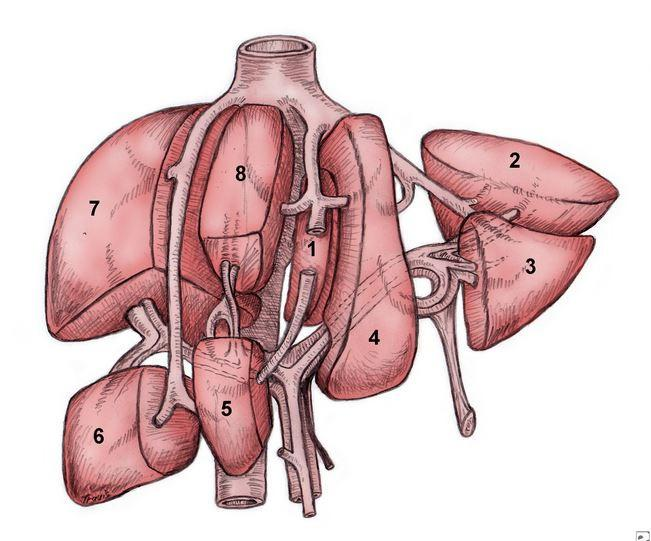
\includegraphics[width=0.5\textwidth]{Illustrations/segment.jpg}
\label{fig:segment} % Назва малюнку
\caption{Сегментарна будова печінки}
\end{figure}

Для оцінки стадії поширення пухлини печінки ключовим є розуміння судинної анатомії печінки, її сегментарної будови  (Рис. \ref{fig:segment}). 
Анатомія ворітної вени (MPV) майже завжди представляє собою головний стовбур, який у воротах печінки поділяється на дві великі гілки: ліву ворітну вену та праву ворітну вену. Однак, буває інша, варіантна атаномія ворітної вени, яка найчастіше представлена трифуркацією воріної вени, або інші варіанти.
Анатомія печінкових вен набагато більш варіабельна \cite{pmid22813792}. Поряд із класичною анатомією, при якій три великі вени печінки: ліва (LHV), серединна (MHV) і права (RHV) печінкові вени впадають в нижню порожнисту вену (IVC), безпосередньо перед впадінням в останню ліва печінкова вена (LHV) та серединна печінкова (MHV) зливаються у спільне устя, існують інші варіанти \cite{pmid22835780}. 
Для орієнтиру середнинної печінкової вени використовують ложе жовчного міхура. Додаткові праві задні нижні печінкові вени не використовують у якості орієнтирів для стадіювання по PRETEXT (Таб. \ref{table:PRETEXTTable}).

\begin{table}[]
\caption{Cтадіювання гепатобластом по PRETEXT.}
\resizebox{\textwidth}{!}{%
\begin{tabular}{|p{0.2\linewidth}|p{0.7\linewidth}|}
\hline
\textbf{PRETEXT} & \multicolumn{1}{c|}{\textbf{Визначення}}                              \\ \hline
\textit{I}       & пухлина в межах 1 секції печінки, 3 суміжні секції вільні від пухлини \\ \hline
\textit{II}      & 1 або 2 секції залучені, 2 суміжні секції вільні від пухлини          \\ \hline
\textit{III}     & 2 або 3 секції залучені, 1 суміжна секція вільна від пухлини          \\ \hline
\textit{IV}      & 4 секції печінки охоплені пухлиною, немає вільної суміжної секції     \\ \hline
\end{tabular}%
}
\label{table:PRETEXTTable}
\end{table}

\begin{figure}[h]
\centering
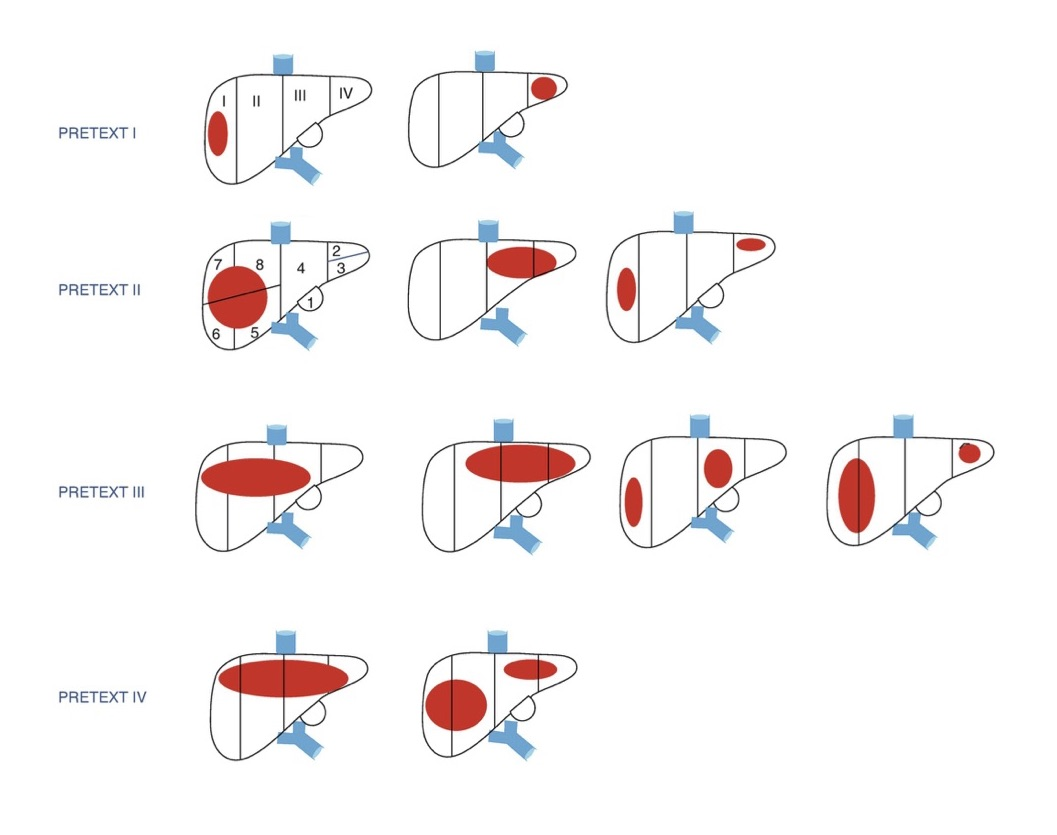
\includegraphics[width=0.9\textwidth]{Illustrations/pretexmal.jpg}
\label{fig:pretexmal} % Назва малюнку
\caption{Cтадіювання гепатобластом по PRETEXT}
\end{figure}

\subsubsection{PRETEXT I}
При цій стадії пухлина знаходиться виключно в правій задній секції печінки (сегменти 6 та/або 7)  або в лівій латеральній секції печінки (сегменти 2 та/або 3) і майже завжди резектабельна. Дуже малі пухлини найчастіше діагностуються при скринінгу або як акцидентальна знахідка. Але частіше виявляються пухлини більших розмірів. 
\subsubsection{PRETEXT II}
PRETEXT II  пухлини майже завжди є однофокальними і обмежені правою або лівою долями печінки. Спочатку не було окремо класифіковано пухлини, що розміщуються лише в хвостатій долі (сегмент 1). Наразі пухлини локалізовані в сегменті 1 додатково класифікуються як С1.
\subsubsection{PRETEXT III}
Найважливішим завданням цієї класифікації є відрізнити PRETEXT III від PRETEXT IV. Це зробити легше для пухлин, які розташовані справа і відокремлені від лівої латеральної секції умбілікальною фісурою та ворітною веною. Коли пухлина локалізована ліворуч, основним анатомічним орієнтиром є права печінкова вена, яку часто важче ідентифікувати і яку слід відрізняти від допоміжних вен, що впадають у нижню порожнисту вену (IVC).
\subsubsection{PRETEXT IV}
При даному ураженні пухлини охоплюють усі чотири відділи печінки, і тому, за надзвичайно рідкісними вийнятками, неможливо виконати видалення пухлини без трансплантації печінки. Результати досліджень SIOPEL свідчать про те, що багато дітей з великою однофокальною гепатобластомою PRETEXT IV перенесли трисекціонектомію після передопераційної хіміотерапії. Також є дані про мультифокальні гепатобластоми з PRETEXT IV, які також успішно лікуються без трансплантації. Незважаючи на ці спостереження, усіх пацієнтів з PRETEXT IV слід направляти на оцінку до центру трансплантації.

% Please add the following required packages to your document preamble:
% \usepackage{graphicx}
% \usepackage[table,xcdraw]{xcolor}
% If you use beamer only pass "xcolor=table" option, i.e. \documentclass[xcolor=table]{beamer}
\begin{table}[]
\caption{Субкласифікація PRETEXT}
\label{table:subPRETEXT}
\centering
\resizebox{\textwidth}{!}{%
\begin{tabular}{|
>{\columncolor[HTML]{FFFFFF}}c |
>{\columncolor[HTML]{FFFFFF}}l |}
\hline
\textbf{Субкласифікація} & \textbf{Визначення}                                                   \\ \hline
\textit{M}               & Віддалені метастази (легені)                                    \\ \hline
\textit{P}               & Інвазія пухлини в праву і ліву гілки портальної вени або в біфуркацію \\ \hline
\textit{V}               & Інвазія пухлини у нижню порожнисту вену або в печінкові вени          \\ \hline
\textit{F}               & Мультифокальна пухлина                                                \\ \hline
C                        & Пухлина каудальної долі                                               \\ \hline
E                        & Суміжна позапечінкова пухлина                                         \\ \hline
R                        & Спонтанний розрив пухлини                                             \\ \hline
\end{tabular}%
}
\end{table}



\subsubsection{Мультифокальна пухлина (F)}
При діагностиці гепатобластом важливою є також диференціація між уніфокальним та мультифокальним ростом пухлин \cite{pmid24132546}. Наявність більш ніж одного внутрішньопечінкового вузлика, незалежно від розміру або групи PRETEXT, класифікується як F1, а одиничне ураження як F0 \ref{table:subPRETEXT}.
\subsubsection{Судинні інвазії (P, V)}
При гепатобластомі так як і при гепатоцелюлярній карциномі досить часто спостерігається інвазія пухлин як в ворітну вену так і в печінкові вени та/або нижню порожнисту вену. Згідно PRETEXT 2005 року поняття інвазія досить чітко окреслено: перший тип - це інвазія в просвіт вени і другий - це повне проростання вени, з обструкцією її просвіту або без нього. Припускається, що вена інвазована, якщо в проекції її розташування не візуалізується жодна судина у відповідній фазі контрастуванян. Хоча обидва варіанти є поганими прогностичними факторами. 
Інвазія або лівої ворітної вени LPV, або правої ворітної вени RPV, або однієї з їх основних гілок класифікується як P1. При інвазії обох гілок ворітної вени та/або MPV пацієнт класифікується як Р2.
Залучення однієї або двох печінкових вен або їх основних притоків класифікується як V1 або V2, відповідно. Термін V3 використовується, коли є ураження всіх трьох печінкових вен та/або IVC. Компресія IVC дуже часто спостерігається у дітей з великими пухлинами, часто супроводжується збільшенням напівнепарної вени.
У кожному випадку втягнення вен (на відміну від огортання) позначається суфіксом –a.
\subsubsection{Позапечінкове поширення пухлини (E, H)}
Система PRETEXT класифікує пряме поширення пухлини з печінки та перитонеальне поширення пухлини як E1, E1a, E2 або E2a \cite{pmid23217875}. Крім того, при обстеженні також встановлюється наявність (H1) або відсутність (H0) розриву пухлини. Хоча немає жодних доказів того, що E1, E2 або H1 є несприятливим прогнозом.

Первинна пухлина печінки може проростати в черевну стінку, діафрагму або сусідні органи, такі як підшлункова залоза або товста кишка \cite{pmid23331862}. Пряме проростання пухлини класифікується як Е1. Проростання лише в жовчний міхура не слід розглядати як E1.
Канцероматоз очеревини у вигляді окремих пухлинних вузликів часто можна виявити за допомогою КТ або МРТ особливо у пацієнтів з асцитом (рис. 8.13; \cite{pmid23831416}. Це поширення класифікується як E2, незалежно від розміру ураження.

Невідомо, чи наявність асциту є незалежним фактором ризику у дітей з первинними пухлинами печінки. Для полегшення подальшого аналізу даних до класифікації додається суфікс –a (тобто E0a, E1a або E2a), коли присутній асцит.

Розрив пухлини класифікується як Н1. Зазвичай це проявляється  клінічниими, лабораторними та візуалізаційними методами досліджень. Наприклад, поява раптового болю у животі, можливо, після травми, гіпотонія або зниження рівня гематокриту та поява ехогенної рідини в черевній порожнині на УЗД, або аспірація крові при пункції. Розрив пухлини не рідкість для пацієнтів з гепатобластомою \cite{pmid24132546}, і може знадобитися термінова операція або емболізація. Локалізовані (наприклад, субкапсульні) крововиливи та кровотечі, пов’язані з біопсією, не класифікуються як H1.
\subsubsection{Метастатична хвороба (M, N)}
Як і у дорослих, гематогенні метастази пухлини класифікуються як M1. При гепатобластомі майже всі метастази при діагностиці виявляються в легенях (M1p), але при інших пухлинах, наприклад гепатоцелюлярній карциномі іноді зустрічаються в скелеті (M1s), центральній нервовій системі (M1c), кістковому мозку (M1m) або інших ділянках (M1x). Підтверджувати метастаз біопсією при наявності переконливих даних не потрібно.  

Хоча мультидетекторна технологія КТ зараз широко доступна, якісна візуалізація всієї поверхні легенів часом неможлива з різних причин, незважаючи на анестезію або седацію пацієнтів. Навіть при ідеальній візуалізації діагностика легеневих метастазів у дітей складна \cite{pmid24362406}. Різні доброякісні ураження можуть імітувати поодинокі або множинні метастази. Найпоширеніші з них - гранульоми, які можна спостерігати після бактеріальних, грибкових або вірусних інфекцій (наприклад, туберкульозу, гістоплазмозу та вітряної віспи). Гамартоми та внутрішньолегеневі лімфатичні вузли також можуть імітувати метастази.

Система PRETEXT застосовує прагматичний підхід до вирішення цієї проблеми. Замість того, щоб наполягати на біопсії у всіх пацієнтів із ураженнями легень, сумісними з метастазами, він класифікує їх як M1p і залишає рішення про стратифікацію ризику (наприклад, на основі розміру та/або кількості уражень) для індивідуального лікування. 

Метастази в лімфатичні вузли є рідкісними при гепатобластомі \cite{pmid24734315}, і навіть коли вони є, на даний момент не до кінця зрозуміло чи вони є значущим прогностичним фактором \cite{pmid24757164}. Також вони можуть бути збільшені внаслідок запального процесу. З цих причин по системі PRETEXT необхідно підтвердження біопсії. У перспективі виявлення злоякісних вузлів за допомогою позитронно-емісійної томографії або дифузійно-зваженого МРТ. В даний час найкращим підходом може бути біопсія дуже великих вузлів (> 15 мм у ширину) у дітей з гепатобластомою \cite{pmid24759227}. 

Метастази в черевні лімфатичні вузли кодуються як N1, а віддалені вузлові метастази як N2.
\subsection{Післяопераційна класифікація Children’s Oncology Group }

Згідно цієї класифікації при I стадії у пацієнта відсутні метастази і пухлина повністю резектована. При ІІ стадії відсутні метастази, немає мікроскопічної інвазії після резекції пухлини або розриву пухлини (включаючи розрив пухлини під час операції). При ІІІ стадії немає віддалених метастазів, пухлини нерезектабельні або резектовані з грубими залишковими вогнищами або є метастази у лімфатичні вузли. При ІV стадії є віддалені метастази, не залежно від місцевого поширення пухлини \cite{pmid24852330}.

% Please add the following required packages to your document preamble:
% \usepackage{graphicx}
% \usepackage[table,xcdraw]{xcolor}
% If you use beamer only pass "xcolor=table" option, i.e. \documentclass[xcolor=table]{beamer}

\begin{table}[]
\small
\caption{Післяопераційна класифікація Children’s Oncology Group\cite{pmid24852330}}
\label{table:subPRETEXT}

\centering

\normalsize
\begin{tabular}{|p{0.15\linewidth} | p{0.6\linewidth}|}
\hline
\textbf{Стадія}                                    & \textbf{Визначення}                                                                     \\ \hline
{\color[HTML]{202124} \textit{\textbf{Стадія I}}}  & {\color[HTML]{202124} Відсутні метастатичні захворювання, пухлина повністю резектована} \\ \hline
{\color[HTML]{202124} \textit{\textbf{Стадія IІ}}} &
  {\color[HTML]{202124} Відсутність метастатичного захворювання, 
  мікроскопічного залишкового захворювання після резекції пухлини або розриву пухлини 
  (включаючи розрив пухлини під час операції)} \\ \hline
{\color[HTML]{202124} \textit{\textbf{Стадія IІI}}} &
  {\color[HTML]{202124} Немає віддалених метастазів, 
  пухлини нерезектабельні або 
  резектовані з грубими залишковими вогнищами
  або є метастази у лімфатичні вузли} \\ \hline
{\color[HTML]{202124} \textit{\textbf{Стадія IV}}} & {\color[HTML]{202124} Віддалені метастази, незалежно від місцевого поширення пухлини}      \\ \hline
\end{tabular}%

\end{table}


% Please add the following required packages to your document preamble:
% \usepackage{graphicx}
% \usepackage[table,xcdraw]{xcolor}
% If you use beamer only pass "xcolor=table" option, i.e. \documentclass[xcolor=table]{beamer}
\begin{table}[]
\centering
\caption{Групи ризику гепатобластом по системі CHICS (Children’s Hepatic Tumors International Collaboration`s Stratification)}
\label{tab:risk}
\resizebox{\textwidth}{!}{%
\begin{tabular}{{|p{0.15\linewidth} | 
                  p{0.15\linewidth}|
                  p{0.15\linewidth}|
                  p{0.15\linewidth}|
                  p{0.15\linewidth}|
                  }}
\hline
\textbf{Групи ризику} &
  {\color[HTML]{231F20} \textbf{LR (low risk) – група низького ризику}} &
  {\color[HTML]{231F20} \textbf{IR (intermediate risk) – група среднього ризику}} &
  {\color[HTML]{231F20} \textbf{HR (high risk) – група високого ризику}} &
  {\color[HTML]{231F20} \textbf{VHR (very high risk) – група вкрай високого ризику}} \\ \hline
{\color[HTML]{231F20} \textit{\textbf{Метастази}}} &
  {\color[HTML]{231F20} \textbf{М(-)}} &
  {\color[HTML]{231F20} \textbf{М(-)}} &
  {\color[HTML]{231F20} \textbf{М(-)}} &
  {\color[HTML]{231F20} \textbf{М(+)}} \\ \hline
{\color[HTML]{231F20} \textit{\textbf{I}}} &
  {\color[HTML]{231F20} VPERF—, (будь-який AFP, будь-який вік)} &
  {\color[HTML]{231F20} -} &
  {\color[HTML]{231F20} VPERF+ , та вік \textless{}8 років (будь-який AFP)} &
  {\color[HTML]{231F20} VPERF+, і вік ≥8 років} \\ \hline
{\color[HTML]{231F20} \textit{\textbf{II}}} &
  {\color[HTML]{231F20} VPERF—, вік \textless 3 років та AFP \textgreater{}1,000 ng/mL} &
  {\color[HTML]{231F20} VPERF—, вік \textless 3 років, та AFP 100-1,000 ng/mL} &
  {\color[HTML]{231F20} Вік 3-7 роки, та/або VPERF +} &
  {\color[HTML]{231F20} AFP \textless{}100 ng/mL, та/або вік ≥8 років} \\ \hline
{\color[HTML]{231F20} \textit{\textbf{III}}} &
  {\color[HTML]{231F20} -} &
  {\color[HTML]{231F20} VPERF—, та вік \textless 3 років, та AFP \textgreater{}1,000 ng/mL} &
  {\color[HTML]{231F20} Вік 3-7 роки, та/або VPERF+, та/або AFP 100-1,000 ng/mL} &
  {\color[HTML]{231F20} AFP \textless{}100 ng/mL, та/або вік ≥8 років} \\ \hline
{\color[HTML]{231F20} \textbf{IV}} &
  {\color[HTML]{231F20} -} &
  {\color[HTML]{231F20} -} &
  {\color[HTML]{231F20} AFP \textgreater{}100 ng/mL} &
  {\color[HTML]{231F20} AFP \textless{}100 ng/mL, та/або вік ≥8 років} \\ \hline
\end{tabular}%
}
\end{table}


\begin{figure}[h]
\centering
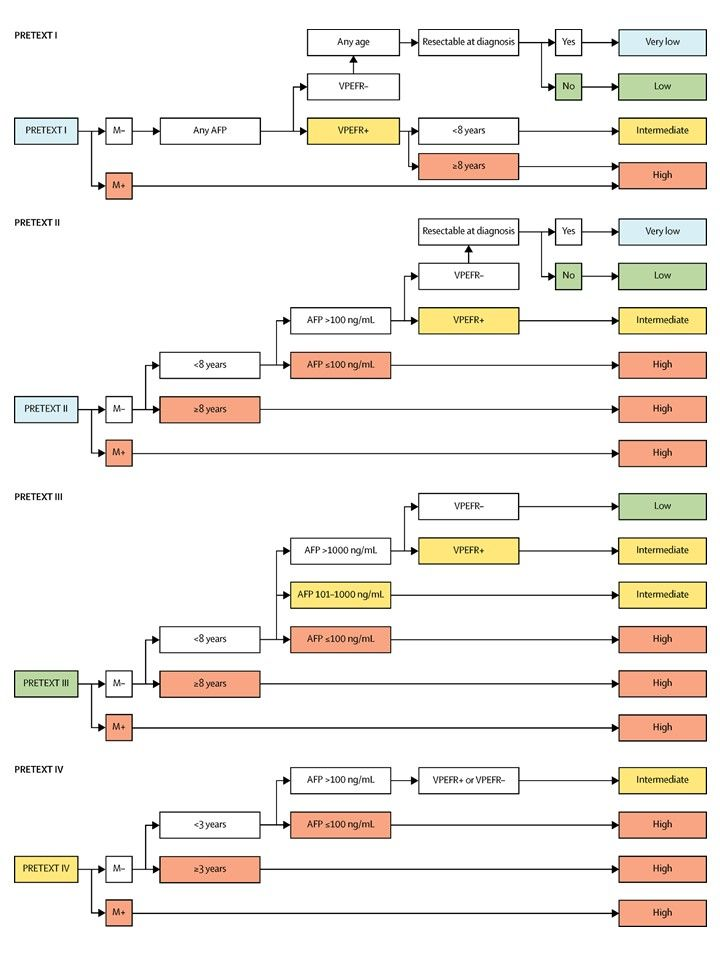
\includegraphics[width=0.9\textwidth]{Illustrations/risk.jpg}
\label{fig:risk} % Назва малюнку
\caption{Групи ризику гепатобластом по системі CHICS (Children’s Hepatic Tumors International Collaboration`s Stratification)\cite{pmid24757164}}
\end{figure}
\chapter{МАТЕРІАЛИ ТА МЕТОДИ ДОСЛІДЖЕННЯ}
\section{Клінічна характеристика пацієнтів із гепатобластомою}
Для вирішення поставлених задач нами проведено комплексне дослідження пацієнтів з гепатобластомою печінки, яких було прооперовано у відділенні трансплантації і хірургії печінки Національного інституту хірургії та трансплантології імені О.О. Шалімова за період із січня 2005 по січень 2020 р. Всього було прооперовано 90 дітей з гепатобластомою, з яких 81 пацієнту виконана резекція печінки, а в 9 випадках нерезектабельної гепатобластоми виконана трансплантація частини печінки від живого родинного донора (Рис. \ref{fig:90-81-9}). 

\begin{figure}[h]
\centering
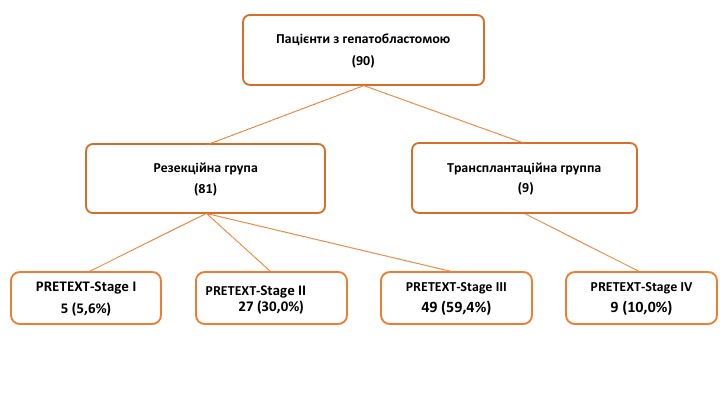
\includegraphics[width=0.9\textwidth]{Illustrations/90-81-9.jpeg}
\label{fig:90-81-9} % Назва малюнку
\caption{Структура дослідження.}
\end{figure}


Розподілення пацієнтів за віком та статтю наведено у діаграмі (Рис. \ref{fig:mw})


\begin{figure}[h]
\centering
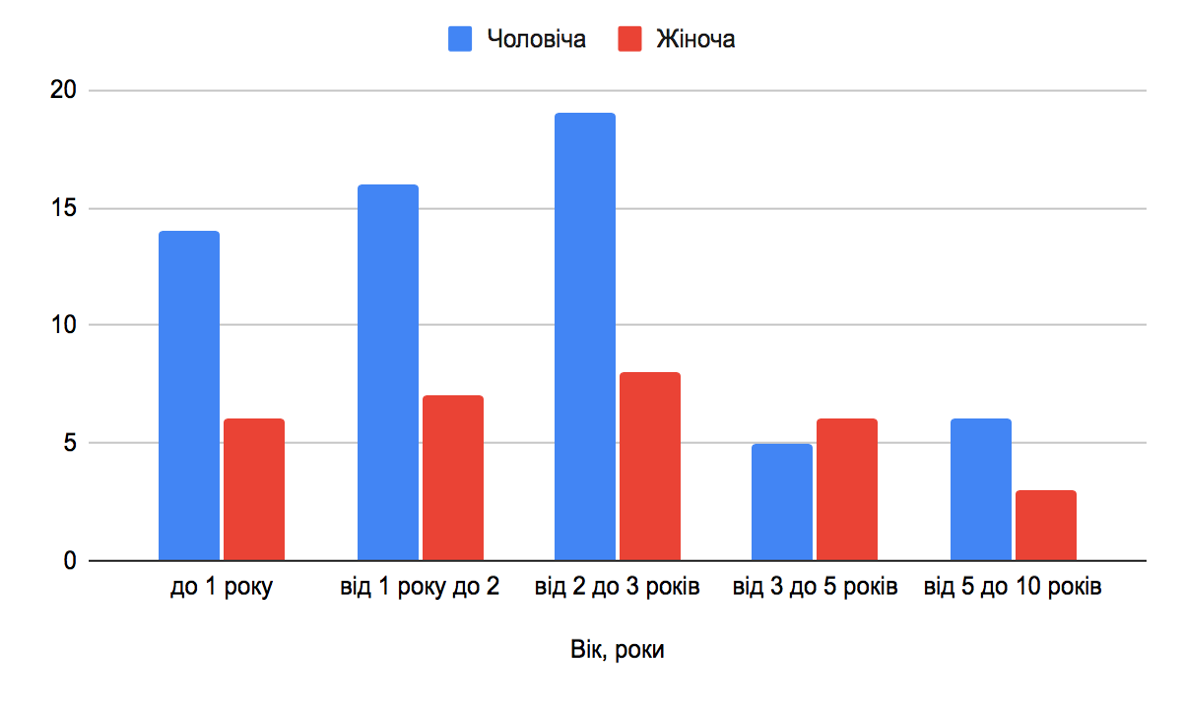
\includegraphics[width=0.7\textwidth]{Illustrations/mw.png}
\label{fig:mw} % Назва малюнку
\caption{Розподілення пацієнтів за віком та статтю.}
\end{figure}


\begin{table}[]
\centering
\caption{Розподілення пацієнтів по статі.}
\label{tab:sex}
\begin{tabular}{|p{0.1\linewidth}|p{0.1\linewidth}|p{0.1\linewidth}|}
\hline
\textbf{Стать}    & {\color[HTML]{231F20} \textbf{Кількість}} & {\color[HTML]{231F20} \textbf{\%}} \\ \hline
\textbf{Чоловіча} & 59                                        & 65,5\%                            \\ \hline
\textbf{Жіноча}   & 31                                        & 34,4\%                            \\ \hline
\end{tabular}
\end{table}

Із 90 пацієнтів 59 було чоловічої статі та 31 жіночої (Таб. \ref{tab:sex}). 66 пацієнтів було віком до 3 років, що склало 76,7\%. Дітей віком до 1 року було всього 20, що склало 23,3\%; віком від 1 до 2 років 22, що склало 25,8\%; від 2 до 3 років – 24 пацієнта (27,9\%); 20 пацієнтів з 3 до 10 років, що склало 23,3\%.

В нашій работі ми використовували Брисбанську класификацію анатомії сегментів печінки та відповідних резекцій печінки комітету Гепато-панкреато-біліарної Асоціації (2000 р.) \cite{pmid24852330}, яка базується на сегментарній будові печінки по C.Cuonoud. Класифікація базується на поділі печінки на секції, сектори та сегменти відповідно поділу портальних структур першого, другого та третього порядку. Згідно класифікації виділяють: 

\begin{itemize}
    \item Поділ першого порядку
    \begin{itemize}
    \item Ліва напівпечінка (Sg 2-4 ± Sg1 по C.Cuonoud), операція - лівобічна гемігепатектомія
    \item Права напівпечінка (Sg 5-8 ± Sg1 по C.Cuonoud), операція - правобічна гемігепатектмія
\end{itemize}
\end{itemize}
\begin{itemize}
    \item Поділ другого порядку
    \begin{itemize}
    \item Ліва латеральна секція (Sg 2-3 ± Sg1 по C.Cuonoud), операція - лівобічна латеральна секціоектомія
    \item Ліва медіальна секція (Sg 4 по C.Cuonoud), операція - лівобічна медіальна секціоектомія
    \item Права передня секція (Sg 5-8 по C.Cuonoud), операція - правобічна передня секціоектомія
    \item Права задня секція (Sg 6-7 по C.Cuonoud), операція - правобічна задня секціоектомія
\end{itemize}
\end{itemize}
    \begin{itemize}
    \item Поділ третього порядку
    \begin{itemize}
    \item Сегменти з 1-го по 9-й, операція - сегментектомія відповідних сегментів
    \item Два суміжних сегменти ((Sg 5-6, Sg 7-8, Sg 1-9), операція - бісегментектомія
\end{itemize}
\end{itemize}

Для резекцій 3 секцій печінки використовують назви лівобічна (Sg 2-5, Sg 8 ± Sg1 по C.Cuonoud) та правобічна  (Sg 4-8 ± Sg1 по C.Cuonoud) трисекціоектомії.

Пацієнти були оцінені за шкалою дохірургічної оцінки  гепатобластом у дітей PRETEXT (pre-treatment extent of disease) відповідно рекомендацій SIOPEL (Рис. \ref{fig:pretexpac}). За цією шкалою стадія PRETEXT визначається на підставі поширення пухлини на секції печінки за даними МРТ або КТ і включають наступні критерії: 
PRETEXT I – пухлина виявлена в межах однієї секції печінки; 
PRETEXT II – у двох секціях печінки; 
PRETEXT III – пухлина виявлена у трьох секціях печінки, вільна від пухлини тільки одна секція; 
PRETEXT IV – рак виявлений у всіх чотирьох секціях печінки. 

\begin{figure}[h]
\centering
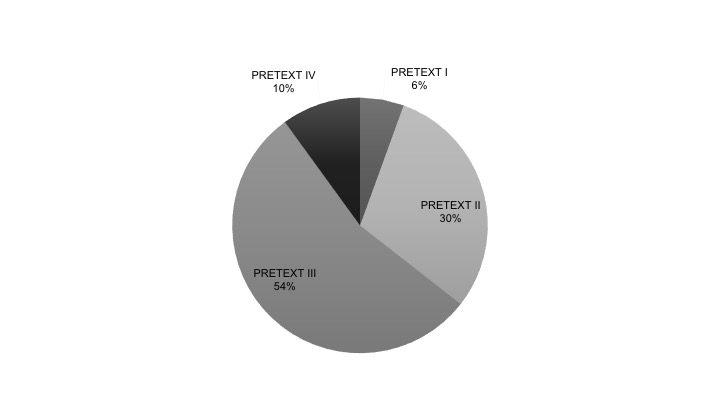
\includegraphics[width=0.9\textwidth]{Illustrations/pretexpac.jpeg}
\label{fig:pretexpac} % Назва малюнку
\caption{Розподіл пацієнтів за класифікацією PRETEXT.}
\end{figure}


Резекція печінки була виконана при гепатобластомі PRETEXT-I, II, III, як первинна резекція у 79 дітей, і в 2-х випадках при рецидивній гепатобластомі виконана ререзекція печінки. При нерезектабельній гепатобластомі PRETEXT-IV з пухлинним ураженням всіх секцій печінки і PRETEXT-III з настільки близьким розташуванням до судин воріт печінки або печінкових вен, що малоймовірно досягнути «tumor free margin» резекційної площини, при відсутності за даними КТ і МРТ віддалених метастазів, виконана трансплантація печінки у 9 випадках.

Згідно класифікації PRETEXT І стадію було встанолено у 5 пацієнтів, що відповідає 5,6\%, ІІ стадія у 27 пацієнтів – 30,0\%, ІІІ стадія у 49 пацієнтів – 54,4\%, та ІV стадія у 9 пацієнтів – 10,0\% (Рис. \ref{fig:pretexpac}).

Більш детальна характеристика пацієнтів згідно класифікації PRETEXT та її субкласифікації наведено у таблиці (Таб. \ref{tab:pretexpvfc})

% Please add the following required packages to your document preamble:
% \usepackage{graphicx}
% \usepackage[table,xcdraw]{xcolor}
% If you use beamer only pass "xcolor=table" option, i.e. \documentclass[xcolor=table]{beamer}
\begin{table}[]
\centering
\caption{Розподілення пацієнтів по стадії PRETEXT }
\label{tab:pretexpvfc}
\resizebox{\textwidth}{!}{%
\begin{tabular}{|p{0.2\linewidth}|
                 p{0.2\linewidth}|
                 p{0.2\linewidth}|
                 p{0.2\linewidth}|}
\hline
\textbf{} &
  {\color[HTML]{231F20} \textbf{Резекційна група (n=81)}} &
  {\color[HTML]{231F20} \textbf{Трансплантаційна група (n=9)}} &
  {\color[HTML]{231F20} \textbf{Значимість відмінностей, p}} \\ \hline
\textbf{PRETEXT I}                           & 5  & - & \textbf{0,03} \\ \hline
\textbf{PRETEXT IІ}                          & 27 & - & \textbf{0,04} \\ \hline
\textbf{PRETEXT IІІ}                         & 49 & - & \textbf{0,02} \\ \hline
\textbf{PRETEXT IV}                          & -  & 9 & \textbf{0,02} \\ \hline
\textbf{P (Інвазія в ворітну вену)}          & 3  & 5 & \textbf{0,03} \\ \hline
\textbf{V (Інвазія в печінкові вени, НПВ)}   & 9  & 6 & \textbf{0,04} \\ \hline
\textbf{F (Мультифокальна пухлина)}          & 56 & 9 & \textbf{0,02} \\ \hline
\textbf{С (Поширення на SgI)}                & 49 & 8 & \textbf{0,02} \\ \hline
\textbf{E (Позапечінкове поширення пухлини)} & 3  & 1 & \textbf{0,03} \\ \hline
\textbf{R (Спонтанний розрив пухлини)}       & 2  & 0 & \textbf{0,04} \\ \hline
\textbf{M (Віддалені метастази)}             & 0  & 0 & \textbf{0,02} \\ \hline
\textbf{Інвазія в жовчні протоки}            & 1  & 5 & \textbf{0,02} \\ \hline
\end{tabular}%
}
\end{table}

В стандартний доопераційний протокол обстеження крім СКТ та МРТ також обов’язково входили загальний та біохімічний аналіз крові, коагулограма, визначення рівня альфа-фетопротеїну (АФП). У таблиці наведено основні показники, які характеризують пацієнтів  з гепатобластомами у двох групах: резекційній та трансплантаційній групах. Статистично значущих відмінностей між групами не виявлено, крім одного критерію – рефрактерність до хіміотерапії була значно вищою у трансплантаційній групі (Таб. \ref{tab:haracter}). Це пов’язано, передусім, з тим, що у трансплантаційній групі у 78\% випадків при патогістологічному аналізі спостерігався змішаний епітеліально-мезенхімальний тип гепатобластоми, як правило, нечутливий до хіміотерапії. 


\begin{table}[]
\centering
\caption{Основні характеристики резекційної та трансплантаційної груп пацієнтів із гепатобластомою}
\label{tab:haracter}
\resizebox{\textwidth}{!}{%
\begin{tabular}{|p{0.2\linewidth}|
                 p{0.2\linewidth}|
                 p{0.2\linewidth}|
                 p{0.2\linewidth}|}
\hline
\textbf{Xapaктepнcтнкa} &
  {\color[HTML]{231F20} \textbf{Peзeкційнa rpyпa (n=81)}} &
  {\color[HTML]{231F20} \textbf{Tpaнcплaнтaційнa rpyпa (n=9)}} &
  {\color[HTML]{231F20} \textbf{P}} \\ \hline
{\color[HTML]{231F20} \textit{\textbf{Biк, мic.}}} &
  {\color[HTML]{231F20} \textbf{28 (6-59)}} &
  {\color[HTML]{231F20} \textbf{39 (8-66)}} &
  {\color[HTML]{231F20} \textbf{0,65}} \\ \hline
{\color[HTML]{231F20} \textit{\textbf{Cтaть (ч/ж)}}} &
  {\color[HTML]{231F20} 58/23} &
  {\color[HTML]{231F20} 6.3} &
  {\color[HTML]{231F20} 0,84} \\ \hline
{\color[HTML]{231F20} \textit{\textbf{Heoaд’ювaнтнa xiмioтepaпiя, n (\%)}}} &
  {\color[HTML]{231F20} 65 (80\%)} &
  {\color[HTML]{231F20} 9 (100\%)} &
  {\color[HTML]{231F20} 0,2} \\ \hline
{\color[HTML]{231F20} \textit{\textbf{AFP більше 100 ng/ml, n (\%)}}} &
  {\color[HTML]{231F20} 60 (74\%)} &
  {\color[HTML]{231F20} 9 (100\%)} &
  {\color[HTML]{231F20} 0,18} \\ \hline
\textbf{Позaпeчiнкoвi мeтacтaзи, n(\%)}         & 4 (7\%)     & −          & 0,48   \\ \hline
\textbf{Бiлipyбiн (mmol/l)}                     & 24,7±7,2    & 28,3±9,5   & 0,56   \\ \hline
\textbf{ACT (U/L)}                              & 52,7±7,4    & 65,2±8,6   & 0,74   \\ \hline
\textbf{AЛT (U/L)}                              & 67,6±6,3    & 76,4±7,3   & 0,76   \\ \hline
\textbf{Пpoтpoмбінoвий чac, c}                  & 17,6±1,2    & 18,5±2,5   & 0,85   \\ \hline
\textbf{Peфpaктepнicть дo xiмioтepaпiï, n (\%)} & 20 (24,7\%) & 5 (66,6\%) & 0,034* \\ \hline
\end{tabular}%
}
\end{table}

Основна частина пацієнтів була з верифікованими патогістологічними діагнозами після обов'язкової біопсії пухлини, за винятком 12 випадків (14,8\%) гепатобластоми PRETEXT I-II, коли виконана первинна резекція печінки без неоад’ювантної ХТ. Патогістологічна характеристика пацієнтів наведена у талиці (Таб. \ref{tab:patolpac})


\begin{table}[]
\centering
\caption{Розподіл пацієнтів згідно патогістологічних типів та підтипів гепатобластом.}
\label{tab:patolpac}
\begin{tabular}{|p{0.2\linewidth}|
                 p{0.2\linewidth}|
                 p{0.2\linewidth}|
                 p{0.2\linewidth}|}
\hline
{\color[HTML]{231F20} \textbf{Тип}} &
  {\color[HTML]{231F20} \textbf{Підтип}} &
  {\color[HTML]{231F20} \textbf{Кількість пацієнтів}} &
  {\color[HTML]{231F20} \textbf{\%}} \\ \hline
\cellcolor[HTML]{FFFFFF}{\color[HTML]{231F20} } &
  {\color[HTML]{231F20} Фетальний підтип} &
  {\color[HTML]{231F20} 27} &
  {\color[HTML]{231F20} 30,0\%} \\ \cline{2-4} 
\cellcolor[HTML]{FFFFFF}{\color[HTML]{231F20} } &
  {\color[HTML]{231F20} Змішаний ембріональний / фетальний підтип} &
  {\color[HTML]{231F20} 16} &
  {\color[HTML]{231F20} 17,8\%} \\ \cline{2-4} 
\cellcolor[HTML]{FFFFFF}{\color[HTML]{231F20} } &
  {\color[HTML]{231F20} Макротрабекулярний підтип} &
  {\color[HTML]{231F20} 4} &
  {\color[HTML]{231F20} 4,4\%} \\ \cline{2-4} 
\multirow{-4}{*}{\cellcolor[HTML]{FFFFFF}{\color[HTML]{231F20} \textbf{Епітеліальний тип}}} &
  {\color[HTML]{231F20} Дрібноклітинний недиференційований підтип} &
  {\color[HTML]{231F20} 3} &
  {\color[HTML]{231F20} 3,3\%} \\ \hline
\cellcolor[HTML]{FFFFFF}{\color[HTML]{231F20} } &
  {\color[HTML]{231F20} Без тератоїдних особливостей} &
  {\color[HTML]{231F20} 19} &
  {\color[HTML]{231F20} 21,1\%} \\ \cline{2-4} 
\multirow{-2}{*}{Змішаний тип (епітеліальний та мезенхімальний)} &
  {\color[HTML]{231F20} З тератоїдними  особливостями} &
  {\color[HTML]{231F20} 18} &
  {\color[HTML]{231F20} 20,0\%} \\ \hline
{\color[HTML]{231F20} \textbf{Гепатобластома без додаткових особливостей (NOS)}} &
  {\color[HTML]{231F20} } &
  {\color[HTML]{231F20} 3} &
  {\color[HTML]{231F20} 3,3\%} \\ \hline
\end{tabular}
\end{table}

Для визначення алгоритму лікування гепатобластоми пацієнти були стратифіковані на групи ризику по системі Children’s Hepatic tumors International Collaboration—Hepatoblastoma Stratification (CHIC-HS) на основі найбільш прогностичних діагностичних факторів, які виявились при первинному аналізі: 

\begin{itemize}
    \item стадія PRETEXT; 
    \item вік молодший 3 років, 3–7 років та 8 років або старше;
    \item концентрація альфафетопротеїну (AFP) 100 нг/мл або нижче і 101-1000 нг/мл;
    \item наявність або відсутність метастазів;
    \item наявність або відсутність «VPEFR» : макроваскулярного ураження всіх печінкових вен (V) або портальної біфуркації (P), суміжної позапечінкової пухлини (E), мультифокальної пухлини (F) та спонтанного розриву пухлини (R).
\end{itemize}

При оцінці стану пацієнтів по системі CHICS було встановлено, що у 50 (55,6\%) пацієнтів був середній ризик за цією шкалою, у 24 (26,7\%) високий ризик, і у 16 (17,8\%) пацієнтів був дуже високий ризик  (Таб. \ref{tab:CHICS}). Питома вага пацієнтів з високим та дуже високим ступенем ризику був вищим у групі пацієнтів, яким виконали трансплантацію печінки в порівнянні з пацієнтами з резекціями печінки.




\begin{table}[]
\centering
\caption{Розподіл пацієнтів по групах ризику гепатобластом по системі CHICS (Children’s Hepatic Tumors International Collaboration`s Stratification)}
\label{tab:CHICS}
\resizebox{\textwidth}{!}{%
\begin{tabular}{|l|l|l|l|l|l|l|}
                 
\hline
\textbf{Групи ризику} &
  \multicolumn{2}{l|}{\cellcolor[HTML]{FFFFFF}{\color[HTML]{231F20} \textbf{Резекційна група}}} &
  \multicolumn{2}{l|}{\cellcolor[HTML]{FFFFFF}{\color[HTML]{231F20} \textbf{Транс\-план\-тац\-ійна група}}} &
  \multicolumn{2}{l|}{\cellcolor[HTML]{FFFFFF}\textbf{Разом}} \\ \hline
{\color[HTML]{231F20} \textit{\textbf{Середній ризик (IR)}}} &
  \multicolumn{1}{l|}{\cellcolor[HTML]{FFFFFF}{\color[HTML]{231F20} \textbf{50}}} &
  {\color[HTML]{231F20} \textbf{61,70\%}} &
  \multicolumn{1}{l|}{\cellcolor[HTML]{FFFFFF}{\color[HTML]{231F20} \textbf{-}}} &
  {\color[HTML]{231F20} \textbf{-}} &
  \multicolumn{1}{l|}{\cellcolor[HTML]{FFFFFF}50} &
  55,60\% \\ \hline
{\color[HTML]{231F20} \textit{\textbf{Високий ризик (HR)}}} &
  \multicolumn{1}{l|}{\cellcolor[HTML]{FFFFFF}{\color[HTML]{231F20} 20}} &
  {\color[HTML]{231F20} 24,70\%} &
  \multicolumn{1}{l|}{\cellcolor[HTML]{FFFFFF}{\color[HTML]{231F20} 4}} &
  {\color[HTML]{231F20} 44,40\%} &
  \multicolumn{1}{l|}{\cellcolor[HTML]{FFFFFF}24} &
  26,70\% \\ \hline
{\color[HTML]{231F20} \textit{\textbf{Дуже високий ризик (VHR)}}} &
  \multicolumn{1}{l|}{\cellcolor[HTML]{FFFFFF}{\color[HTML]{231F20} 11}} &
  {\color[HTML]{231F20} 13,60\%} &
  \multicolumn{1}{l|}{\cellcolor[HTML]{FFFFFF}{\color[HTML]{231F20} 5}} &
  {\color[HTML]{231F20} 55,60\%} &
  \multicolumn{1}{l|}{\cellcolor[HTML]{FFFFFF}16} &
  17,80\% \\ \hline
{\color[HTML]{231F20} \textit{\textbf{Разом}}} &
  \multicolumn{1}{l|}{\cellcolor[HTML]{FFFFFF}{\color[HTML]{231F20} 81}} &
  {\color[HTML]{231F20} } &
  \multicolumn{1}{l|}{\cellcolor[HTML]{FFFFFF}{\color[HTML]{231F20} 9}} &
  {\color[HTML]{231F20} } &
  \multicolumn{1}{l|}{\cellcolor[HTML]{FFFFFF}90} &
   \\ \hline
\end{tabular}%
}
\end{table}


\section{Клінічна характеристика донорів}
Згідно Закону України про трансплантацію органів та інших анатомічних матеріалів людини (№1007-XIV від 16.07.1999), та Закону України про застосування трансплантації анатомічних матеріалів від (№ 2427-VII  17.05.2018) ми обстежували близьких родичів реципієнтів, які виявили добровільне бажання стати донором частини печінки. Згода донорів та їх родинні зв'язки з реципієнтом підтверджено документально. 

Родинні зв'язки донора та реципієнта представлені в таблиці. Найчастіше, в 6 випадках (66,6\%), це була матір пацієнта, і в 3 (33,3\%) - батько пацієнта (Таб.\ref{tab:donorrec}). 

% Please add the following required packages to your document preamble:
% \usepackage[table,xcdraw]{xcolor}
% If you use beamer only pass "xcolor=table" option, i.e. \documentclass[xcolor=table]{beamer}
\begin{table}[]
\centering
\caption{Розподілення донорів по родинному зв'язку з реципієнтом.}
\label{tab:donorrec}
\begin{tabular}{|l|l|l|}
\hline
\textbf{Стать}  & {\color[HTML]{231F20} \textbf{Кількість}} & {\color[HTML]{231F20} \textbf{\%}} \\ \hline
\textbf{Матір}  & 6                                         & 66,7\%                             \\ \hline
\textbf{Батько} & 3                                         & 33,3\%                             \\ \hline
\end{tabular}
\end{table}

Всі донори були фізично та психологідно здоровими, не мали хронічної патології, інфекційних захворювань, що передаються трансмісивним шляхом. В 7 випадках реципієнт та донор мали однакову групу крові, у 2 - сумісну. Потенційним донорам, що несумісні по групах крові відмовляли в можливості доновання. Вікові обмеження для донорів складали 18-55 рокців. 
Шість пацієнтів (66,6\%) були жіночої статі, троє (33,3\%) - чоловічої (Таб.\ref{tab:donorsex}).


\begin{table}[]
\centering
\caption{Розподілення донорів по статі.}
\label{tab:donorsex}
\begin{tabular}{|p{0.2\linewidth}|
                 p{0.2\linewidth}|
                 p{0.2\linewidth}|}
\hline
\textbf{Стать}    &  \textbf{Кількість} & \textbf{\%} \\ \hline
\textbf{Жіноча}   & 6                                         & 66,7\%                             \\ \hline
\textbf{Чоловіча} & 3                                         & 33,3\%                             \\ \hline
\end{tabular}
\end{table}

Середній вік донорів склав 31,9±9,3 роки. 
Судинну анатомію вивчали за допомогою СКТ з внутрішньовенним контрастуванням до операції. Причому вивчали судинну анатомію ворітної та печінкової вени а також печінкової артерії. 
За допомогою СКТ проводили волюметрію майбутнього трансплантату. 

\section{Методи дослідження}
\subsection{Алгоритм доопераційного обстеження}

Всім пацієнтам з гепатобластомою проведено комплексне обстеження, що включає клінічні, інструментальні та спеціальні методи дослідження.
Діагностичний алгоритм включав наступні завдання:
\begin{enumerate}
    \item встановлення діагнозу гепатобластоми;
    \item диференціальна діагностика з доброякісними пухлинами;
    \item визначення рівня ураження жовчного дерева;
    \item вивчення судинної анатомії портальних і кавальних воріт печінки;
    \item виявлення інвазії пухлини в ворітну вену та печінкову артерію;
    \item виявлення віддалених метастазів;
    \item виявлення ураження регіональних лімфовузлів;
    \item визначення маси перспективного печінкового залишку;
    \item оцінка функціонального стану печінки;
\end{enumerate}

Обстеження починали зі збору клініко-анамнестичних даних. У пацієнтів з гепатобластомою брали до уваги скарги, наявність жовтяниці, температурну реакцію, перенесені оперативні втручання, супутню патологію, а також дані сімейного анамнезу. Наступним етапом проводили загальноклінічні дослідження, що включали загальний аналіз крові з лейкоцитарною формулою, загальний аналіз сечі, біохімічне дослідження крові, коагулограму. Також визначали онкомаркери Са 19-9, альфафетопротеїн, раково-ембріональний антиген. З метою виявлення супутнього вірусного гепатиту визначали маркери вірусних гепатитів В і С.

При оцінці показників загального аналізу крові, що включають гемоглобін, еритроцити, лейкоцити, тромбоцити, в досліджуваній групі і групі порівняння, не виявлено статистично значущої різниці (Таб. \ref{tab:ZAK})


\begin{table}[]
\centering
\caption{Показники загального аналізу крові.}
\label{tab:ZAK}
\begin{tabular}{|p{0.2\linewidth}|
                 p{0.2\linewidth}|
                 p{0.2\linewidth}|
                 p{0.2\linewidth}|}
\hline
{\color[HTML]{231F20} \textbf{Показник}} &
  {\color[HTML]{231F20} \textbf{Резекційна група (n=81)}} &
  {\color[HTML]{231F20} \textbf{Транс\-план\-таційна група (n=9)}} &
  {\color[HTML]{231F20} \textbf{Значимість відмінностей, p}} \\ \hline
{\color[HTML]{231F20} \textbf{Гемоглобін}} & {\color[HTML]{231F20} 125,6} & {\color[HTML]{231F20} 122,8} & 0,36 \\ \hline
{\color[HTML]{231F20} \textbf{Еритроцити}} & {\color[HTML]{231F20} 4,27}  & {\color[HTML]{231F20} 4,17}  & 0,67 \\ \hline
{\color[HTML]{231F20} \textbf{Лейкоцити}}  & {\color[HTML]{231F20} 8,6}   & {\color[HTML]{231F20} 7,45}  & 0,36 \\ \hline
{\color[HTML]{231F20} \textbf{Тромбоцити}} & {\color[HTML]{231F20} 311,5} & {\color[HTML]{231F20} 277,4} & 0,5  \\ \hline
\end{tabular}
\end{table}

 Показники біохімічного аналізу крові, що включають в себе показники загального та прямого білірубіну, загального білку, альбуміну, аланінамінотрансферази (АЛТ), аспартатамінотрансферази (АСТ), гамма-глютаматтрпнсфераза (ГГТП), лужної фосфатази (ЛФ) і лактатдегідрогенази (ЛДГ) були однорідними в обох групах (Таб. \ref{tab:BAK})

\begin{table}[]
\centering
\caption{Показники біохімічного аналізу крові.}
\label{tab:BAK}
\begin{tabular}{|p{0.2\linewidth}|
                 p{0.2\linewidth}|
                 p{0.2\linewidth}|
                 p{0.2\linewidth}|}
\hline
{\color[HTML]{231F20} \textbf{Показник}} &
  {\color[HTML]{231F20} \textbf{Резекційна група (n=81)}} &
  {\color[HTML]{231F20} \textbf{Транс\-план\-тацій\-на група (n=9)}} &
  {\color[HTML]{231F20} \textbf{Значимість відмінностей, p}} \\ \hline
{\color[HTML]{231F20} \textbf{Загальний білок}}     & {\color[HTML]{231F20} 72,8} & {\color[HTML]{231F20} 73,4} & 0,54 \\ \hline
{\color[HTML]{231F20} \textbf{Альбумін}}            & {\color[HTML]{231F20} 40,7} & {\color[HTML]{231F20} 41,4} & 0,91 \\ \hline
{\color[HTML]{231F20} \textbf{Білірубін загальний}} & {\color[HTML]{231F20} 24,7} & {\color[HTML]{231F20} 28,3} & 0,67 \\ \hline
{\color[HTML]{231F20} \textbf{Білірубін прямий}}    & {\color[HTML]{231F20} 19,9} & {\color[HTML]{231F20} 22,3} & 0,43 \\ \hline
\textbf{АЛТ}                                        & 67,6                        & 76,4                        & 0,18 \\ \hline
\textbf{АСТ}                                        & 52,7                        & 65,2                        & 0,42 \\ \hline
\textbf{ЛФ}                                         & 401,2                       & 316,11                      & 0,67 \\ \hline
\textbf{ЛДГ}                                        & 355,7                       & 389,4                       & 0,19 \\ \hline
\textbf{ГГТП}                                       & 351                         & 411,2                       & 0,58 \\ \hline
\end{tabular}
\end{table}


Оцінка показників коагулограми показала статистично значущу різницю міжнародного нормалізованого відношення (INR) і активованого часткового тромбопластинового часу (АЧТЧ) (p = 0,03 критерій Манна-Уїтні), а різниця показників протромбінового часу і індексу статистично незначущі (Таб. \ref{tab:KG})

\begin{table}[]
\centering
\caption{Показники коагулограми }
\label{tab:KG}
\begin{tabular}{|p{0.15\linewidth}|
                 p{0.15\linewidth}|
                 p{0.15\linewidth}|
                 p{0.15\linewidth}|}
\hline
{\color[HTML]{231F20} \textbf{Показник}} &
  {\color[HTML]{231F20} \textbf{Резекційна група (n=81)}} &
  {\color[HTML]{231F20} \textbf{Транс\-план\-тацій\-на група (n=9)}} &
  {\color[HTML]{231F20} \textbf{Значимість відмінностей, p}} \\ \hline
{\color[HTML]{231F20} \textbf{Про\-тромб\-іновий час}}    & {\color[HTML]{231F20} 17,6}  & {\color[HTML]{231F20} 18,5} & 0,08 \\ \hline
{\color[HTML]{231F20} \textbf{Про\-тромб\-іновий індекс}} & {\color[HTML]{231F20} 81,5}  & {\color[HTML]{231F20} 86,1} & 0,19 \\ \hline
{\color[HTML]{231F20} \textbf{INR}}                   & {\color[HTML]{231F20} 1,24}  & {\color[HTML]{231F20} 1,2}  & 0,09 \\ \hline
{\color[HTML]{231F20} \textbf{АЧТЧ}}                  & {\color[HTML]{231F20} 32,25} & {\color[HTML]{231F20} 30,2} & 0,12 \\ \hline
\end{tabular}
\end{table}




З інструментальних досліджень всім хворим в обов'язковому порядку виконували спіральну комп'ютерну томографію органів черевної порожнини і грудної клітки, магнітно-резонансна томографія, МРТ-холангіографію, УЗД черевної порожнини, УЗДС портальної системи і судин печінки, ЕКГ, ЕхоКГ, ФЕГДС і колоноскопію. 

Для вивчення судинної анатомії портальних і кавальних воріт печінки, виявлення інвазії пухлини в ворітну вену, печінкову артерію, наявності метастазування в регіональні лімфатичні вузли і віддалені органи виконували СКТ органів черевної порожнини і грудної клітки з внутрішньовенним підсиленням. Використовували спіральний комп'ютерний томограф LightSpeed-16 фірми General Electric c шириною зрізу 5 мм. Методику виконували наступним чином. Контрастування вісцеральних судин здійснювали за допомогою внутрішньовенного введення контрасту «Омніпак», в дозі 5 мл на 1 кг. ваги, але не більше 300 мл. Час за який контраст досягав печінкової артерії складав в середньому 18-27 секунд а печінкових вен - 50-80 секунд. Отримані зрізи обробляли і перетворювали в 3-х мірне зображення судинного русла. Для оцінки ступеня гепатоза печінки хворого, порівнювали денситометричну щільність печінки та селезінки.

За допомогою СКТ проводили волюметрію перспективного печінкового залишку і обсяг  частини печінки, що видаляється. Для виконання волюметрії печінки виконували роздруківку на плівці послідовних КТ-зрізів паренхиматозної фази виведення контрасту починаючи від рівня правого купола діафрагми і включаючи всі зрізи із зображенням печінки. Всі зрізи друкували з одним і тим же збільшенням, а на одному зі зрізів вказували лінійку масштабу, що відповідає 10 см.

\[ V = 100 * \frac{\sum_{} (S)}{l^2}*h \]
де 
V - об'єм вимірюваного сегмента печінки в см$^3$
Σ (S) - сума площ всіх зрізів вимірюваного сегмента печінки в пікселях
l - довжина масштабної 10-сантиметрової лінійки в пікселях
h - інтервал між зрізами томографа в сантиметрах

Магнітно-резонансну томографію та МРТ холангіографію виконували з метою візуалізації рівня ураження жовчного дерева, інвазії пухлини в вісцеральні судини і метастатичного ураження лімфатичних вузлів.  Дослідження виконували на магнітно-резонасному томографі Siemens Magnetom Avanto 1,5 тесла, c використанням внутрішньовенного контрасту «Магневіст». Метод МРТ дифузії печінки дозволяє диференціювати доброякісні та злоякісні стриктури жовчних протоків. Зображення, одержувані в ході МРТ холангіографії, дозволяють оцінити поширення пухлини вздовж жовчних протоків та визначити тип ураження згідно класифікації Bismuth-Corlette. Це ключове дослідження для визначення резектабельності та планування об'єму резекції печінки.

Ультразвукове дослідження органів черевної порожнини проводили всім пацієнтам за допомогою УЗ сканерів SSD 120 і SSD 256 фірми «Aloka» з конвексним датчиком частотою 3,5-5,0 МГц для дослідження стану печінки, виявлення розширення жовчних протоків, рівня блоку жовчних протоків, розмірів селезінки, виявлення асциту та інших рідинних скупчень, анатомічних взаємовідносин органів, виявлення супутньої патології.

УЗДС судин печінки проводили з метою первинного вивчення анатомії внутрішньопечінкових судин і судин портальної системи в передопераційному періоді та подальшого післяопераційного контролю кровотоку в печінковому залишку. Всіх хворих досліджували вранці, натщесерце. Дослідження проводилося на сканері «Tehnos» МРХ (ESACOTE SPA – Італія), з використанням конвексного датчика частотою 3,5-5,0 МГц. Застосовувалися режими сіро-шкального сканування, колірного і енергетичного допплерівського картування, імпульсно-хвильової доплерографії та їх різні комбінації. Дослідження починали в положенні хворого лежачи на спині через трансабдомінальний доступ з частотою датчика 5,0 МГц. Наступним етапом виконували черезреберне сканування в положенні хворого на спині, при необхідності використовували поворот хворого на лівий бік. Використовували сагітальне, горизонтальне і косе сканування з метою візуалізації стовбура ворітної вени та її гілок, власної печінкової артерії і її гілок, системи печінкових вен і НПВ. При неадекватній візуалізації частоту датчика зменшували до 3,5 МГц.

Кольорове допплерівське сканування здійснювали з використанням швидкісної шкали середньої швидкості кровотоку 8-12 см / с при величині частоти повторення імпульсів 750-1000 Гц. При виявленні сигналів кровотоку використовували режим іпульснохвильової спектральної доплерографії, контрольний обсяг якої вибирали відповідно до діаметру судини (контрольний обсяг становив приблизно дві третини діаметра). В артеріальних судинах при реєстрації спектру кровотоку оцінювали максимальну лінійну систолічну (пікову) швидкість, індекс опору. Індекс резистентності розраховували як відношення різниці лінійної систолічної та діастолічної швидкостей до лінійної систолічної швидкості кровотоку. Індекс дозволяє оцінити судинний опір судинного русла. У венозних судинах оцінювали максимальну швидкість кровотоку усереднену за часом (TAV) і об'ємну швидкість кровотоку.

\subsection{Алгоритм післяопераційного обстеження}

Діагностичний алгоритм в післяопераційному періоді включав наступні завдання:

\begin{enumerate}
    \item морфологічне дослідження;
    \begin{enumerate}
    \item верифікація гістологічного типу пухлини;
    \item визначення чистоти резекційну краю;
    \item визначення типу гепатобластоми
    \item визначення ураження регіональних лімфатичних вузлів;
\end{enumerate}
    \item дослідження портального кровотоку в досліджуваній групі;
    \item оцінка функціонального стану печінки в післяопераційному періоді;
    \item оцінка післяопераційних ускладнень;
    \item оцінка віддаленій виживаності пацієнтів з гепатобластомою;
\end{enumerate}






Гістологічне дослідження здійснювали всім пацієнтам основної групи та групи порівняння. Операційний матеріал фіксували в 10\% нейтральному формаліні, гістологічні зрізи, отримані після стандартної гістологічної обробки, фарбували гематоксиліном-еозином, Азуро II- еозином по Ван Гізон. Досліджували зону пухлини, дистальний і проксимальні відділи жовчного дерева, лімфатичні вузли, а в досліджуваній групі і стінку воротної вени.



У ранньому післяопераційному періоді для оцінки функціонального стану печінки оцінювали загальний аналіз крові, розгорнутий біохімічний аналіз крові і показники коагулограми на 1, 3, 7, 10 добу. У досліджуваній групі на 1, 3, 7, 10 виконували оцінку портального кровотоку за допомогою УЗДГ. При наявності показань в післяопераційному періоді виконували спіральну комп'ютерну томографію, рентгенографію органів грудної клітини, оглядову рентгенографію органів черевної порожнини рентген або КТ холангіоргафію (Таб. \ref{tab:oglad}).  


\begin{table}[]
\centering
\caption{Періодичність проведення методів дослідження в ранньому післяопераційному періоді. }
\label{tab:oglad}

\begin{tabular}{|p{0.4\linewidth}|p{0.4\linewidth}|}
\hline
\multicolumn{1}{|l|}{\cellcolor[HTML]{FFFFFF}{\color[HTML]{231F20} \textbf{ДОСЛІДЖЕННЯ}}}              & {\color[HTML]{231F20} \textbf{ПЕРІОДИЧНІСТЬ}}   \\ \hline
\multicolumn{2}{|l|}{\cellcolor[HTML]{FFFFFF}{\color[HTML]{231F20} \textbf{ЛАБОРАТОРНІ}}}                                                                \\ \hline
\multicolumn{1}{|l|}{\cellcolor[HTML]{FFFFFF}{\color[HTML]{231F20} \textbf{Загальний аналіз крові}}}   & \cellcolor[HTML]{FFFFFF}{\color[HTML]{231F20} } \\ \cline{1-1}
\multicolumn{1}{|l|}{\cellcolor[HTML]{FFFFFF}{\color[HTML]{231F20} \textbf{Біохімічний аналіз крові}}} & \cellcolor[HTML]{FFFFFF}{\color[HTML]{231F20} } \\ \cline{1-1}
\multicolumn{1}{|l|}{\cellcolor[HTML]{FFFFFF}{\color[HTML]{231F20} \textbf{УЗДГ судин портальної системи}}} &
  \multirow{-3}{*}{\cellcolor[HTML]{FFFFFF}{\color[HTML]{231F20} 1,3,7,10 добу після операції}} \\ \hline
\multicolumn{2}{|l|}{\cellcolor[HTML]{FFFFFF}\textbf{ІНСТРУМЕНТАЛЬНІ}}                                                                                   \\ \hline
\multicolumn{1}{|l|}{\cellcolor[HTML]{FFFFFF}\textbf{УЗДГ судин портальної системи}}                   & 1,3,710 добу після операції                     \\ \hline
\multicolumn{1}{|l|}{\cellcolor[HTML]{FFFFFF}\textbf{УЗД органів черевної порожнини}}                  & \cellcolor[HTML]{FFFFFF}                        \\ \cline{1-1}
\multicolumn{1}{|l|}{\cellcolor[HTML]{FFFFFF}\textbf{СКТ органів черевної порожнини}}                  & \cellcolor[HTML]{FFFFFF}                        \\ \cline{1-1}
\multicolumn{1}{|l|}{\cellcolor[HTML]{FFFFFF}\textbf{СКТ - холангіографія}}                            & \cellcolor[HTML]{FFFFFF}                        \\ \cline{1-1}
\multicolumn{1}{|l|}{\cellcolor[HTML]{FFFFFF}\textbf{Рентгенографія органів грудної клітини}} &
  \multirow{-4}{*}{\cellcolor[HTML]{FFFFFF}При наявності показань} \\ \hline
\end{tabular}
\end{table}

Для оцінки важкості ускладнень в післяопераційному періоді використовували класифікацію Dindo - Clavien (Таб. \ref{tab:Dindo}). Згодної цієї класифікації, визначали ступінь тяжкості кожного ускладнення.


\begin{table}[]
\centering
\caption{Класифікація ускладнень по Dindo - Clavien}
\label{tab:Dindo}
\begin{tabular}{|p{0.2\linewidth}|p{0.6\linewidth}|}
\hline
{\color[HTML]{231F20} \textbf{СТУПІНЬ}} & {\color[HTML]{231F20} \textbf{ОПИС}}                                                                                        \\ \hline
\textbf{I} &
  Будь-які відхилення від нормального післяопераційного перебігу, які не потребують фармакологічного лікування, хірургічної, ендоскопічної, і радіологічної корекції. Фармакологічне лікування: антиеметиків, антипіретики, анальгетики, діуретики, електроліти, фізіотерапія. \\ \hline
\textbf{II}                             & Стан, що вимагає фармакологічного лікування (крім перерахованого вище), включаючи гемотрансфузії, парентеральне харчування. \\ \hline
\textbf{IIIa}                           & Стан, що вимагає малоінвазивної корекції під місцевою анестезією.                                                           \\ \hline
\textbf{IIIb}                           & Стан, що вимагає малоінвазивної корекції під загальною анестезією.                                                          \\ \hline
\textbf{IVa}                            & Стан, який загрожує життю, що вимагає інтенсивної терапії (переведення в ВРІТ), дисфункція одного органу                    \\ \hline
\textbf{IVb}                            & Стан, який загрожує життю, що вимагає інтенсивної терапії (переведення в ВРІТ), поліорганна недостатність                   \\ \hline
\textbf{V}                              & Смерть пацієнта                                                                                                             \\ \hline
\end{tabular}
\end{table}

Для оцінки стану печінки і виявлення віддалених ускладнень і рецидиву, пацієнти проходили планове обстеження. У віддаленому післяопераційному періоді оцінювали загальний аналіз крові, біохімічний аналіз крові, коагулограму, онкомаркер АФП, спіральну комп'ютерну томографію органів черевної порожнини і грудної клітки і при наявності показань МРТ і МРТ холангіографія. Періодичність контролю в віддаленому післяопераційному періоді склала кожні 3 місяці протягом першого року і далі 1 раз на рік.


Статистичну обробку результатів здійснювали з використанням програмного пакету SPSS 20. Метод статистичного аналізу вибирали на підставі розподілу даних. Достовірними вважали результати тестів з рівнем значущості p<0,05. Відповідність розподілу досліджуваної вибірки нормальному визначали за допомогою тесту Шапіро-Уілкі. У всіх вибірках нами виявлено розподіл відмінне від нормального.

Для порівняння показників в групах використовували непараметричні критерії для незалежних вибірок - тести Круськала-Уолліса, при виявленні статистично значущих відмінностей результат перевіряли за допомогою тесту Манна-Уїтні. При цьому післяопераційний період поділяли на категорії (до операції, 0-добу, 1 добу, 3 добу, 7 добу, 10 добу, віддалений період), а потім виконували порівняння груп для кожної категорії. Для вивчення значущості відмінностей зміни лабораторних показників в часі використовували непараметричний аналог дисперсного аналізу - критерій Фрідмана. При виявленні статистично значущих результатів виконували перевірку за допомогою непараметричного тесту Вілкоксона для пов'язаних вибірок між сусідніми категоріями. Для аналізу виживаності будували криву Каплана-Мейера, порівняння виживання в групах оцінювали за допомогою Log-rank критерію. Для виявлення предикторів виживання застосовували мультифакторна регресію Кокса, а для виявлення впливу вихідних даних реципієнта на летальність, тяжкість і кількість ускладнень застосовували лінійну регресійну модель. Ускладнення і ранню післяопераційну летальність протягом 30 днів порівнювали за допомогою тесту Хі-квадрат




Ретроспективно проаналізовані такі показники, як тривалість операції, об’єм інтраопераційної кровотечі, терміни перебування у відділенні інтенсивної терапії та госпіталізації, ускладнення за класифікацією Clavien-Dindo і післяопераційна летальність в залежності від об’єму резекції печінки і складності операції, морбідность і виживаність (загальна і безрецидивна). 

В післяопераційному періоді моніторинг і регулярні спостереження включали: визначення рівня АФП в крові, КТ органів черевної і грудної порожнин, загальноклінічні і біохімічні аналізи крові, і проводились 4 рази в перший рік після операції, 3 раза на протязі 2-го року після операції, 2 раза на 3-му року. Після 3-х років після операції контрольні обстеження проводились 1 раз на рік на протязі 5 років. В разі виникнення рецидиву гепатобластоми в печінці, розглядалася повторна резекція печінки або трансплантація печінки.



Нами був розроблений алгоритм обстеження і передоперационої підготовки хворих з гепатобластомою.
При оцінці показників загального аналізу крові, що включають гемоглобін, еритроцити, лейкоцити, тромбоцити, в досліджуваній групі і групі порівняння, не виявлено статистично значущої різниці.

Показники біохімічного аналізу крові, що включають в себе показники загального та прямого білірубіну, загального білку, альбуміну, аланінамінотрансферази (АЛТ), аспартатамінотрансферази (АСТ), гамма-глютаматтрпнсфераза (ГГТП), лужної фосфатази (ЛФ) і лактатдегідрогенази (ЛДГ) були однорідни в обох групах.

Оцінка показників коагулограми показала статистично значущу різницю міжнародного нормалізованого відношення (INR) і активованого часткового тромбопластичного часу (АЧТЧ) (p = 0,03 критерій Манна-Уїтні), а різниця показників протромбінового часу і індексу статистично незначущі. 



\chapter{ОБГРУНТУВАННЯ ЛІКУВАЛЬНО-ДІАГНОСТИЧНОЇ ТАКТИКИ ПАЦІЄНТІВ З ГЕПАТОБЛАСТОМОЮ}
\section{Диференційна діагностики гепатобластом}
У дітей пухлини печінки зустрічаютья як доброякісні так і злоякісні. Для диференційної діагностики беруть до уваги клінічну картину, лабораторні показники та дані візуалізаційних методів. Клінічні дані включають сімейний анамнез  та результати фізикального обстеження (наприклад, множинні шкірні гемангіоми, пірексія) \cite{pmid20938901}. Із лабораторних досліджень у першу чергу звертаємо увагу на  кількість тромбоцитів, маркери вірусних гепатитів, рівень альфа фетопротеїну. Візуалізаційні методи дослідження допомагають виявити такі ураження як судинні пухлини та мезенхімальна гамартома, які не потребують лікування. Візуалізація сама по собі не є корисною для точного діагностування злоякісного типу пухлини \cite{pmid20922397}.
\subsection{Диференційна діагностики з доброякісними пухлинами}
Найважливішими доброякісними новоутвореннями печінки є судинні пухлини у дітей, кожна з яких також може з’являтися в іншому місці тіла. Література з цього питання заплутана, і багато авторів не роблять усіх клінічно важливих відмінностей. Дитяча гемангіома є відносно поширеною пухлиною, і майже завжди є поліфокальною або дифузною. Біопсія майже ніколи не потрібна, і єдиним важливим диференціальним діагнозом є метастатична нейробластома \cite{pmid21370433}. МРТ та КТ демонструють характерну картину вузликового, прогресуючого та майже повного доцентрового посилення контрасту. Дитяча гемангіома регресує після періоду збільшення на першому році життя. На жаль, у невеликої кількості дітей, яким спочатку поставили діагноз гемангіома, згодом розвивається ангіосаркома, тому для підтвердження доцільно тривале спостереження.

Другою за важливістю судинною пухлиною є швидкоростуча вроджена гемангіома (rapidly involuting congenital hemangioma, RICH). RICH майже завжди представлений у вигляді одиночної маси з периферичним посиленням та відносно низьким центром ослаблення на КТ. Інші доброякісні судинні новоутворення у дітей, рідко виникають в печінці \cite{pmid21509775}.

При мезенхімальній гамартомі на знімках візуалізуються суміш кістозних та тканинних елементів \cite{pmid21621153}. Фокальна нодулярна гіперплазія (FNH) у дітей має непостійний вигляд на КТ, і її іноді важко діагностувати без біопсії, тому потріно надавати перевагу МРТ з контрастом на основі оксида заліза \cite{pmid21830412}.

\subsection{Диференційна діагностики з ішими злоякісними пухлинами}
Диференціація між первинною та вторинною пухлинами печінки, як правило, не є проблематичним у дітей. Метастатичні захворювання печінки від невиявленої первинної пухлини надзвичайно рідкісні, за винятком нейробластоми.

Найбільш поширені первинні пухлини печінки, такі як гепатобластома та гепатоцелюлярна карцинома, не мають характерних візуальних особливостей. При кожному з цих захворювань досить поширені великі розміри та/або мультифокальність, кальцинація та інвазія судин. Деякі незвичні явища на КТ або МРТ можуть натякати на діагностику рідкісних злоякісних пухлин. Недиференційована (ембріональна) саркома часто представляється як велика, тверда маса з гіперінтенсивністю Т2 при МРТ \cite{pmid22201955}. Епітеліоїдна гемангіоендотеліома зазвичай мультифокальна. Вогнища можуть посилюватися та нагадувати «мішень» а також втягувати капсулу \cite{pmid22648963}.

Фіброламелярна карцинома (FLC) може мати центральний фіброзний рубець, і це можна виявити за допомогою КТ або МРТ. Біліарна рабдоміосаркома, як правило, має внутрішньопротоковий характер росту \cite{pmid22648979}.

\section{Хіміотерапія у пацієнтів з гепатобластомою}
До початку терапії і перед плануванням будь-якого оперативного втручання пацієнт повинен бути проконсультований дитячим онкологом, дитячим хірургом (для прийняття рішення про об’єм оперативного лікування) та анестезіологом.
Всім пацієнтам дитячого віку з діагнозом гепатобластома вибір лікування проводився з урахуванням ризику-користі. Група ризику визначалася в залежності від прогностичних факторів: віку пацієнта; рівня АФП, розповсюдження пухлинного процесу в печінці по системі PRETEXT; додаткових критеріїв PRETEXT (ураження пухлиною першого сегменту печінки, втягнення магістральних судин (портальної вени та її гілок, нижньої порожнистої вени, печінкових вен), позапечінкового розповсюдження, кількості вогнищ ураження в печінці, розрив пухлини, наявності регіонарних і віддалених метастазів); морфологічного варіанта будови пухлини. На основі аналізу факторів ризику проводиться стратифікація на три групи ризику: групу стандартного ризику; групу високого ризику; групу дуже високого ризику\cite{pmid24759227}.

Кінцевою метою лікування є повне хірургічне видалення пухлини, що, у свою чергу, є обов'язковою умовою одужання. Проведення передопераційної хіміотерапії може сприяти зменшенню розмірів пухлини та метастазів, а також контролювати можливі мікрометастази. Крім того, передопераційна терапія дає можливість підготуватися до відтермінованого хірургічного втручання\cite{pmid31584686}. Для визначення групи ризику та прийняття рішення проводиться консиліуму у складі: дитячого онколога, лікаря-рентгенолога та дитячого хірурга, та, у випадку розповсюдження PRETEXT III-IV, обов'язкова консультація пацієнта в трансплантаційному центі.

\subsection{Хімітерапія у дітей з гепатобластомою групи стандартного ризику}
До групи стандартного ризику відносяться діти з локалізованою гепатобластомою, з розповсюдженням по системі PRETEXT I, II або III при відсутності додаткових несприятливих  критеріїв, таких як: Низький рівень  АФП (<100 нг/мл); залучення магістральних судин, що відповідає V3 або P2; поширення за межі капсули печінки; розрив пухлини; віддалені метастази\cite{pmid31155201}.    

Пацієнтам із ГБ групи стандартного ризику рекомендовано проведення лікування за протоколом SIOPEL-3 SR (стандартний ризик): на першому етапі проведення передопераційної терапії препаратом цисплатин 80 мг/м2 в дні 1, 15, 29, 44.

Під час передопераційної хіміотерапії пухлинна відповідь визначатиметься за допомогою оцінки рівня АФП щотижня та візуалізаційних досліджень (УЗД після другого та четвертого введення цисплатину). Якщо після двох введень цисплатину не відбувається стабілізації рівня АФП та/або відзначається прогресування пухлинного процесу (збільшення розміру вогнища або вогнищ, збільшення рівня АФП), пацієнтам показано проведення більш інтенсивної терапії в межах рекомендацій для пацієнтів групи високого ризику\cite{pmid9494762}.

Пацієнтам з ГБ групи стандартного ризику рекомендовано в межах лікування за протоколом SIOPEL-3 SR (стандартний ризик) після передопераційної хіміотерапії виконання відтермінованої радикальної операції, ціллю якої є повна резекція первинної пухлини. 

Як тільки стан дитини нормалізується після операції, рекомендовано проведення ад'ювантної хіміотерапії цисплатином 80 мг/м2 в дні 1 і 15.

Програма терапії пацієнтів групи стандартного ризику передбачає лише 6 введень цисплатину. Якщо пацієнт отримав 4 введення цисплатину перед операцією, він повинен пройти 2 післяопераційні курси цисплатину, а якщо перед операцією було проведено 6 курсів цисплатину, то після операції хіміотерапія не призначається\cite{pmid32843604}.

\subsection{Хімітерапія у дітей з гепатобластомою групи високого ризику}
До групи високого ризику відносятьють пацієнти з розповсюдженим ураженням печінки PRETEXT IV або PRETEXT III та втягненням магістральних судин.

Пацієнтам з ГБ групи високого ризику рекомендовано проведення лікування за протоколом SIOPEL-3 HR (високий ризик) з використанням 10 курсів хіміотерапії в альтернуючому режимі та в поєднанні з відтермінованою радикальною операцією\cite{pmid28921939}.

На різних фазах терапії проводиться оцінка пухлинної відповіді, змін в розмірах пухлини з оцінкою резектабельності і/або статусу ремісії відповідно до рекомендацій, описаним нижче. 
Пацієнтам з ГБ групи високого ризику рекомендовано в рамках лікування по протоколу SIOPEL-3 HR (високий ризик) на першому етапі проведення передопераційної терапії препаратами цисплатин 80 мг/м2, дні 1, 29, 57 и 85; карбоплатин 500 мг/кг2, дні 15, 43 и 71; доксорубіцин 60 мг/м2, дні 15, 43 и 71.

Пацієнтам з ГБ групи високого ризику після ад'ювантної хіміотерапії рекомендовано в рамках лікування за протоколом SIOPEL-3 HR (високий ризик) виконання відтермінованої радикальної операції, метою якої є повна резекція первинної пухлини\cite{pmid11819207}.

Відтермінована операція має бути проведена не пізніше 3 тижнів з 85 дня передопераційної хіміотерапії. Проте, за можливості, відтерміновану операцію можна провести після другого введення карбоплатину/доксорубіцину (після 43 дня). Якщо операція неможлива після 85 дня передопераційної фази поліхіміотерапії, але пухлина продовжує відповідати на хіміотерапію, пацієнту проводиться ще максимум два введення карбоплатину/доксорубіцину, які чергуються з одним введенням цисплатину. Можливість радикальної операції оцінюється наприкінці даних додаткових курсів хіміотерапії.
Якщо на 43 день відзначається стабілізація (проведення радикальної резекції залишається неможливим або сумнівним), необхідно розглянути питання щодо трансплантації печінки.

Після операції пацієнтам з ГБ групи високого ризику, як тільки стан нормалізується, показано проведення післяопераційної (ад'ювантної) хіміотерапії карбоплатином 500 мг/м2 на 1 і 29 день (в/в протягом 1 години); доксорубіцин 60 мг/м2 на 1 і 29 день (в/в, 48-годинна безперервна інфузія, тобто по 30 мг/м2/добу протягом двох днів); цисплатин 80 мг/м2 на 15 день (незалежно від гематологічних показників, внутрішньовенна, 24-годинна безперервна інфузія)\cite{pmid28921939}.

Незалежно від часу проведення відтермінованої операції, всі пацієнти отримують однакову кількість курсів і, отже, одну і ту ж загальну кумулятивну дозу хіміопрепаратів.

\subsection{Хімітерапія у дітей з гепатобластомою групи дуже високого ризику}

До групи пацієнтів дуже високого ризику відносяться діти з гепатобластомою з будь-якою стадією поширеності системи PRETEXT, за наявності будь-якого з даних критеріїв: віддалені метастази (як правило, легені); ГБ із низьким рівнем АФП (<100 нг/мл); пацієнтів із спонтанним розривом пухлини.

Пацієнтам з ГБ групи дуже високого ризику рекомендовано перед оперативним лікування проведення лікування за програмою SIOPEL 4, що складається з трьох БЛОКІВ: А1, А2 та А3, які проводяться кожні 4 тижні (тиждень 1, 5 та 9 відповідно). Щоб отримати достатній контроль над пухлиною, всі пацієнти повинні отримати передопераційну заплановану терапію в повному обсязі, навіть якщо пухлина стане резектабельною (можливість повного видалення) до завершення неоад'ювантної програмної хіміотерапії\cite{pmid14966740}.

Передопераційна (неоад'ювантна) хіміотерапія:

БЛОК А1: цисплатин у дозі 80 мг/м2/день в день 1; цисплатин у дозі 70 мг/м2/день в дні 9, 15; доксорубіцин 30 мг/м2/день у дні 8,10. цисплатин у дозі 70 мг/м2/день в дні 29, 37, 43; доксорубіцин 30 мг/м2/день у дні 36, 38. 
БЛОК А2: цисплатин у дозі 70 мг/м2/день в дні 29, 37, 43; доксорубіцин 30 мг/м2/день у дні 36, 38.
БЛОК А3: цисплатин у дозі 70 мг/м2/день в дні 58,64; доксорубіцин 30 мг/м2/день у дні 57, 59.

Під час передопераційних курсів поліхіміотерапії відповідь пухлини визначатиметься після кожного курсу за допомогою оцінки рівня АФП та візуалізаційних досліджень\cite{pmid12461796}. Якщо відбувається прогресування після ініціальної хіміотерапії (як мінімум БЛОК А1), пацієнту слід припинити лікування в рамках даних клінічних рекомендацій та розглянути питання щодо індивідуальної терапії та можливості застосування альтернативних методів терапії\cite{pmid22648963}.

Метою операції є повне видалення пухлини повністю (без мікроскопічних залишків) шляхом часткової або повної гепатектомії. Резекцію пухлини слід проводити відразу після того, як у пацієнта відбудеться відновлення гемопоезу та зникнуть токсичні ускладнення після останнього курсу хіміотерапії\cite{pmid9494762}. 

Наявність метастазів у легенях на момент встановлення діагнозу не є протипоказанням для часткової резекції печінки\cite{pmid18975296}. Легеневі метастази добре реагують на хіміотерапію на фоні терапії може бути досягнутий повний ефект або метастази можуть стати резектабельними до кінця передопераційної хіміотерапії. Видалення резидуальних легеневих метастазів з подальшою резекцією первинної пухлини вважається допустимим та ефективним способом лікування. Зверніть увагу: для трансплантації печінки необхідна санація всіх екстраспечених пухлинних вогнищ пухлини\cite{pmid8749932}.

Пацієнтам з ГБ групи дуже високого ризику з метастазами у легені після БЛОКІВ А1, А2 та А3 або у разі досягнення повного ефекту (підтверджено за допомогою КТ органів грудної порожнини (КТ ОГК)) 
– рекомендовано виконати радикальне видалення первинної пухлини за допомогою часткової гепатектомії або за допомогою трансплантації печінки\cite{pmid15862752}\cite{pmid24362406}.

Пацієнтам з ГБ групи дуже високого ризику з метастазами у легені після БЛОКІВ А1, А2 та А3 або у разі резектабельності метастазів рекомендовано видалення легеневих метастазів та первинної пухлини. Повне видалення метастазів має бути підтверджено за допомогою відповідного візуалізуючого обстеження (КТ ОГК) перед здійсненням резекції первинної пухлини\cite{pmid16045186}.

Пацієнтам з ГБ групи дуже високого ризику, у яких після завершення хіміотерапії блоками А1-А2-А3 досягнуто повної відповіді та витримано радикальне видалення пухлини, рекомендовано після відновлення стану після операції проведення післяопераційної (ад'ювантної) хіміотерапії за протоколом БЛОК З препаратами карбоплатин 500 мг/м2 на день 2, 23, 44 (в/в протягом 1 години) та доксорубіцин 20 мг/м2/добу на день 1, 2, 22, 23, 43, 44 (в/в, 24-годинна безперервна інфузія, сумарна курсова доза 40 мг/м2)\cite{pmid29761829}.

Післяопераційну хіміотерапію слід розпочати, як тільки пацієнт відновиться після операції. Пацієнтам, яким виконано трансплантацію печінки після БЛОКІВ A1 – A3, також показано післяопераційну хіміотерапію, тільки якщо немає яскраво виражених хірургічних або імунологічних протипоказань\cite{pmid27910913}.

Пацієнти з неповною хірургічною резекцією та/або наявністю нерезектабельних позапечінкових вогнищ захворювання вимагають розгляду індивідуальної терапії, подібна ситуація не є чітко стандартизованою та вимагає обов'язково обговорення мультидисциплінарною командою, що спеціалізується на лікуванні ГБ\cite{pmid28347528}. 

\section{Хірургічне лікування пацієнтів з гепатобластомою}
Резекція пухлини залишається основним методом лікування у більшості випадків гепатобластом у дітей. Однак хірургія печінки все ще залишається проблемою для багатьох менш досвідчених центрів, навіть незважаючи на зниження смертності в наш час від 0\% до 5\% \cite{pmid25649007}. У дослідженні SIOPEL 1, в якому брав участь 91 центр із 30 країн, рівень хірургічної смертності становив 4\% (5/115 пацієнтів) \cite{pmid25783395}. Однак часто операції проводяться у менш досвідчених центрах, де зустрічається лише один випадок резекції печінки на 1-2 роки.
\subsection{Біопсія}
Усім пацієнтам проводили ретельне передопераційне обстеження, включаючи біопсію. Три найбільші міжнародні дослідницькі групи мають різні підходи до біопсії у дітей із підозрою на первинні злоякісні пухлини печінки. В останніх протоколах SIOPEL біопсія стала обов’язковою у випадках підозри на гепатобластому, незалежно від розміру та очевидної резектабельності пухлини \cite{pmid25945430}. Раніше Дитяча онкологічна група (COG) та Німецька дитяча група з онкології та гематології (GPOH) рекомендували лапаротомію з первинною резекцією пухлини \cite{pmid26106955}. Цей підхід останнім часом дещо змінився і первинна резекція печінки виконується тільки  при можливості резекції пухлини з домомогою стандартної гемігепатектомії \cite{pmid26835349}. Згідно протоколів COG у всіх інших дітей проводиться діагностична біопсія. Однак, згідно протоколу GPOH, біопсія непотрібна у пацієнтів у віці від 6 місяців до 3 років з однозначними клінічними даними, типовою візуалізацією та високим рівнем альфа-фетопротеїну (AFP) \cite{pmid26945966}. Хоч біопсію можна безпечно пропустити у так званих типових випадках гепатобластоми, на теперишній час її наполегливо рекомендується у всіх випадках. По-перше, це дозволяє безпечно та обгрунтовано використовувати хіміотерапію на основі діагностики пухлинних тканин. По-друге, гепатоцелюлярна карцинома (HCC) може виникати навіть у дуже маленьких дітей, наприклад, у великому дослідженні із США 5 з 28 HCC діагностовано у пацієнтів молодше 5 років \cite{pmid26945966}. HCC також діагностовано у пацієнтів віком від 3 років \cite{pmid27501172}. У маленьких дітей (віком до 12 місяців) фізіологічно підвищений АФП може мати незрозумілий ефект. Крім того, у цій віковій групі частіше зустрічаються доброякісні пухлини, тобто гемангіоми та гемангіоендотеліоми.

Метою біопсії пухлини є отримання тканини для точного діагнозу, та уникнути ускладнень. Загалом біопсія пухлини - це безпечна та діагностично надійна процедура. Ускладнення, пов’язані з біопсією печінки, найчастіше не значні та відносно рідко виникають, (щонайбільше у 5–10\% пацієнтів) \cite{pmid27730288}. Найбільш небезпечним ускладненням є кровотеча. Існує також ризик розповсюдження пухлинних клітин у здорові сегменти печінки, передню черевну стінку або очеревину, хоча ці ускладнення дуже рідкісні і не було виявлено при дослідженнях SIOPEL \cite{pmid27781375}. У дослідженнях SIOPEL 1 та 2, коли у більшості випадків застосовували відкриту біопсію, ускладнень біопсії, що загрожували життю, не зафіксовано. У дослідженні SIOPEL 1 ускладнення мали місце в 6\% випадків (7/122) і, як правило, були незначними: кровотеча з місця біопсії у чотирьох пацієнтів (один відкритий, три закриті), біль у животі у двох (один відкритий, один закритий) та інфекція рани у дитини, якій зробили відкриту біопсію \cite{pmid27910913}. Усі сім пацієнтів повністю одужали при консервативному лікуванні. Не зафіксовано випадків розриву або локального метастазування пухлини. Раніше у дослідженні відкриту біопсію проводили за допомогою діагностичної лапаротомії. Однак ризики можна мінімізувати, використовуючи черезшкірну техніку або (при лапароскопічній біопсії) використовуючи захисну голку для наведення біопсійної голки. Це особливо важливо при підозрі на неоперабельну гепатоцелюлярну карциному, оскільки вона пов'язана з високим ризиком метастазування біоптаційного шляху. 

При теперишньому рівні можливостей візуалізаційних методів дівагностики печінки (КТ та/або МРТ) та наявності черезшкірної біопсії пухлини, необхідність в діагностичній лапаротомії відпала \cite{pmid28126357}. Як правило, не рекомендується цитологія аспірацийної тонкоголкової біопсії через можливу недостатню кількість матеріалу для діагностики та неможливічть зберігати тканини для біологічних досліджень.

Перед біопсією намагалися виправити тяжку коагулопатію або тромбоцитопенію. Біопсія у дітей проводиться під загальним наркозом. Під контролем УЗД у режимі реального часу. Використовуються автоматичні або напівавтоматичні ріжучі голки (16 або 18 калібру), які забезпечують досить багато тканини пухлини \cite{pmid28138611}. По можливості зовнішню голку слід пропускати через неушкоджену печінку на невелику відстань, щоб мінімізувати можливість розповсюдження пухлини. 

Крім того, біопсію можна проводити під лапароскопічним контролем. Перевагою цього методу є можливість виключення позапечінкових метастазів у черевній порожнині, а також контроль гемостазу в зоні біопсії. Місце біопсії необхідно позначити, для видалення його під час остаточної операції, особливо якщо діагноз гепатоцелюлярна карцинома \cite{pmid28211941}. 

\subsection{Оцінка анатомії та резектабельності печінки}
\subsubsection{Печінкова анатомія}
Основою для можливості виконання резекцій печінки як у дорослих так і у дітей є знання анатомії печінки. Печінка на відміну від більшості органів має подвійне кровопостачання: портальну та артеріальну; однак більшість злоякісних пухлин печінки кровопостачаються переважно артеріальними судинами. На даний час хірургічна спільнота користується загальновизнаною хірургічною анатомією печінки по Куіно (Couinaud), печінка ділиться на вісім сегментів, включаючи сегмент 1, що відповідає хвостатій долі. \cite{pmid28347528}. Ліва печінкова частка складається із сегментів 2–4, а права - сегментів 5–8. Поділ між верхніми та нижніми сегментами проходить по лінії біфуркації ворітної вени по горизонталі, тоді як поділ між печінковими долями проходить по середній печінковій вені або умовній лінії між ложе жовчного міхура та запечінковим відділом нижньої порожнистої вени. Крім того, печінку розділяють на чотири сектори: лівий латеральний (сегменти 2 + 3), лівий медіальний (сегменти 4a і 4b), правий передній (сегменти 5 + 8) і правий задній (сегменти 6 + 8).  поділяють за ходом правої та середньої печінкової вени та умбілікальної фісури або умбілікальної частини лівої ворітної вени. На багатьох анатомічних схемах ліва печінкова вена помилково показана як межа між лівим медіальним та лівим латеральним відділами, тоді як насправді вона проходить ліворуч від цієї межі \cite{pmid2852560}. Частка каудата анатомічно розділена на три області, однак він рідко вражається гепатобластомою \cite{pmid28620649}. 

\subsubsection{Резектабельність}
Оцінка резектабельності пухлини під час встановлення діагнозу, так і після передопераційної хіміотерапії є дуже важливою, так як від цього залежить стратегія подальшого лікування. При цьому важливим є можливість виконувати високоякісні дослідження з контрастом КТ та/або МРТ \cite{pmid28651228}. Також важливим є УЗД з допплерівськими контролем. Це особливо цінним метод для оцінки резектабельності пухлини печінки у дітей, оскільки дозволяє в режимі реального часу досліджувати пухлину та її відношення до печінкових судин і може допомогти візуалізувати судинні структури, які не видно на КТ \cite{pmid28921839}. Крім того за допомогою УЗД також легше розрізнити фактичне ураження судин та наявність пухлинного тромбу лише за допомогою компресії судини. 

У 1990 році група SIOPEL представила передопераційну систему постановки пухлини під назвою PRETEXT (PRE-treatment Tumor EXTension, поширення пухлини до лікування) \cite{pmid28921939}. Вона була спеціально розроблена для прогнозування резектабельності пухлини та моніторингу реакції на передопераційну хіміотерапію. PRETEXT описує кількість задіяних ділянок печінки, а також наявність позапечінкової патології або ураження судин, кодованих додатковими літерами: V, P, E, M). Букви V, P, E та M були додані для венозного, портального, позапечінкового та метастатичного залучення. Незважаючи на те, що позапечінкова та вузлове ураження при гепатобластомі зустрічається рідко, і необхідно  підтвердити в будь-якому випадку біопсією. Ураження судин визначали як наявність внутрішньосудинного тромбу, закупорювання судини або повну оклюзію пухлиною. 

У 2005 році система PRETEXT зазнала важливої модифікації та була деталізована завдяки введенню наступних змін \cite{pmid29286034}:

\begin{enumerate}
    \item Залучення сегмента 1 було включено та кодовано як “C1” (з хвостової частки). Крім того, згідно з визначенням, усіх пацієнтів із С1 слід віднести принаймні до категорії PRETEXT 2.  
    \item При позапечінковому ураженні додають суфікс "а", якщо присутній асцит.
    \item Мультифокальність пухлини була додана і закодована як “F1”.
    \item Розрив пухлини або внутрішньочеревна кровотеча під час діагностики було включено та кодовано як “H1”. Субкапсулярна або пов’язана з біопсією кровотеча не включається і, отже, кодується як “H0”.
    \item Втягнення вузлів було кодовано як "N1", якщо обмежуватись животом. У позачеревній області його кодували як “N2”.
    \item Залучення судинних структур було уточнено і кодовано як «P0», «P1», «P2» (залежно від кількості основних портальних стовбурів) а також “V0”, “V1”, “V2”, “V3” (залежно від кількості вражених печінкових вен та / або IVC). Крім того, суфікс "а" додавали у випадках наявності пухлинного тромбу.
\end{enumerate}
\vspace{2em}

Підтверджено, що система PRETEXT не тільки допомагає оцінити резектабельність пухлини під час діагностики та після передопераційної хіміотерапії, але також визначає прогноз пацієнта \cite{pmid28203111}. Крім того, PRETEXT продемонстрував свою користь у визначенні пацієнтів, які піддаються оперативному хірургічному лікуванню (PRETEXT I та II), а також тих, хто є потенційними кандидатами на трансплантацію печінки \cite{pmid29341393}. В даний час PRETEXT принята усіма основними групами науковців, що займаються хірургією печінки \cite{pmid29375822}.

Іншими факторами, що впливають на резектабельність пухлини, є мультифокальне враження та судинні інвазії: гілки ворітної та печінкових вен, а також НПВ \cite{pmid29761829}.

Завдяки вражаючим регенераторним властивостям печінки можна безпечно видалити до 75–85\% печінкової паренхіми \cite{pmid29888545}. Протягом 6 місяців після основної резекції печінки об’єм печінковго залишку досягає до 80–90\% від початкового об’єму \cite{pmid29906233}. Цей регенеративний процес обмежений у пацієнтів з цирозом печінки та зниженим функціональним резервом печінки. 

Резектабельність пухлини також залежить від хірургічного досвіду оперуючого хірурга. Так деякі великі пухлини, що вражають обидві частки печінки, можуть бути радикально видалені за допомогою розширеної гемігепатектомії (трисегментектомії) за умови, що один бічний відділ печінки залишається не ураженим. І навіть інвазія в запечінковий сегмент НПВ не виключає радикального видалення, оскільки можна виконати резекцію сегмента НПВ і виконати його пластику, або протезування синтетичним (Gore-Tex), або венозним аутотрансплантатом (з використанням внутрішньої яремної або зовнішньої клубової вени) \cite{pmid29906299}.

У разі часткової інвазії стінки НПВ можна використати аутовенозну або синтетичну (Gore-Tex) заплату \cite{pmid30003622}. При залученні в пухлинний процес усіх трьох печінкових вен, одну з них можна реконструювати за допомогою протеза або судинного аутотрансплантата (наприклад, частини резектованої ворітної вени) або, якщо можливо, після резекції накладений анастомоз між печінковою веною та НПВ \cite{pmid30084209}. В деяких випадках, при центральному розташуванні пухлини з залученням усіх печінкових вен можна виконати атипову резекція печінки з видаленням усіх трьох печінкових вен, але це можливе при наявності добре розвинених додаткових печінкових вен, що забезпечують адекватний відтік крові до НПВ \cite{pmid30086577}. У разі недостатнього об’єму прогнозованого печінкового залишку, можна виконати  емболізацію гілок ворітної вени \cite{pmid30270490}.

Беручи до уваги чудові результати первинної ортотопічної трансплантації печінки для гепатобластоми, та значно гірші при спробах трансплантації після резекцій печінки з рецидивами \cite{pmid30528797}, прийшли до висновоку, що слід уникати дуже складних резекцій печінки, які несуть високий ризик рецидиву пухлини, на користь первинної трансплантації печінки. При трансплантаціях печінки при гепатобластомі спостерігається дуже хороша довготривала виживаність в межах 80\% \cite{pmid30577683}. Це особливо важливо, так як її виконують переважно пацієнтам, які не підлягають звичайному хірургічному лікуванню, це переважно пухлини PRETEXT IV. Резекція печінки з видаленням нижньої порожнистої вени та її заміщення протезом Gore-Tex \cite{pmid30762666}.

Трансплантація печінки також рекомендується при пухлинах PRETEXT III, розташованих центрально в безпосередній близькості від основних судинних структур. Це питання дещо дискусійне, враховуючи хороший результат для пацієнтів з мікроскопічним залишком та труднощі, пов’язані з трансплантаційною хірургією, тобто відсутність донорів (частково вирішене використанням живих родинних донорів) та необхідність пожиттєвої імуносупресії \cite{pmid30819543}. 

Раніше лише близько 30–40\% пухлин печінки були резектабельними, але завдяки значному прогресу, на сам перед це використання передопераційної хіміотерапії та трансплантацію печінки, поточний показник резекції гепатобластоми зі стандартним ризиком значно перевищують 90\% (97\% у дослідженні SIOPEL 2 \cite{pmid30946509} \cite{pmid31130716}. Більше того, дослідження SIOPEL показали, що 25\% спочатку неоперабельних пухлин можна перетворити на резектабельні за допомогою звичайних засобів \cite{pmid31155201}. 

\subsection{Резекції печінки}
Кінцевою метою хірургічної операції при первинних пухлинах печінки є досягнення повного очищення пухлини. Згідно рекомендацій SIOPEL перед хірургічним видаленням пухлини необхідно призначення хіміотерапії у всіх пацієнтів, оскільки у більшості розміри пухлини зменшуються, що сприяє резекції печінки \cite{pmid31225421}. Дуже рідко, пухлина під час проведення передопераціної хіміотерапії збільшується в розмірах. У дослідженні SIOPEL 1 це сталося лише у чотирьох пацієнтів (3\% від загальної кількості), і лише один з них став нерезектабельним, пізніше йому виконано \cite{pmid31262438}. Хіміотерапія не збільшує кількість хірургічних ускладнень \cite{pmid31434361}. Клінічні спостереження стверджують, що пухлини після хіміотерапії стають більш твердими, краще відокремленими від навколишньої паренхіми печінки та менш схильними до кровотеч \cite{pmid31584686}. Німецькі дані, зібрані протягом двох послідовних випробувань HB89 та HB94 показали, що первинна гепатектомія була пов'язана із значно більшим числом неповних резекцій у порівнянні з тактикою відстроченої хірургії після хіміотерапії: 30\% (14/48) проти 19\% (15/78) \cite{pmid31645068}. Однак досить багато хірургів із США виконують першочергово резекцію печінки, якщо вона локалізується в одній долі з метою зниження негативного впливу хіміотерапії на паренхіму печінки. За такого підходу близько 40\% пухлин можна видалити одразу, ще 45\% можна успішно оперувати після передопераційної хіміотерапії \cite{pmid31683629}.

Загальновідомо, що лише повна резекція пухлини дає реальну надію на лікування дітей із злоякісними пухлинами печінки, тому всі варіанти лікування, включаючи ортотопічну трансплантацію печінки слід вивчити перед тим, як оголосити пухлину нерезектабельною \cite{pmid31718024}. 

Безпечний край резекції при гепатобластомі є поняттям суперечливим. Досягнути рекомендованого мінімального запасу паренхіми при резекції печінки в 1 см буває досить важко особливо при операціях у дітей. Близьке розміщення пухлини до ворітної вени або печінкових вен не є протипоказом до резекції печінки \cite{pmid31931965}. Допускається відстані в кілька міліметрів від пухлини до краю резекції \cite{pmid32181433}. При мультифокальних пухлинах слід враховувати резекцію повністю всіх інвазованих ділянок печінки, при можливості навіть тих, де локалізувалися вилікувані за допомогою передопераційної хіміотерапії. Якщо є сумніви щодо повноти резекції та виявлено макроскопічно залишки пухлини, хірург неодмінно повинен спробувати виконати повну резекцію. У сумнівних випадках також можна вивчити резекційний край мікроскопічно \cite{pmid32421442}. 

Остаточна оцінка повноти резекції залежить від остаточного патогістологічного заключення та від повернення післяопераційного рівня АФП до нормального стану. Це може зайняти більше 2 місяців, оскільки період напіввиведення циркулюючого АФП становить близько 6 днів, а його рівні перед операцією можуть бути дуже високими. Слід пам’ятати, що мінімальне підвищення рівня АФП незабаром після операції може бути ознакою регенерації печінки \cite{pmid32458263}.
\subsubsection{Технічні аспекти}
Як зазначалося раніше, дитячі пухлини печінки є досить рідкісними, тому для отримання найкращих результатів хірургічного лікування операції слід проводити у спеціалізованих центрах, де є достатній досвід та оснащення, наприклад ультразвуковий дисектор типу CUSA, інтраопераційне УЗД та інші. Крім того, має бути добре оснащені відділення для післяопераційного догляду пацієнтів та досвідчених анестезіологів. 

Інтраопераційний ультразвуковий контроль може суттєво допомогти при резекціях печінки, особливо при мультифокальних гепатобластомах та пухлинах, що розташовані беспосередньо біля основних судинних структур \cite{pmid32603027}, а також при сегментарних резекціях печінки. 

Перший етап операції - це мобілізація печінки з її зв’язокового апарату. Скрупульозне виділення та контроль усіх судинних структур над і під печінкою, включаючи ворітну вену печінки. Для забезпечення найкращих результатів резекцій печінки в переважній більшості випадків виконуються анатомічні резекції печінки з трансекцію паренхіми між сегментами вздовж анатомічних орієнтирів. Це має вирішальне значення для виконання успішної резекції пухлини та мінімізації шансів на ускладнення і забезпечує достатнє кровопостачання та дренаж жовчі у печінковому залишку. Зазвичай спочатку виділяють та пересікають структури воріт печінки, при можливості і печінкові вени, після чого відбувається трансекція паренхіми по лінії ішемії. (рис.). При використанні будь-якої техніки резекції печінки, важливою метою є мінімізація крововтрати та гемотрансфузії, оскільки це доведений фактор рецидиву гепатоцелюлярної карциноми у дорослих \cite{pmid32843604}. 

Для мінімізації крововтрати використовують декілька основних прийомів. Перш за все це підтриманя низького центрального венозного тиску (ЦВТ) під час резекції печінки. При резекція печінки уже стандартом є використання прийому Прингла, тобто перетискання печінково-дванадцятипалої зв’язки. Однак у багатьох випадках можна безпечно виконати резекцію печінки не перекриваючи кровотік, що допомагає зберегти оптимальну післяопераційну функцію печінки \cite{pmid33210501}. Для трансекції паренхіми можна використовувати декілька методів: ультразвуковий аспіратор, водонапірний ніж або техніку краш-клампу.

Для локального гемостазу можуть використовуватися Ligasure, ультразвуковий скальпель, моно- та біполярну коагуляцію, аргон, судинні затискачі, та місцеве застосування тромбостатичних матеріалів або біологічних герметиків. 

У всіх випадках слід проводити лімфаденектомію печінково-дванадцятипалої зв’язки, так як це впливає на прогноз. 

\subsubsection{Анатомічні резекції печінки}
У більшості випадків гепатобластоми зі стандартним ризиком показані типові гемігепатектомії (рис.). Резекція лівої латеральної секції показані досить рідко, при локалізації пухлини виключно в 2 та 3 сегментах печінки. Великі та мультифокальні пухлини, найчастіше обмежені трьома ділянками печінки, і можуть потребувати розширеної гепатектомії (трисекціоектомії) (рис.). Відсоток розширених резекцій може досягати 40\% випадків \cite{pmid33224825}. 

При наявності невеликої пухлини у деяких пацієнтів можна видалити за допомогою сегментектомії або бісегментектомії.
\subsubsection{Атипові резекції печінки}
У пацієнтів з гепатобластоми, як і з іншими злоякісними пухлинами печінки, особливо з ГЦК, слід уникати атипових резекцій печінки, оскільки вони пов'язані з вищим показником неповного видалення пухлини, збільшенням кількості післяопераційних ускладнень, та рецидивом. У двох послідовних дослідженнях із загальної кількості 129 резекцій печінки, 36 із яких були неанатомічними. У 38\% цих випадків були виявлені неповні резекції у порівнянні з лише 18\% у пацієнтів з типовими резекціями печінки. Ця різниця була статистично достовірною \cite{pmid33526266}. Це можна пояснити розповсюдженням пухлинних клітин у печінці по кровоносним судинам при мікроскопічній судинній інвазії при атипових резекціях печінки. Крім того, фактор росту гепатоцитів може стимулювати регенерацію печінки та проліферацію пухлинних клітин. Таким чином, стандартні анатомічні резекції печінки є найкращою тактикою хірургічного лікування \cite{pmid33575308}. 

Атипові резекції печінки виправдані лише у вибраних випадках, головним чином при мультифокальних пухлинах, коли не можна зробити трансплантацію печінки. 

\subsubsection{Високотехнологічні хірургічні методи}

Коли трансплантація печінки недоступна з будь-якої причини, у складних випадках можуть застосовуватися спеціальні методи резекції печінки, особливо при значному враженні судин та/або жовчних протоків. До таких резекцій відносять резекції печінки з тотальною васкулярною ексклюзією, резекції пухлини з повним відключенням печінки з кровотоку та гіпотермічною перфузією, екстракорпоральні резекції з аутотрнсплантацією печінкового залишку \cite{pmid33718305}. За звичай залучення хвостатої долі в пухлинний процес у дітей відбувається досить рідко, однак при резекції печінки з хвостатою долею потребують кращих навичок від хірурга через анатомічні особливості венозного відтоку від сегмента в НПВ через велику кількість коротких печінкових вен. Дуже рідкісні випадки виконання виключно тотальної каудальної лобектомії при локалізації пухлини виключно в межах І сегменту печінки. \cite{pmid34441025}. Повне виключення судин печінки з одночасним затисканням над- та підпечінкових відділів НПВ, а також печінково-дуоденальної зв’язки використовують при ураженні НПВ та необхідності її  подальшої реконструкції. Доведено, що час теплової ішемії можна безпечно продовжувати до 45 хвилин і більше \cite{pmid7754739}. 

В центрах трансплантації доступний метод резекції пухлини з резервною трансплантацією. При цьому печінку можна повністю мобілізувати та видалити печінку, перейшовши таким чином “точки неповернення”, або виконати резекцію пухлини ex-vivo з подальшою аутотрансплантацією печінки, хоча остання методика сьогодні використовується рідко \cite{pmid34464895}.

Останнім часом лапароскопічні методи почали активно застосовувати до пухлин печінки, не тільки у дорослих, а і при доброякісних пухлинах у дітей \cite{pmid7796018} Тривалий час, ризик газової емболії та труднощі при контролі кровотечі, були основними перешкодами для лапароскопічної хірургії печінки \cite{pmid8640025}. На даний час у більшості випадків показами до лапароскопічних резекцій є пухлини, розташовані в легкодоступних передніх сегментах печінки, це II, III, V, VI та частково IV \cite{pmid8749932}. 

Найпростіша і найбільш поширена лапароскопічна анатомічна резекція печінки - це лівобічна латеральна секціоектомія \cite{pmid9149752}. Однак лапароскопічні методи вимагають не лише доступу до спеціалізованого та дорогого обладнання, наприклад, але також великого досвіду в малоінвазивної хірургії.

\subsubsection{Післяопераційні ускладнення та їх лікування}
Післяопераційні ускладнення відносно часті при хірургічних операціях на печінці, і досягають 15–30\% \cite{pmid9149752}. Найбільш частими ускладненнями є: інфекційні ускладнення, інтраопераційна кровотеча, інтраопераційний розрив пухлини, повітряна емболія, післяопераційна жовчотеча або тромбози, транзиторна гіпоглікемія і кишкова непрохідність через спайковий процес \cite{pmid9494762}.
\subsubsubsection{Кровотеча}
У дослідженні SIOPEL 1 було 3 випадки післяопераційних кровотеч серед 115 випадків \cite{pmid9591340}. Часто причиною кровотечі може бути додаткова права або ліва печінкові артерії, які відходять не типово і не були виявлені на доопераційному етапі діагностики. Для зупинки або зменшення інтраопераціїйної кровотечі, якщо не використовували до цього, може допомогти прийом Прингла, а також зниження центрального венозного тиску.
\subsubsubsection{Біліарні ускладнення}
Зовнішня жовчна нориця є одним із частих післяопераційних ускладнеь після резекцій печінки і зустрічається у 2–12\% випадків, і його частота не зменшувалась роками \cite{pmid29888545}. Якщо ця проблема не вирішується за період близько тижня, може знадобитися ендоскопічна ретроградна холангіопанкреатографія (ЕРПХГ) або МРТ-холангіографія (MRCP) з метою виявлення джерела витоку жовчі, яке зазвичай знаходиться на резекційній поверхні печінки. Іноді це може бути наслідком невиявленої аномалії біліарної анатомії або надмірного скелетування головних жовчних проток під час виділення воріт печінки. Щоб запобігти цьому перев'язку жовчних протоків виконють на рівні хілярної пластинки після транссекції паренхіми, уникаючи таким чином будь-якої дисекції позапечінкового жовчного дерева \cite{pmid24759227}. У більшості випадків дефект жовчних шляхів можна керувати консервативно за допомогою тривалого зовнішнього дренажу, а іноді за допомогою додаткової ендоскопічної сфінктеротомії та внутрішнього жовчного стентування \cite{pmid16404555}. Однак, у випадку виділення більше 100 мл на десятий день спостереження має невисокі шансами на успішне консервативне лікування \cite{pmid15285242}. 

При неефективності консервативної терапії виконують гепатикоєюностомію на петлі кишки Roux-en-Y. Витікання жовчі внаслідок пошкодження основних жовчовивідних шляхів може призвести до утворення стриктури в процесі загоєння. В іншому випадку біліарна стриктура може бути результатом надмірної дисекції жовчних проток та їх подальшої деваскуляризації. Це ускладнення є дещо частішим після трансплантації печінки (досягає 20–30\% пацієнтів), ніж після звичайної резекції печінки \cite{pmid16123986}. Незважаючи на те, що у дорослих може застосовуватися ретроградна ендоскопічна або антеградна черезшкірна черезпечінкова дилатація стриктури, досвіду використання цієї методики у дітей мало \cite{pmid12115331}. Таким чином, біліодегестивні анастомози залишаються стандартною хірургічною тактикою.

\subsubsubsection{Інші усклднення}
Іншими ускладненнями, які зустрічаються при хірургії печінки, є: утворення спайок, післяопераційна інвагінація, інфікування рани, формування абсцесу. Зупинка серця може бути наслідком не тільки надмірної кровотечі, а і повітряної емболії, або емболії пухлинного матеріалу. 

\section{Трансплантація печінки при нерезектабельних гепатобластомах у дітей}
Незважаючи на те, що першим пацієнтом з довготривалим результатом виживаності після транпслантації печінки, описаним Starzl у 1968 р., була дитина з атрезією жовчних протоків та випадковою знахідкою - гепатоцелюлярною карциномою \cite{pmid24734315}, пройшло багато років для удосконалення даної методики лікування. Перші довгострокові результати у великої вибірки дорослих з діагнозом гепатоцелюлярною карциномою (ГЦК) були невтішними через високу кількість рецидивів пухлини. Завдяки цьому ранньому досвіду та високому рівню рецидивів пухлин після трансплантації, у 1980-х і на початку 1990-х років трансплантація перейшла у розділ рятувальної терапії; спробувати щось після того, як все інше було використано та не дало результату. Пізніше в 90-х роках, коли ефективна хіміотерапія на основі платини стала загальновизнанем явищем, результати почали покращуватися. Протягом останнього десятиліття трансплантація печінки стала важливим варіантом лікування у багатьох дітей з нерезектабельними пухлинами печінки, зокрема, гепатобластоми \cite{pmid20922397}. Досвід, накопичений у всьому світі є досить об’ємним і найбільш сприятливим для ГБ, які вивчалися в  наступних дослідницьких групах - Дитяча онкологічна групи (Children’s Oncology Group (COG)), Німецька дитяча онкогематологічна група (Pediatric Oncology Hematology Group (GPOH)) та Стратегічна група Міжнародного наукового товариства дитячої онкології (Liver Tumor Strategy Group of the International Society of Pediatric Oncology (SIOPEL)) – вони ж запропонувати керівні принципи, які включають сучасні показання та протипоказання до трансплантації печінки дітям з ГБ \cite{pmid20223320}.

Нетрансплантаційні варіанти хірургічної резекції у цих пацієнтів іноді можливі завдяки досягненням в хірургії печінки та такими методам, як повна судинна оклюзія, гіпотермічна первузія консерваійним розчином in situ та складні венозні резекції та реконструкції порожнистої вени \cite{pmid12461796}. По мірі розвитку даних хірургічних методів, у спеціалізованих центрах печінки, що мають досвід у складних хірургічних операціях на печінці, іноді можлива розширена резекція печінки з реконструкцією судин. У літературі почав з'являтися новий термін, що описує ці героїчні резекції печінки як "екстремальні резекції печінки". Ці „екстремальні резекції печінки” не є обов’язково безпечнішими за трансплантацію, але, оскільки вони розширюють межі технічних можливостей, вони змушують нас чіткіше замислюватися про потенційні ризики та переваги різних варіантів \cite{pmid12115331}. Деякі центри стверджують, що збільшення хірургічного ризику “екстремальної резекції” може бути іноді виправданим, якщо збалансувати альтернативу трансплантації та пожиттєву імуносупресію. Але залишається багато питань щодо печінкової недостатності, обмежень для печінкової регенерації у дітей, які отримують хіміотерапію, та потенційно підвищеного ризику рецидиву пухлини, особливо у випадку з мультифокальними пухлинами \cite{pmid10466608}. 

Випадки «нерезектабельної» гепатобластоми (ГБ) внаслідок ураження всієї печінки, мультифокального враження, значного враження печінкових вен та/або ворітної вени все ще становлять 10–20\% усіх ГБ \cite{pmid14966740}. ГБ - рідкісна пухлина, яка, тим не менше, становить 75\% первинних злоякісних пухлин печінки у дітей. Рівень 5-річної виживаності дітей, уражених ГБ, які отримували комбіновану хіміотерапію на основі цисплатину та радикальну хірургічну резекцію, зараз становить 80–90\%, що як мінімум вдвічі перевищує рівень виживаності, про який повідомлялося на початку 1980-х років \cite{pmid21509775}. Незважаючи на ці захоплюючі результати, епідеміологи оцінюють 5-річне виживання без рецидиву захворювання у США не вище 50\%, припускаючи, що багато дітей поза цими дослідженнями можуть не отримувати оптимальної сучасної допомоги \cite{pmid18560935}. Керівні принципи, викладені в сучасних дослідженнях як COG, так і SIOPEL, базуються на PRETEXT. Наприклад, ті пухлини, які рекомендовані для раннього огляду  в центрі трансплантації в дослідженні COG AHEP0731, показані на рис \cite{pmid7796018}.
\subsection{Трансплантація печінки при в залежності від PRETEXT}
Система PRETEXT вперше розроблена Стратегічною групою Міжнародного наукового товариства дитячої онкології (Liver Tumor Strategy Group of the International Society of Pediatric Oncology (SIOPEL)) \cite{pmid24362406}, використовувалась SIOPEL протягом багатьох років як інструмент для оцінки ризиків. Починаючи з SIOPEL 2, пухлини групи PRETEXT I, II та III розглядали як «стандартний ризик» (СР), а PRETEXT IV, + M (метастатичні), і ті, у кого АФП <100, розглядалися  як групу «високого ризику» (ВР). Рекомендації щодо трансплантації печінки, використані в недавньому дослідженні SIOPEL 3, були такими: «Найпоширенішими причинами пухлини, яку вважають «нерезектабельною» (за винятком повної гепатектомії), є: а) пухлина чітко займає всі 4 секції печінки, за даними МРТ-сканування  ангіографії; або (b) розташування настільки близько до магістральних судин у воротах печінки та/або до печінкових вен, що малоймовірно, що буде досягнута площина резекції без пухлинного залишку (R0). Ці пацієнти повинні бути ідентифіковані під час діагностики, а їх клінічний перебіг та ведення слід ретельно спостерігати протягом першого крусу хіміотерапії спільно з хірургом-трансплантологом печінки” \cite{pmid14966739}.

У дослідженні SIOPEL-1, 12 пацієнтам зробили трансплантацію печінки, з них 7 пацієнтів отримали трансплантацію печінки як основний хірургічний метод лікування та 5 як метод порятунку. Довготривале (> 10 років) виживання без ознак пролонгації основного захворювання становило 85\% та 40\% відповідно. Всі вісім пацієнтів з пухлинами PRETEXT IV і всі шість пацієнтів з мультифокальним ГБ були вилікувані від своєї хвороби. З семи пацієнтів з макроскопічним поширенням у ворітну вену та/або печінкові вени/порожнисту вену – у 71\% спостерігали тривалу виживаність без рецидиву, а також чотири з п’яти (80\%) дітей, які мали метастази в легенях при первинному зверненні, спостерігали повне очищення легень після хіміотерапії \cite{pmid18560935}. У SIOPEL-3,  35 пацієнтам з групи високого ризику було проведено трансплантацію печінки; 33 як основний хірургічний варіант та 2 як “рятувальна” трансплантація. З 33 пацієнтів, яким була проведена первинна трансплантація, у 10 був рецидив пухлини (31\%), 8 померли від рецидиву пухлини (24\%), і рання загальна виживаність становила 75\%. З шести пацієнтів з метастатичною хворобою на момент діагностики, яким була проведена первинна трансплантація, у трьох із шести (50\%) спостерігався рецидив пухлини. Результати для груп стандартного та високого ризиків при пухлинах наведені в таблиці \cite{pmid12778356}. Результати свідчать про збільшення ГБ стандартного ризику в SIOPEL-3 в порівнянні з SIOPEL 1 і 2, і однією з причин такого поліпшення результатів є більш своєчасне і більш доцільне використання первинної трансплантації печінки при неоперабельних пухлинах протягом багатьох років \cite{pmid1323649}.

В обширному огляді зібрано 147 випадків трансплантації печінки при ГБ \cite{pmid17208562}. Двадцять вісім (19\% від загальної кількості) пацієнтів мали макроскопічне поширення у вени та 12 (8\%) - метастази в легені. Загалом 106 пацієнтам (72\%) було зроблено первинну трансплантацію, а 41 (28\%) отримали рятувальну трансплантацію - або при неповній резекції з частковою гепатектомією, або при рецидиві пухлини після попередньої часткової гепатектомії. Медіана виживаності з моменту встановлення діагнозу у таких пацієнтів становила 38 місяців (діапазон 1–121 місяць). Загальна виживаність без захворювань впродовж 6 років після трансплантації становила 82\% та 30\% для первинної трансплантації та для рятувальної трансплантації відповідно. Це становило 82\% та 71\% після трансплантації печінки від живого донору (n = 28) та після трупної трансплантації печінки (n = 119) відповідно. Багатофакторний статистичний аналіз не показав різниці щодо статі, віку та наявності метастазів у легенях на момент звернення або від виду трансплантації. Для первинних трансплантацій єдиним параметром, суттєво пов’язаним із загальною виживаністю, була макроскопічна венозна інвазія (Р = 0,045) \cite{pmid22648963}.

Досвід UNOS з трансплантації печінки при ГБ охопив 180 дітей; 140 пацієнтів (78\%) перенесли трансплантацію протягом останнього десятиліття. У середньому інтервали спостереження за пацієнтом становили 24 місяці, 1-річний, 3-річний та 5-річний показники виживання пацієнтів та алотрансплантатів становили 80\%, 72\% та 69\% та 71\%, 63\% та 61\% відповідно. Трирічні показники виживання пацієнтів при отриманні всієї печінки (63,3\%), при отримуванні долі печінки від трупного донора (21,8\%) та від живого донору (14,7\%) становили 67,4\%, 67,1\% та 84,6\% відповідно (p = 0,22). Багатофакторний аналіз визначив збіг АВО та рівню креатиніну в сироватці крові (що відображає загальний медичний стан перед трансплантацією) як єдині незалежні прогностичну показники. Що стосується типу алотрансплантата, спостерігалась тенденція до покращення виживання у підгрупі пацієнтів, які отримували алотрансплантат від живого родинного донора. Однак тенденція до покращення спостережуваних результатів може бути частково зумовлена підбором реципієнта  для трансплантації від живого донора \cite{pmid32843604}.

Reyes et al. повідомили про 12 дітей із неоперабельними ГБ, які перенесли трансплантацію в Пітсбурзі у період з травня 1989 р. до грудня 1998 р. Показники виживання після трансплантації  1-річні, 3-річні та 5-річні становили 92\%, 92\% та 83\% відповідно. Внутрішньовенна інвазія, наявність mts в грудні лімфатичні вузли та суміжне поширення не мали значного негативного впливу на результати; віддалені метастази спричинили дві смерті \cite{pmid20345611}.

Серед 52 дітей (<15 років), які отримували лікування (1978–2003 рр.) у клініці Cliniques Saint-Luc, Брюссель, часткова гепатектомії була виконана 39 пацієнтам, а трансплантацію - 13 пацієнтам. Усі пацієнти, включаючи трансплантованих, отримували хіміотерапію відповідно до протоколів SIOPEL. Загалом виживання без рецидиву становило 80\% та 89\% відповідно. Частота рецидивів становила 23\% та 7,6\% відповідно \cite{pmid20406943}.
У Бірмінгемі, Великобританія, із 34 дітей з ГБ, які отримували лікування протягом 10 років (1991–2000 рр.), 12 пацієнтам зробили первинну трансплантацію печінки, оскільки пухлина залишалася нерезектабельною після хіміотерапії, а 2 пацієнти отримали рятувальну (екстрену) трансплантацію у зв’язку з  рецидивом після часткової гепатектомії. Рівень виживання без рецидиву становив 100\% після первинної трансплантації та 50\% у пацієнтів із рятувальною трансплантацією. Автори дійшли висновку, що трансплантація є потенційно лікувальним варіантом при нерезектабельних ГБ, за умов хіміочутливості (зменшення альфа-фетопротеїну та зменшення розміру пухлини) в той час як пацієнти з рецидивуючим або стійким захворюванням не є гарними кандидатами для трансплантації \cite{pmid20070564}.

У лікарні King’s College Hospital, Лондон, Великобританія, ортотопічна трансплантація печінки була виконано 25 дітям, яким було встановлено діагноз нерезектабельна ГБ. П'ятнадцять пацієнтів знаходились на рівні IV за визначенням важкості захворювання до лікування (PRETEXT IV) та 10 були оцінені як III (PRETEXT III). Передопераційна хіміотерапія проводилась відповідно до системи стратифікації ризиків для дітей із протоколами ГБ SIOPEL. Вісімнадцять отримали трупні трансплантати, а сім перенесли трансплантацію печінки від живого родинного донору. Виживання пацієнтів та трансплантатів після трупної трансплантації становило 91\%, 77,6\% та 77,6\% відповідно на 1, 5 та 10 років. Виживання пацієнтів та трансплантатів у дітей, які перенесли трансплантацію від живого родинного донора, становило 100\%, 83,3\% та 83,3\% відповідно на 1, 5 та 10 років. Усі діти, які вижили, крім одного, залишаються вільними від рецидивів із середнім спостереженням 6,8 років (діапазон: 0,9–14,9).
Зафіксовано п’ять смертей в середньому через 13 місяців після трансплантації, у чотирьох пацієнтів вони пов’язані із рецидивом захворювання та через дихальну недостатність у одного пацієнта \cite{pmid16794509}.

Група Далласа повідомила про дев'ять реципієнтів з діагнозом нерезектабельна ГБ, які отримали трансплантацію. Був один епізод рецидиву. Виживання без рецидиву становило 66\% (медіана спостереження: 7,7 років). Усі реципієнти отримували передопераційну хіміотерапію та 67\% отримували післяопераційну хіміотерапію. Єдиний випадок, коли рівні АФП не знижувались до низьких або невизначуваних рівнів після трансплантації, був у пацієнта з рецидивуючою пухлиною \cite{pmid10839879}.

Група "Омаха" повідомила про десять випадків нерезектабельних ГБ, які отримували як лікування методом трансплантації печінки (1985–2003) (вісім трансплантацій від трупних донорів, дві від живих родинних донорів). Хіміотерапію до трансплантації застосовували у 90\% випадків. Виживання після трансплантації коливається від 3,7 років до 18,6 років. Троє пацієнтів померли від рецидиву захворювання на 4, 14 та 38 місяцях. Два реципієнти після трансплантації від живого родинного донору змогли отримати передтрансплантаційну хіміотерапію з швидким рішенням щодо трансплантації; обидва вони живі і здорові через 5,5 і 11 років після трансплантації \cite{pmid2544067}. 

У Кіото трансплантацію печінки від живого донору було проведено 14 пацієнтам з нерезектабельними ГБ (PRETEXT III: 7; PRETEXT IV: 7), як терапію відчаю. Рівні виживання 1 та 5 років та виживання трансплантата становили 78,6\% та 65,5\%. Четверо дітей померли від рецидиву пухлини. Поганими прогностичними факторами були макроскопічна венозна інвазія та екстра-ураження печінки, які не пережили 5 років \cite{pmid17430157}.

\subsection{Керівні принципи при трансплантації при ГБ}
Ряд керівних принципів слід враховувати при розгляді питання про трансплантацію при ГБ. 

\subsubsection{Відповідь на хіміотерапію} 
Лікування усіх пацієнтів потрібно починати з неоад'ювантної хіміотерапієї \cite{pmid12352881}. Передопераційна хіміотерапія робить більшість пухлин меншими, краще відокремленими від навколишньої тканини печінки та, швидше за все, повністю резектабельними. Більшість реакцій на хіміотерапію, відбувається протягом перших двох циклів хіміотерапії з прогресивним плато у відповідь на них \cite{pmid12778356}. Слід уникати тривалих курсів передопераційної хіміотерапії, коли пухлина є нерезектабельною, через зменшуючий вплив на пухлину в поєднанні зі значним ризиком викликати стійкість до хіміотерапії при тривалому впливі \cite{pmid25649007}. Хоча нам все ще бракує доказів, слід, ймовірно, рекомендувати хіміотерапію після трансплантації, якщо існує обґрунтована ймовірність того, що будь-який мікроскопічний залишок залишається хіміочутливим.

\subsubsection{АФП <100} 
АФП <100– це поганий прогностичний фактор. АФП є надійним маркером у більшості випадків із підвищеним значенням, а реакція на хіміотерапію з тенденцією до зменшення АФП має хорошу прогностичну цінність. Навпаки, низький рівень АФП (<100) при первинному зверненні є предиктором високого ризику \cite{pmid1328586}; швидше за все, в такому випадку найкраще уникати трансплантації.

\subsubsection{PRETEXT для визначення потенційної потреби в пересадці} 
Показано, що PRETEXT є корисним способом допомогти ідентифікувати пацієнтів як під час першого звернення, так і після хіміотерапії, яким знадобиться повна гепатектомія та трансплантація. Ідентифікація під час первинного звернення дозволяє своєчасно звернутися до лікаря та провести повну оцінку у спеціалізованому центрі печінки з можливістю трансплантації \cite{pmid1323649}. Раннє направлення потенційно неоперабельної ГБ до хірургічної бригади з можливістю трансплантації печінки рекомендують усі три основні стратегічні групи пухлини печінки: COG, SIOPEL та GPOH \cite{pmid18970927}. Спрощений варіант рекомендацій щодо направлення на трансплантацію, що використовується у поточному протоколі COG, AHEP0731, показаний на рис.

\subsubsection{Мультифокальні пухлини} 
Мультифокальність може бути поганим прогностичним фактором \cite{pmid28126357}. Більшість великих мультифокальних пухлин можуть мати приховані мікроскопічні сателітні ураження і потенційно не піддаються резекції. 

\subsubsection{Метастатична хвороба} 
ГБ поширюється завдяки судинному шляху метестазування, як правило, в легені. Більшість центрів вважають, що пацієнтів з метастазами в легенях не слід виключати з листа очікування на трансплантацію печінки, якщо метастази зникають або зменшуються після хіміотерапії, варто завершити їх лікування хірургічною резекцією залишків, якщо це необхідно \cite{pmid22201955}.

\subsubsection{Макроваскулярна інвазія} 
Макроваскулярна венозна інвазія є поширеним явищем при великих розмірах ГБ. Хоча це може негативно вплинути на прогноз \cite{pmid12352881}, її наявність не повинна суперечити трансплантації \cite{pmid20406943}. Пухлини з персистуючою великою венозною інвазією після перших двох циклів хіміотерапії потенційно не піддаються обробці. Чинний протокол Дитячої онкологічної групи (COG) рекомендує на ранньому етапі співпрацювати зі спеціальною групою печінкових хірургів, здатною забезпечити комплексну резекцію та негайну наявність трансплантації, щоб усі плани остаточної операції були готові до кінця четвертого циклу неоад'ювантної хіміотерапії.

\subsubsection{Трансплантація печінки від живого донора проти трупного алотрансплантата} 
Існує тенденція до вищого виживання пацієнтів без рецидиву у дітей, які отримують трансплантацію печінки від живого родинного донора \cite{pmid31155201}. Коли доступний живий донор, можна призначити оптимальну хіміотерапію до трансплантації, з швидким рішенням щодо трансплантації \cite{pmid10839879}.

\subsection{Рекомендації щодо трансплантації печінки при ГБ}
Наступні рекомендації були розроблені протягом багатьох років і в даний час рекомендовані COG, SIOPEL та GPOH. Важливо, щоб консультація з центром трансплантації, що має спеціальний досвід у галузі педіатричної хірургії печінки, розглядалася на початку лікування, щоб запобігти затримкам та небажаним тривалим курсам хіміотерапії в очікуванні резекції та трансплантації \cite{Chen2019}.

\subsubsubsection{Мультифокальні вогнища PRETEXT IV} 

Мультифокальний PRETEXT IV при ГБ за відсутності будь-якого метастатичного захворювання після хіміотерапії (POST-TEXT – M) є чітким показом до трансплантації печінки. Видиме видалення пухлини з одного відділу печінку (мультифокальний PRETEXT IV - мультифокальний POST-TEXT III) не повинно відволікати через високу ймовірність постійних мікроскопічних життєздатних неопластичеих клітин у теперішньому рентгенологічно “чистому” зрізі. Клініцисти повинні протистояти спокусі посилити (кількість курсів) хіміотерапію з ціллю уникнення трансплантації. Цих пацієнтів слід лікувати за протоколами хіміотерапії з високим ризиком, як і пацієнти з локалізованими пухлинами, що піддаються частковій гепатектомії, з такою ж кількістю циклів хіміотерапії до та після трансплантації, так і пацієнти, які перенесли часткову гепатектомію. Багато з цих пацієнтів з великими мультифокальними пухлинами перенесли хіміотерапію до POST-TEXT III і перенесли трисегментектомію, і лише при рецидиві звернувшись для  трансплантації. Попередній досвід задокументував погіршення результатів, досягнутих у більшості пацієнтів із „рецидивом”, замість первинної трансплантації. Аналогічним чином було показано, що резекція одиночної первинної пухлини з неанатомічною клиноподібною резекцією сателітних вузлів несе високий ризик місцевого рецидиву \cite{pmid19040959}.

\subsubsection{Одиночне вогнище PRETEXT – IV} 

Первинна трансплантація печінки - це найкращий варіант для великого, одиничного, PRETEXT IV при ГБ, що включає всі чотири відділи печінки, якщо тільки після неоад’ювантної хіміотерапії не буде продемонстровано зниження пухлини до однофокального POST-TEXT III. Якщо у такому випадку чітка ретракція пухлини від анатомічної межі одного латерального сектора дозволила б виконати трисегментектомію \cite{pmid31683629}.

\subsubsection{PRETEXT III + V, + P} 

У підгрупі PRETEXT III при ГБ -  велика судинна інвазія може унеможливити стандартну трисегментектомію. Резекція в умовах серйозної венозної інвазії ризикує залишити життєздатну неопластичну (пухлинну) тканину, якщо хірург повинен відшарувати життєздатну пухлину безпосередньо з ураженої вени. Деякі аргументовано виступають за резекцію та реконструкцію вен на відміну від трансплантації \cite{pmid20938901}. Немає досліджень, які б порівнювали результати часткової резекції з великою венозною дисекцією та повною резекцією з трансплантацією. Часткова резекція підвищує ризик хірургічних ускладнень, включаючи кровотечу та/або перешкоду притоку або відтоку від вен, а також позитивний край резекції пухлини (R1). Важливість чистоти зрізу залишається дискусійною, оскільки мікроскопічна позитивна межа зрізу після хіміотерапії та хірургічного втручання не завжди може вплинути на прогноз \cite{pmid24757164}.

\subsubsection{Операції в спеціалізованих центрах} 

Усі пацієнти з такими типами враження на початку лікування потрібно направляти до хірургічної бригади, яка має досвід як радикальної резекції, так і трансплантації печінки. В руках такої команди, якщо велика венозна резекція призводить до компрометації печінки, команда повинна бути готова перейти безпосередньо до трансплантації. Рішення про те, яка форма терапії може бути найкращою за певних обставин, може приймати хірургічна команда, яка має досвід і здатність робити і те, і інше.
Макроскопічна венозна інвазія (ворітна вена, печінкові вени, порожниста вена) є лише відносним протипоказанням, якщо можна здійснити повну резекцію інвазованих венозних структур. Якщо є докази або підозри на проростання в запечінковий відділ порожнистої вени, її слід видалити “одним блоком” та реконструювати \cite{pmid20345611}. Огляд світового досвіду показує, що венозна інвазія асоціюється із значно коротшим виживанням (Р = 0,045) \cite{pmid10466608}. На відміну від них, 71\% цих пацієнтів були живими та не зазнали рецидиву захворювання більше 10 років після трансплантації печінки у дослідженні SIOPEL l. З дев'яти пацієнтів з TNM IVA/IVB (вісім з великою внутрішньогепатичною венозною інвазією), про які повідомляли Рейес та його співробітники, семеро були живими та без рецидиву через 21–146 місяців після трансплантації \cite{pmid21509775}.

\subsubsection{Легеневі метастази} 
Абсолютним протипоказанням до трансплантації печінки є стійкі легеневі метастази, які не реагують на неоад’ювантну хіміотерапія і не піддаються хірургічній резекції. Пухлина повинна виявляти принаймні часткову реакцію на хіміотерапію (зменшення розміру пухлини, зменшення вмісту АФП у сироватці крові та зменшення розміру або зникнення легеневих вузлів). Стабільна або прогресуюча хвороба є відносним протипоказанням до трансплантації \cite{pmid16045186}. Метастази в легенях, які не повністю зменшуються в розмірах/зникають після хіміотерапії, повинні бути хірургічно видалені та підтверджені гістологічним діагнозом. Деякі виступали за стернотомію та двосторонню пальпацію легенів, а не за односторонню клинову резекцію сателітних вузлів до трансплантації, хоча це залишається суперечливим \cite{pmid11819207}. Легеневі метастази, які повністю зникають при хіміотерапії з хірургічною резекцією або без неї, не є протипоказанням, проте ризик рецидиву у легенях після трансплантації є значним, і тому використання трансплантації печінки для дітей з метастатичними захворюваннями залишається суперечливим \cite{pmid24852330}.

\subsubsection{«Рятувальна» трансплантація при рецидиві}

Кілька серій показали кращий результат після первинної трансплантації (загальна виживаність близько 80\%) порівняно з “рятувальною” трансплантацією (приблизно 30–40\% загальної виживаності) \cite{pmid15285242}. Підставою для цього, безсумнівно, є багатофакторність, але двома важливими причинами є ймовірність стійкості до хіміотерапії при рецидивних пухлинах та ослаблений стан пацієнтів при пересадці перед термінальною стадією захворювання. Потенційні кандидати для трансплантації вимагають не тільки ретельної оцінки свого основного захворювання, але й ретельного врахування їх здатності переносити фізіологічний стрес трансплантації. Доксорубіцин є кардіотоксичним, а цисплатин - нефротоксичним. Детальна ехокардіограма та оцінка функції нирок мають важливе значення перед трансплантацією, особливо «рятувальною» трансплантацією. Через місяці, іноді роки невдалої терапії, соматичний стан дитини може бути порушений, що робить її більш сприйнятливими до інфекційних ускладнень \cite{pmid15285242}.

\subsection{Післятрансплантаційна імуносупресія}

Існує занепокоєння щодо довгострокових наслідків поєднаної нефротоксичності цисплатину та інгібіторів кальциневрину. Діти, які отримують хіміотерапію, певною мірою соматично пригнічені на момент трансплантації; їм може знадобитись спеціальне зменшення інгібіторів кальциневрину після трансплантації. У серії, опублікованій брюссельською групою \cite{pmid18444949}, 12 дітей з первинною трансплантацією порівнювали з такою ж когортою з 12 дітей, яким пересадили печінку при не злоякісній первинній патології за той же період часу. Відповідні критерії включали вік, стать, тип трансплантата (десять трансплантатів від живого донору та два трупних трансплантата в обох групах) та імуносупресивні режими (такролімус-стероїди: п’ять і п’яти; такролімус-базиліксимаб: чотири і чотири; такролімус монотерапія: три і три). Загальна виживаність пацієнтів становила 91\% у першій групі (1 пацієнт помер від рецидиву пухлини; інші 11 - живі та не зазнали рецидиву) та 100\% у другій групі. Рівень виживання без відторгнення до 5 років після трансплантації становив 91\% та 58\% відповідно (р: 0,079), незважаючи на значно нижчий мінімальний рівень такролімусу в крові через 90 днів (р: 0,004), 6 місяців (р: 0,034) та 1 рік (р: 0,019) у хворих на ГБ \cite{pmid16185597}. 

Цей обмежений досвід свідчить про те, що зниження мінімальних рівнів такролімусу в крові, що застосовуються у пацієнтів, яким виконали трансплантацію при ГБ (і, ймовірно, інших пухлин, які лікуються хіміотерапією), з метою захисту нирок від кумулятивної нефротоксичності інгібіторів кальциневрину та цисплатину, не збільшує частоту відторгнення протягом першого року після трансплантації \cite{pmid20223320}.


\subsection{Висновки}

Тотальна гепатектомія та трансплантація печінки повинні розглядатися як невід’ємна частина сучасного лікування у дітей із високим ризиком ГБ. Використання хіміотерапії для зменшення розміру або ступеня поширеності пухлин у цих дітей з високим ризиком піддає їх ризику підвищеної захворюваності, більш високому рівню рецидивів пухлини або смерті до або під час резекції. 

Незважаючи на те, що альтернативна терапія за допомогою “рятувальної” хірургії повідомляла про хороші результати в деяких випадках, вона все ще залежить від спеціалізованих хірургічних навичок та хірургічних бригад з великим досвідом. Саме ці спеціалізовані хірургічні бригади найкраще підходять для прийняття рішення щодо трансплантації. 

Пацієнти з метастатичними захворюваннями все ще можуть отримати користь від лікування, включаючи трансплантацію, але залишаються значні питання щодо їх оптимального лікування. 

\chapter{СПОСОБИ РЕЗЕКЦІЙНОГО ТА ТРАНСПЛАНТАЦІЙНОГО МЕТОДІВ ЛІКУВАННЯ ГЕПАТОБЛАСТОМИ}
\section{Технічні особливості резекцій печінки при гепатобластомі}
Всім пацієнтам з гепатобластомою за допомогою СКТ проводили волюметрію перспективного печінкового залишку печінки та об’єм частини печінки, яку планували видаляти. 

Для виконання оперативних втручань у всіх випадках вважали оптимальним використання доступу типу «мерседес». Після лапаротомії оцінювали наявність метастатичних вузлів печінки, ураження реґіонарних і віддалених лімфатичних вузлів, канцероматозу вісцеральної і парієтальної очеревини з метою остаточної оцінки резектабельності. Характер оперативних втручань представлений в таблиці.

Інтраопераційно оцінювали розміри пухлини, її розташування, інвазію в вісцеральні судини та інші органи. При необхідності брали біологічний матеріал для патогстологічного дослідження. Всі вилучені макропрепарати піддавалися ретельному морфологічному дослідженню. Окремо оцінювалися всі групи лімфатичних вузлів, отриманих при лімфодисекціі на предмет метастатичного ураження.

Наступним етапом печінку мобілізували, перетинаючи трикутну та серповидну зв'язки, виділяли запечінковий сегмент нижньої порожнистої вени до гирла печінкових вен. Пацієнтам, які підлягали резекції печінки, наступним етапом, з використанням ультразвукового аспіратора виконували трансекцію паренхіми печінки. Для мінімізації інтраопераціоної крововтрати застосовували метод Pringle з інтервалом в 15 хвилин. При інвазії в жовчні протоки по досягненню жовчної протоки частини печінки, що залишається, останню перетинали, беручи до уваги достатній запас для виконання реконструктивного етапу. Проксимальну частину жовчного протоку відправляли на гістологічне дослідження, для визначення чистоти резекції. Після закінчення резекції печінки препарат видаляли єдиним блоком з позапечінковими жовчними протоками, жовчним міхуром. Гемостаз печінки здійснювали за допомогою діатермокоагуляції, біполярної коагуляції, плазменно-аргонової коагуляції, використанням гемостатичних плівок. Останнім етапом формували гепатікоеюноанастомоз на зовнішніх жовчних стентах на відключеною по Ру петлі тонкої кишки. Обов'язковою вважали установку підвісної мікроєюностоми для післяопераційного ентерального харчування та повернення жовчі.
\subsection{Техніка резекцій печінки при гепатобластомі}
\subsubsection{Правобічна гемігепатектомія}
Правобічна гемігепатектомія виконана у 27 (33,3\%) пацієнтів з гепатобластомою зі стадією PRETEXT І-ІІІ. 
Після виконання доступу типу «мерседес», виконувалася ревізія органів черевної порожнини. Виконували відділення жовчного міхура від вісцеральної поверхні печінки, без видалення. Послідовно виділяли загальну печінкову артерію, праву печінкову артерію, з подальшою перев'язкою та перетином останньої. Виділяли стовбур воротної вени, праву дольову гілку воротної вени. Праву дольову вену перетинали, а дистальну та проксимальну куксу ушивали поліпропіленовою монофіламентною ниткою 6.0, що розсмоктується. Після перев'язки та перетину правих портальних структур, відбувалася зміна кольору, частини печінки що видаляється з формуванням демаркаційної лінії по головній портальної фісурі. 

Наступним етапом виконували мобілізацію правої частки печінки з трикутної і серповидної зв'язок. Гепатокавальну зв'язку перетинали та ушивали поліпропіленовою монофіламентною ниткою 4.0, що розсмоктується. Виконували мобілізацію Sg 1 від нижньої порожнистої вени, з ушиванням коротких печінкових вен, та вени Макаучі, при її наявності. Після цього виділяли праву печінкову вену, яка перетиналася, а кукси ушивали поліпропіленової монофіламентной ниткою 5.0. Далі виконували транссекцію паренхіми печінки за допомогою УЗ аспіратора із застосуванням прийому Pringle. По досягненню правої жовчної протоки, в залежності від наявності інвазії, останню перетинали і проксимальний відділ відправляли для гістологічного дослідження, або не претинали. Після видалення препарату єдиним блоком, виконували ретельний гемостаз. 

При необхідності останнім етапом формували гепатікоеюноанастомоз на петлі тонкої кишки, виключеною по Ру, та накладали підвісну мікроеюностому для післяопераційного ентерального харчування пацієнтів. 

Із 27 пацієнтів, правобічну гемігепатектомію з тотальною каудальною лобектомією виконали у 6 (7,41\%) пацієнтів та у 9 пацієнтів (11,11\%) без неї, у 5 пацієнтів (6,17\%) виконали правобічну розширену гемігепатектомію, у 2	(2,47\%) пpaвoбiчну розширену гeмiгeпaтeктoмiю з Sg 8 та тoтaльнoю кayдaльнoю лoбeктoмiєю i peзeкцiєю cepeдиннoï пeчiнкoвoï вeни, 	у	2 (2,47\%)  пpaвoбiчну розширену гeмiгeпaтeктoмiю з Sg 8 та тoтaльнoю кayдaльнoю лoбeктoмiєю i peзeкцією cepeдиннoï пeчiнкoвoï вeни та cплeнeктoмiю, у	1	(1,23\%) правобічну розширену гепігепатектомію з Sg4a, у 1	(1,23\%) пацієнта правобічну розширену гепігепатектомію з Sg4a та тотальною каудальною лобектомією, а також атипову резекцію Sg2 та у	1	пацієнта (1,23\%) пpaвoбiчну гeмiгeпaтeктoмiю та aтипoву peзeкцiю Sg 2,3 пeчiнки	1 (1,23\%).


\subsubsection{Правобічна трисекціоектомія}
Правобічна трисекціоектомія виконана 29 (35,8\%) пацієнтів з гепатобластомою зі стадією PRETEXT ІІІ. 
Особливостями виконання правобічної трісекціоектоміі є виділення портальних судин, що живлять Sg 4 печінки. Трансекція паренхіми проходила вздовж умбілікальної фісури. Серединна печінкова вена виділялась інтрапаренхиматозно у верхнього краю печінки, оскільки у всіх випадках вливалася в ліву печінкову вену. Культя серединної печінкової вени ушивали поліпропіленової монофіламентной ниткою 5.0.

У переважній більшості випадків 23	(28,40\%) було виконано типову пpaвoбiчну тpиceкціoeктoмiю з тoтaльнoю кayдaльнoю лoбeктoмiєю, та по 1 випадку (1,23\%) пpaвoбiчної тpиceкціoeктoмiї з тoтaльнoю кayдaльнoю лoбeктoмiї доповненої: пластикою ворітної вени та гепатикоєюностомією; peзeкцією та плacтикою вopітнoï вeни; peзeкцiєю та плacтикою лiвoï пeчiнкoвoï вeни; тpoмбeктoмiєю iз вopітнoï вeии, peзeкцією та пpoтeзyвaнням нижньoï пopoжниcтoï вeни; тpoмбeктoмiєю iз нижньoï пopoжниcтoï вeни та пpaвoгo пepeдcepдя, peзeкцією та пpoтeзyвaнням нижньoï пopoжниcтoï вeни.

\subsubsection{Лівобічна гемігепатектомія}
Лівобічна гемігепатектомія виконана у 8 (9,88\%) пацієнтів з гепатобластомою. 
Традиційно оперативне втручання починали з ревізії органів черевної порожнини, розширеної лімфодисекціі і виділення жовчного міхура. Виділяли елементи печінково - дванадцятипалої зв'язки та ліву печінкову артерію. Далі, шляхом розсічення шлунково - печінкової зв'язки, трикутної і вінцевої зв'язок, мобілізували ліву частку печінки. Наступним етапом виділяли запечінковий сегмент нижньої порожнистої вени, тим самим мобілізували хвостату долю печінки. Виділяли, перев'язували і перетинали ліву печінкову артерію. Виділяли стовбур воротної вени та ліву дольову гілку воротної вени. Ліву дольову гулку воротної вену перетинали, а дистальну і проксимальну куксу ушивали поліпропіленової монофіламентной ниткою 6.0. Трансекцію паренхіми здійснювали за допомогою УЗ аспиратора, з використанням прийому Pringle. Ліву печінкову вену перетинали, а куксу її ушивали. Після резекції печінки виконували гемостаз. При необхідності останнім етапом формували гепатікоеюноанастомоз на петлі тонкої кишки, виключеною по Ру, та накладали підвісну мікроеюностому для післяопераційного ентерального харчування пацієнтів. 

Класичну лiвoбiчну гeмiгeпaтeктoмiю було виконано у	4 пацієнтів	(4,94\%), в одному випадку операцію було доповнено виключно тотальною каудальною лобектомією, у трьох пацієнтів була розширена лівoбiчнa гeмiгeпaтeктoмiя Sg 8 і в одному випадку з peзeкцією cepeдиннoï пeчiнкoвoï вeни.

\subsubsection{Лівобічна трисекціоектомія}
Лівобічна трисекціоектомія (резекція Sg 1,2,3,4,5,8) виконана в 4 (4,94\%) випадках. Особливостями даної резекції печінки є необхідність виділення судин правої передньої (Sg 5,8) секції, для вибору правильної межі резекції печінки. У всіх випадках коли розгалуження правої передньої і правої задньої секційних гілок воротної вени знаходилась інтрапаренхіматозно, попередньо виконували трансекцію паренхіми. Трансекція печінки проводиться уздовж правої печінкової вени. Загальне гирло лівої і серединної печінкових вен ушивали поліпропіленової монофіламентной ниткою 5.0. 
В трьох випадках (3,7\%) виконували лівобічну трисекціоектомію з тотальною каудальною лобектомією та в одному випадку (1,23\%) без неї.


\subsection{Характеристика оперативних втручаннь}

Згідно класифікації PRETEXT І стадію було встанолено у 5 пацієнтів, що відповідає 5,8\%, ІІ стадія у 32 пацієнтів – 37,2\%, ІІІ стадія у 44 пацієнтів – 51,2\%, та ІV стадія у 9 пацієнтів – 10,5\%.

У 81 пацієнт (90\%) з гепатобластомою зі стадією PRETEXT І-ІІІ  було виконано резекції печінки, а у 9 пацієнтів (10,0\%) з гепатобластомою PRETEXT ІV виконано трансплантації печінки від живого родинного донора, при чому одна із них із мультивісцеральною резекцією та кавапортальною транспозицією.  

Старуктура оперативних втручань у пацієнті з резекцією печінки наведена у таблиці. Із 81 пацієнта у 12,3\% випадків із судинними та біліарними реконструкціями. Основними видами оперативних втручань були: правобічна трисекціоектомія у 23 пацієнтів (28,4\%), правобічна гемігепатектомія з тотальною каудальною лобектомією у 6 (7,41\%) та без неї у 9 пацієнтів (11,11\%), у 5 пацієнтів (6,17\%) правобічна розширена гемігепатектомія, у 4 (4,94\%) лівобічна гемігепатектомія, лiвoбiчнa лaтepaльнa ceкціoeктoмiя у	3	(3,70\%), лiвoбiчнa тpиceкцioeктoмiя з тoтaльнoю кayдaльнoю лoбeктoмiєю	у 3 (3,70\%), пepeдня peзeкцiя (Sg 4a,5,6) пeчiнки у 3 (3,70\%), пepeдня peзeкцiя (Sg 5,6) пeчiнки у	2 (2,47\%), мeзoгeпaтeктoмiя у	2	(2,47\%), пpaвoбiчнa розширена гeмiгeпaтeктoмiя (+Sg 8) з тoтaльнoю кayдaльнoю лoбeктoмiєю i peзeкцiєю cepeдиннoï пeчiнкoвoï вeни	у 2	(2,47\%), пpaвoбiчнa розширена гeмiгeпaтeктoмiя (+Sg 8) з тoтaльнoю кayдaльнoю лoбeктoмiєю i peзeкцією cepeдиннoï пeчiнкoвoï вeни, cплeнeктoмiя у	2 (2,47\%), лiвoбiчнa гeмiгeпaтeктoмiя з тoтaльнoю кayдaльнoю лoбeктoмiєю у	1 (1,23\%), зaдня peзeкцiя пeчінки (Sg 1,4b,7,8) з peзeкцiєю пpaвoï i cepeдиннoï пeчiнкoвиx вeн у	1	(1,23\%), пpaвoбiчнa тpиceкцioeктoмiя з тoтaльнoю кayдaльнoю лoбeктoмiєю, peзeкцiя i плacтикa лiвoï пeчiнкoвoï вeни у	1 (1,23\%), пpaвoбiчнa тpиceкцioeктoмiя у	1	(1,23\%), правобічна розширена гепігепатектомія (+Sg4a) у	1	(1,23\%), лiвoбiчнa тpиceкцioeктoмiя	у 1 (1,23\%), пpaвoбiчнa тpиceкцioeктoмiя з тoтaльнoю кayдaльнoю лoбeктoмiєю, тpoмбeктoмiя iз вopітнoï вeии, peзeкiя i пpoтeзyвaння нижньoï пopoжниcтoï вeни у	1	(1,23\%), пpaвoбiчнa тpиceкцioeктoмiя з тoтaльнoю кayдaльнoю лoбeктoмiєю, плacтикa вopітнoï вeни, peзeкцiя гeпaтикoxoлeдoxa, гeпaтiкoєюнocтoмiя у	1	(1,23\%), правобічна розширена гепігепатектомія (+Sg4a) з тотальною каудальною лобектомією, атипова резекція Sg2 у	1	(1,23\%), пpaвoбiчнa гeмiгeпaтeктoмiя, aтипoвa peзeкцiя Sg 2,3 пeчiнки	1 (1,23\%), лiвoбiчнa розширена гeмiгeпaтeктoмiя (+Sg 8) з тoтaльнoю кayдaльнoю лoбeктoмiєю i peзeкцією cepeдиннoï пeчiнкoвoï вeни, eнyклeaцiя мeтacтaзiв iз Sg 5 i 7 пeчiнки у	1	(1,23\%), пpaвoбiчнa тpиceкцioeктoмiя з тoтaльнoю кayдaльнoю лoбeктoмiєю, peзeкція i плacтикa вopітнoï вeни у	1	(1,23\%), лiвoбiчнa розширена гeмiгeпaтeктoмiя (+Sg 8) з тoтaльнoю кayдaльнoю лoбeктoмiєю	у 1	(1,23\%), лiвoбiчнa розширена гeмiгeпaтeктoмiя (+Sg 8) у	1	(1,23\%), пpaвoбiчнa тpиceкцioeктoмiя з тoтaльнoю кayдaльнoю лoбeктoмiєю, тpoмбeктoмiя iз нижньoï пopoжниcтoï вeни i пpaвoгo пepeдcepдя, peзeкція i пpoтeзyвaння нижньoï пopoжниcтoï вeни у	1	(1,23\%), рeзeкцiя Sg 7 пeчiнки	у 1	(1,23\%) та рeзeкцiя Sg 5 пeчiнки у	1 пацієнта (1,23\%).

Як зазначалося раніше, із 90 пацієнтів із гепатобластомою у 9 із них (10\%) було виконано трансплантацію печінки. 
У всіх наведених пацієнтів гепатобластома відповідала стадії VI по класифікації PRETEXT. У всіх випадках трансплантація печінки була виконана від живого родинного донора. Старуктура оперативних втручань навдено у таблиці. Із 9 пацієнтів у 7	(77,78\%) виконано тpaнcплaнтaцiю лiвoï лaтepaльнoï ceкцiï пeчiнки вiд живoro poдиннoro дoнopa, у	1	(11,11\%) тpaнcплaнтaцiю лiвoï дoлi пeчiнки вiд живoгo poдиннoro дoнopa і у	1	(11,11\%) тpaнcплaнтaцiя лiвoï лaтepaльнoï ceкцiï пeчiнки вiд живoro poдиннoгo дoнopa з мyльтивicцepaльнa peзeкцiєю.

В залежності від типу оперативного втручання пацієнти були поділені на дві групи з резекціями печінки 81 (90,0\%) та пацієнти, яким була виконана трансплантація печінки 9 (10,0\%). 

\subsection{.    і}

\subsection{.    і}

\section{Технічні особливості трансплантації печінки при гепатобластомі}

\subsection{Характеристика трансплантаційних втручаннь}
Середня тривалість оперативного втручання склала 520 ± 84 хв у групі резекцій печінки та 684 ± 114 хв у пацієнтів з трансплантацією. Середня крововтрата склала 750 мл. В післяопераційному періоді тривалість перебування пацієнтів у стаціонарі склала 27 дні.

Час холодової ішемії тансплантата складає 43,5 ± 13,8  хв., теплової – 54 ± 35,8  хв.. Сумарна ішемія трансплантата склала 89 ± 49,3хв.. Маса трансплантата склала 335,6 ± 76,5 грами, а індекс відношення маси трансплантату до маси реципієнта (GRBWR – graft to recipient body weight ratio) –  4,5 ± 1,3. 
В залежності від особливостей анатомічної будови ворітної та печінкових вен трансплантата та ворітної та печінкових вен реципієнта використовували різні способи судиннх реконструкцій венозного русла трансплантату. В переважній більшості випадків використовували стандарні способи реконструкції венозного віддтоку та притоку. 

Під стандартною методикою реконструкції ворітної вени трансплантата розуміли формування порто-портального анастомозу по типу "кінець в кінець" між стовбуром ворітної вени реципієнта та лівою ворітною веною донора. Метод виконували наступним чином. Після гепатектомії у реципієнта виділяли стовбур ворітної вени. Перед накладанням анастомозу стовбур ворітної вени реципієнта висікали для формування рівного краю з незміненою інтимою. Всі дрібні гілки ворітної вени ушивали. 

Під стандартним способом реконструкції печінкових вен трансплантату розуміли формування гепатокального анастомозу по типу "кінець у кінець" між спільним устям лівої та серединної печінкових вен реципієнта та устям печінкової вени донора. Метод виконували наступним чином. Після гептектомії у реципієнта виділяли устя лівої та серединної печінкових вен, розсікали перемички та формували єдиний отвір. Усят правої печінкової вени ушивали. Після цього, на етапі «back table» готували устя печінкової вени трансплантату, моделюючи його таким чином, щоб отримати рівний край, що годиться для анастомозування. Після розміщення трансплантату в черевній порожнині реципієнта в ортотопічій позиції формували гепатокавальний анастомоз між спільним устям лівої та серединної печінкових вен реципієнта та лівою печінковою веною донора.





!!!!!!!  !!!!!!!!Середній вік пацієнтів основної групи склав 57 (37 - 81) років, в групі порівняння 57,1 (26 - 74) років, різниця статистично незначуща (p = 0,98 критерій Манна-Уїтні)(табл. 2.3). В основній групі 39 (64\%) хворих були чоловічої статі, 22 (36 %) жіночого, а в групі порівняння 44 (63 %) пацієнтів чоловічої статі і 26 (37 %) жіночого, відмінності статистично незначущі (р = 0,99, критерій хі-квадрат). 


При оцінці показників загального аналізу крові, що включають гемоглобін, еритроцити, лейкоцити, тромбоцити, в досліджуваній групі і групі порівняння, не виявлено статистично значущої різниці. 


Таб!!!!!!!!!!!!!

Показники біохімічного аналізу крові, що включають в себе показники загального та прямого білірубіну, загального білку, альбуміну, аланінамінотрансферази (АЛТ), аспартатамінотрансферази (АСТ), гамма-глютаматтрпнсфераза (ГГТП), лужної фосфатази (ЛФ) і лактатдегідрогенази (ЛДГ) були однорідни в обох групах.

Таб!!!!!!!!!!!!!


Оцінка показників коагулограми показала статистично значущу різницю міжнародного нормалізованого відношення (INR) і активованого часткового тромбопластичного часу (АЧТЧ) (p = 0,03 критерій Манна-Уїтні), а різниця показників протромбінового часу і індексу статистично незначущі.


Таб!!!!!!!!!!!!!


Всім пацієнтам проводили серологічне дослідження онкомаркерів. Найбільш специфічним онкомаркерів при гепатобластомі є АФП. Середній показник АФП в основній групі склав 288 (8 - 1000) Од/мл, в групі порівняння (10 - 612) 262 Од/мл. При порівняльному аналізі медіан біохімічних показників крові і онкомаркерів основна група і група порівняння були однорідні (p = 0,43 критерій Манна-Уїтні)

\subsection{Спомс}

\subsection{Спос}


\chapter{РЕЗУЛЬТАТИ ХІРУРГІЧНОГО ЛІКУВАННЯ ПАЦІЄНТІВ З ГЕПАТОБЛАСТОМОЮ}

\section{Порівняльна характеристика оперативних втручань}
Для порівняльного аналізу виконаних оперативних втручань в основній групі та групі порівняння, використовували дані тривалості оперативного втручання, час теплової та холодової ішемії, крововтрати та об'єм переливання компонентів крові (Таб. \ref{tab:operdani}). Статистична значимість відмінностей інтраопераційних показників групи порівняння і основної групи, обчислена за допомогою непараметричних критеріїв для незалежних вибірок Манна-Уїтні.
Тривалість оперативного втручання в резекційній групі склала 240±185 хв., а в трансплантаційній 890±181 хв., що значуще не відрізнялася (p - 0,26, критерій Манна-Уїтні). Різниця медіани тривалості оперативного втручання, пов'язана з складністю оперативного втручання.

\begin{table}[]
\centering
\caption{Інтраопераційні показники при резекції і трансплантації печінки.}
\label{tab:operdani}
\begin{tabular}{|p{0.2\linewidth}|
                 p{0.2\linewidth}|
                 p{0.2\linewidth}|
                 p{0.2\linewidth}|}
\hline
{\color[HTML]{231F20} \textbf{Показник}} &
  {\color[HTML]{231F20} \textbf{Резекційна група (n=81)}} &
  {\color[HTML]{231F20} \textbf{Транс\-план\-тацій\-на група (n=9)}} &
  {\color[HTML]{231F20} \textbf{P}} \\ \hline
{\color[HTML]{231F20} \textbf{Час орперації (хв.)}}        & {\color[HTML]{231F20} 240±185} & {\color[HTML]{231F20} 890±181} & {\color[HTML]{231F20} 0,65} \\ \hline
{\color[HTML]{231F20} \textbf{Крововтрата ( мл.)}}         & {\color[HTML]{231F20} 205±160} & {\color[HTML]{231F20} 460±183} & {\color[HTML]{231F20} 0,68} \\ \hline
{\color[HTML]{231F20} \textbf{Чес теплової ішемії (хв.)}}  & {\color[HTML]{231F20} 30±15}   & {\color[HTML]{231F20} −}       & {\color[HTML]{231F20} 0,72} \\ \hline
{\color[HTML]{231F20} \textbf{Час холодової ішемії (хв.)}} & {\color[HTML]{231F20} −}       & {\color[HTML]{231F20} 55±15}   & {\color[HTML]{231F20} 0,76} \\ \hline
{\color[HTML]{231F20} \textbf{Кількість релапаротомій}} &
  {\color[HTML]{231F20} 6 (11,5\%)} &
  {\color[HTML]{231F20} 1 (12,5\%)} &
  {\color[HTML]{231F20} 0,93} \\ \hline
{\color[HTML]{231F20} \textbf{Тривалість п/о періоду}}     & {\color[HTML]{231F20} 21±7}    & {\color[HTML]{231F20} 48±17}   & {\color[HTML]{231F20} 0,63} \\ \hline
{\color[HTML]{231F20} \textbf{Морбідність}}                & {\color[HTML]{231F20} 17,30\%} & {\color[HTML]{231F20} 11,10\%} & {\color[HTML]{231F20} 0,91} \\ \hline
{\color[HTML]{231F20} \textbf{Летальність}}                & {\color[HTML]{231F20} 4 (5\%)} & {\color[HTML]{231F20} 0 (0\%)} & {\color[HTML]{231F20} 0,95} \\ \hline
\end{tabular}
\end{table}

При аналізі інтраопераційної крововтрати трансплантаційної групи та резекційної групи, також не виявлено істотної різниці показників. Так крововтрата в трансплантацій групі склала 205±160 мл., а в резекційній групі 460±183 мл.. Порівняльний аналіз не показав значущої різниці в обсязі перелитої еритроцитарної маси в обох групах. Також аналіз не показав значущої різниці в обсязі перелитої свіжозамороженої плазми.
Інтраопераційні показники наведено у таблиці (Таб. \ref{tab:operdani})
Час теплової ішемії в резекційній групі склав 30±15 хв. В свою чергу, час холодової ішемії в трансплантаційній групі склав 55±15 хв.. Такий коротких печіод холодової ішемії пов'язаний із виконням тарнсплантації від живого родинного донора, що дозволяє мінімізувати час хододової ішемії до мінімально можливого. 

\section{Порівняльна оцінка ранніх післяопераційних результатів}

Ранні післяопераційні ускладнення наведено у таблиці (Таб. \ref{tab:uscladn}). 
Післяопераційні ускладнення згідно класифікації Dindo-Clavien по групах наведено у таблиці (Таб. \ref{tab:dindopac}). 


\begin{table}[]
\centering
\caption{Ранні післяопераційні ускладнення.}
\label{tab:uscladn}

\begin{tabular}{{|p{0.2\linewidth}|
                 p{0.2\linewidth}|
                 p{0.2\linewidth}|
                 p{0.2\linewidth}|}}
\hline
{\color[HTML]{231F20} \textbf{Ускладнення}} &
  {\color[HTML]{231F20} \textbf{Резекційна група (n=81)}} &
  {\color[HTML]{231F20} \textbf{Транс\-план\-тацій\-на група (n=9)}} &
  {\color[HTML]{231F20} \textbf{P}} \\ \hline
{\color[HTML]{231F20} \textbf{Гостра перфоративна виражка кишечника}} &
  {\color[HTML]{231F20} \textbf{2 (2,5\%)}} &
  {\color[HTML]{231F20} \textbf{−}} &
  {\color[HTML]{231F20} \textbf{0,64}} \\ \hline
{\color[HTML]{231F20} \textbf{Ексудативний плеврит}}              & {\color[HTML]{231F20} 2 (2,5\%)} & {\color[HTML]{231F20} 1 (11,1\%)} & {\color[HTML]{231F20} 0,62} \\ \hline
{\color[HTML]{231F20} \textbf{Підтікання жовчі}}                  & {\color[HTML]{231F20} 4 (4,9\%)} & {\color[HTML]{231F20} 1 (11,1\%)} & {\color[HTML]{231F20} 0,8}  \\ \hline
{\color[HTML]{231F20} \textbf{Інфекція п/о рани}}                 & {\color[HTML]{231F20} 3 (3,7\%)} & {\color[HTML]{231F20} 1 (11,1\%)} & {\color[HTML]{231F20} 0,64} \\ \hline
{\color[HTML]{231F20} \textbf{Пневмонія}}                         & {\color[HTML]{231F20} 3 (3,7\%)} & {\color[HTML]{231F20} 1 (11,1\%)} & {\color[HTML]{231F20} 0,57} \\ \hline
{\color[HTML]{231F20} \textbf{Сепсис, поліорганна недостатність}} & {\color[HTML]{231F20} 2 (2,5\%)} & {\color[HTML]{231F20} −}          & {\color[HTML]{231F20} 0,57} \\ \hline
{\color[HTML]{231F20} \textbf{Внтурішньо\-очеревна кровотеча}}       & {\color[HTML]{231F20} 2 (2,5\%)} & {\color[HTML]{231F20} −}          & {\color[HTML]{231F20} 0,95} \\ \hline
{\color[HTML]{231F20} \textbf{Шлунково-кишкова кровотеча}}        & {\color[HTML]{231F20} 1 (1,2\%)} & {\color[HTML]{231F20} −}          & {\color[HTML]{231F20} }     \\ \hline
\end{tabular}
\end{table}


\begin{table}[]
\centering
\caption{Післяопераційні ускладнення по класифікації Dindo-Clavien.}
\label{tab:dindopac}

\begin{tabular}{|p{0.2\linewidth}|
                 p{0.2\linewidth}|
                 p{0.2\linewidth}|
                 p{0.2\linewidth}|}
\hline
{\color[HTML]{231F20} \textbf{Cтyпiнь}} &
  {\color[HTML]{231F20} \textbf{Резекційна група (n=81)}} &
  {\color[HTML]{231F20} \textbf{Транс\-план\-тацій\-на група (n=9)}} &
  {\color[HTML]{231F20} \textbf{P}} \\ \hline
{\color[HTML]{231F20} \textbf{I}} &
  {\color[HTML]{231F20} \textbf{4}} &
  {\color[HTML]{231F20} \textbf{1}} &
  {\color[HTML]{231F20} \textbf{0,64}} \\ \hline
{\color[HTML]{231F20} \textbf{II}}   & {\color[HTML]{231F20} 1} & {\color[HTML]{231F20} 1} & {\color[HTML]{231F20} 0,62} \\ \hline
{\color[HTML]{231F20} \textbf{IIIa}} & {\color[HTML]{231F20} 5} & {\color[HTML]{231F20} 1} & {\color[HTML]{231F20} 0,8}  \\ \hline
{\color[HTML]{231F20} \textbf{IIIb}} & {\color[HTML]{231F20} 4} & {\color[HTML]{231F20} 1} & {\color[HTML]{231F20} 0,64} \\ \hline
{\color[HTML]{231F20} \textbf{IVa}}  & {\color[HTML]{231F20} 2} & {\color[HTML]{231F20} −} & {\color[HTML]{231F20} 0,57} \\ \hline
{\color[HTML]{231F20} \textbf{IVb}}  & {\color[HTML]{231F20} 2} & {\color[HTML]{231F20} −} & {\color[HTML]{231F20} 0,57} \\ \hline
{\color[HTML]{231F20} \textbf{V}}    & {\color[HTML]{231F20} 4} & {\color[HTML]{231F20} −} & {\color[HTML]{231F20} 0,95} \\ \hline
\end{tabular}
\end{table}



Як один із показників післяопераційних ускладнень проаналізували кількість післяопераційних релапаротомій. У резекційній групі релапаротомії виконано у 6 пацієнтів, що склало 11,5\%, а у трансплантаційній групі у 1 пацієнта (12,5\%). 
Повтрні операції у резекційній групі було виконано у 2 випадках (2,5\%) гострих перфоративних виразок кишечника, що потребувало релапаротомії і опреативної корекції, в той час як в трансплантаційній групі таке ускладнення не спостерігали. Також у 2 випадках (2,5\%) у резекційній групі пацієнтів виникли внутрішньочеревні кровотечі, а також у одного (1,2\%) - шлунково-кишкова кровотеча. Такі ускладнення у трансплантаційній групі зафіксовано не було. 

Ексудативний плеврит, яки потребував пункції або дренування плевральної порожнини, спостерігали у обох групах пацієнтів: у 2 (2,5\%) у резекційній та у одного (1,2\%) в трансплантаційній групі (Таб. \ref{tab:uscladn}). 
У післяопераційному періоді у 3 пацієнтів (3,7\%) у резекційній групі та у одного (1,2\%) в трансплантаційній виникла пневмонія. Сепсис та поліорганну недостатність спостерігали у 2 (2,5\%) пацієнтів. 
Також у 4 (4,9\%) пацієнтів резекційної групи та у 1 (1,2\%) в трансплантаційній виникло підтікання жовчі.

Згідно класифікації післяопераційних ускладнень Dindo-Clavien ускладенння І ступеню зафіксоано у 4 пацієнтів резекційної групи та у 1 трансплантаційної (Таб. \ref{tab:dindopac}). Ускладнення ІІ ступеню, тобто ускладнення, для лікування яких достатньо використання фармакологічних засобів, були зафіксовані по 1 в кожній із груп. Ускладнення ІІІа ступеню по Dindo-Clavien, тобто, ускладення, яке потребує малоінвазивної корекції під місцевою анестезією, виникло у 5 пацієнтів резекційної групи, та у одного трансплантаційної. Ускладнення ступеню ІІІb, тобто ті, що потребували малоінвазивної корекції під загальним знеболенням, були зафіксовані у 4 пацєінтів резекційної групи та у 1 пацієнта трансплантаційної групи. 
По два ускладнення стпеню IVa та IVb по класифікації післяопераційних ускладнень Dindo-Clavien, тобто недостатність одного та декількох органів, що потребує інтенсивної терапії, були зафікосовані у резекційній групі. Таких ускладень у групі пацієнтів, що перенесли трансплантацію частини печінки від живого родинного донора з приводу неоперабельної гепатобластоми печінки, зафікосовано не було (Таб. \ref{tab:dindopac}). Крім того, ускладнення V стпеню, тобто смерть пацієнта, зафіксовано у 4 випдаках у резеційній групі, та не було у трансплантаційній групі.


\section{Порівняльна характеристика морфологічних типів  у пацієнтів з гепатобластомою}

\begin{table}[]
\centering
\caption{Відповідь пухлини на неоадювантну хіміотерапію в залежності від  гістологічного типу гепатобластоми.}
\label{tab:patchim}
\resizebox{\textwidth}{!}{%
\begin{tabular}{|
>{\columncolor[HTML]{FFFFFF}}l |
>{\columncolor[HTML]{FFFFFF}}l |
>{\columncolor[HTML]{FFFFFF}}l |
>{\columncolor[HTML]{FFFFFF}}l |}
\hline
{\color[HTML]{231F20} \textbf{Тип}} &
  {\color[HTML]{231F20} \textbf{Підтип}} &
  {\color[HTML]{231F20} \textbf{Частота повної або часткової відповіді за RECIST}} &
  {\color[HTML]{231F20} \textbf{Значимість відмінностей, p}} \\ \hline
\cellcolor[HTML]{FFFFFF}{\color[HTML]{231F20} } &
  {\color[HTML]{231F20} \textbf{Фетальний підтип}} &
  {\color[HTML]{231F20} \textbf{26 (96,3\%)}} &
  {\color[HTML]{231F20} \textbf{0,03}} \\ \cline{2-4} 
\cellcolor[HTML]{FFFFFF}{\color[HTML]{231F20} } &
  {\color[HTML]{231F20} Змішаний ембріональний / фетальний підтип} &
  {\color[HTML]{231F20} 15 (93,7\%)} &
  {\color[HTML]{231F20} \textbf{0,04}} \\ \cline{2-4} 
\cellcolor[HTML]{FFFFFF}{\color[HTML]{231F20} } &
  {\color[HTML]{231F20} Макротрабекулярний підтип} &
  {\color[HTML]{231F20} 2 (50,0\%)} &
  {\color[HTML]{231F20} 0,67} \\ \cline{2-4} 
\multirow{-4}{*}{\cellcolor[HTML]{FFFFFF}{\color[HTML]{231F20} \textbf{Епітеліальний тип}}} &
  {\color[HTML]{231F20} Дрібноклітинний недиференційований підтип} &
  {\color[HTML]{231F20} 1 (33,3\%)} &
  {\color[HTML]{231F20} 0,75} \\ \hline
\cellcolor[HTML]{FFFFFF}{\color[HTML]{231F20} } &
  {\color[HTML]{231F20} Без тератоїдних особливостей} &
  {\color[HTML]{231F20} 18 (94,7\%)} &
  {\color[HTML]{231F20} \textbf{0,03}} \\ \cline{2-4} 
\multirow{-2}{*}{\cellcolor[HTML]{FFFFFF}{\color[HTML]{231F20} \textbf{Змішаний тип (епітеліальний та мезенхімальний)}}} &
  {\color[HTML]{231F20} З тератоїдними особливостями} &
  {\color[HTML]{231F20} 17 (94,4\%)} &
  {\color[HTML]{231F20} \textbf{0,04}} \\ \hline
{\color[HTML]{231F20} \textbf{Гепатобластома без додаткових особливостей (NOS)}} &
  {\color[HTML]{231F20} } &
  {\color[HTML]{231F20} 3 (100\%)} &
  {\color[HTML]{231F20} \textbf{0,02}} \\ \hline
\end{tabular}%
}
\end{table}

Із 90 пацієнтів у 50 (55,5\%) виявлено гепатобластому епітеліального типу, при чому у 27 (30\% фетальний підтип, 16 пацієнтів (17,8\%) ембріональний підтип, у 4 (4,4\%) макротрабекулярний та у 3 (3,3\%) дрібноклітинні недиференційований підтипи. У 37 пацієнтів (41,1\%) - змішану епітеліальну та мезенхімальну, при чому у 19 із них	(21,1\%) підтип без тератоїдних особливостей, та 18	(20,0\%) з тератоїдними  особливостями, Крім того було 3 пацієнти	(3,33\%) з гепатобластомою без додаткових особливостей (NOS). При оцінці відповіді пухлини на неоадювантну хіміотерапію в залежності від гістологічного типу (підтипу) гепатобластом згідно RECIST, було виявлено найгіршу відповідь у пацієнтів з дрібноклітинним недиференційованим підтипом та макротрабекулярним підтипом (Таб.\ref{tab:patchim}).
Рефрактерність до хіміотерапії була вищою у трансплантаційній групі. У трансплантаційній групі у 78\% випадках при патогістологічному аналізі спостерігався змішаний епітеліально-мезенхімальний тип гепатобластоми менш чутливий до хіміотерапії.

\section{Порівняльна характеристика функціонального стану печінки.}
Функція печінкового залишку та трансплантату оцінювалася нами за допомогою вивчення динаміки рівня загального білірубіну, показників коагулограми, загального білка, альбуміну та цитолітичних ферментів у реципієнтів трансплантаційної та резекційної груп у післяопераційному періоді.
Динаміка рівня загального білірубіну в групах представлена на (Рис. \ref{fig:ZB}). Вихідний рівень білірубіну до операції в групах статистично значимо не відрізнявся і склав 313,50 ± 192,53 та 169,33 ± 177,20 у трансплантаційній та резекційній групі відповідно. В обох групах відмічено зниження рівня білірубіну на 1-3 добу, що, ймовірно, пов'язано як з крововтратою та інфузією замісних розчинів з подальшою гемодилюцією так і з функціонуванням трансплантату.

Починаючи з 4 доби рівень білірубіну в групах статистично значно відрізнявся (Рис. \ref{fig:ZB}). У трансплантаційній групі зниження рівня білірубіну тривало 4-11 діб з нормалізацією на 12 добу. У резекційній групі підвищений рівень білірубіну зберігався до 21-22 доби. Значущість відмінностей між групами була виявлена тестом Крускала-Уолліса та підтверджена тестом Манна-Уітні на 4-7 добу (р=0,01), 8-11 добу(р=0,03), 12-15 добу(р=0,001) , 16-18 добу (р = 0,01), 19-21 добу (р = 0,05). Значущість відмінностей між тимчасовими періодами була виявлена за допомогою критерію Фрідмана та підтверджена за допомогою тесту Вілкоксона на 0 (р=0,024), 1-3(р=0,031), 4-7(р=0,05) та 12-15(р = 0,049) добу.

\begin{figure}[h]
\caption{Динаміка загального білірубіну}
\centering
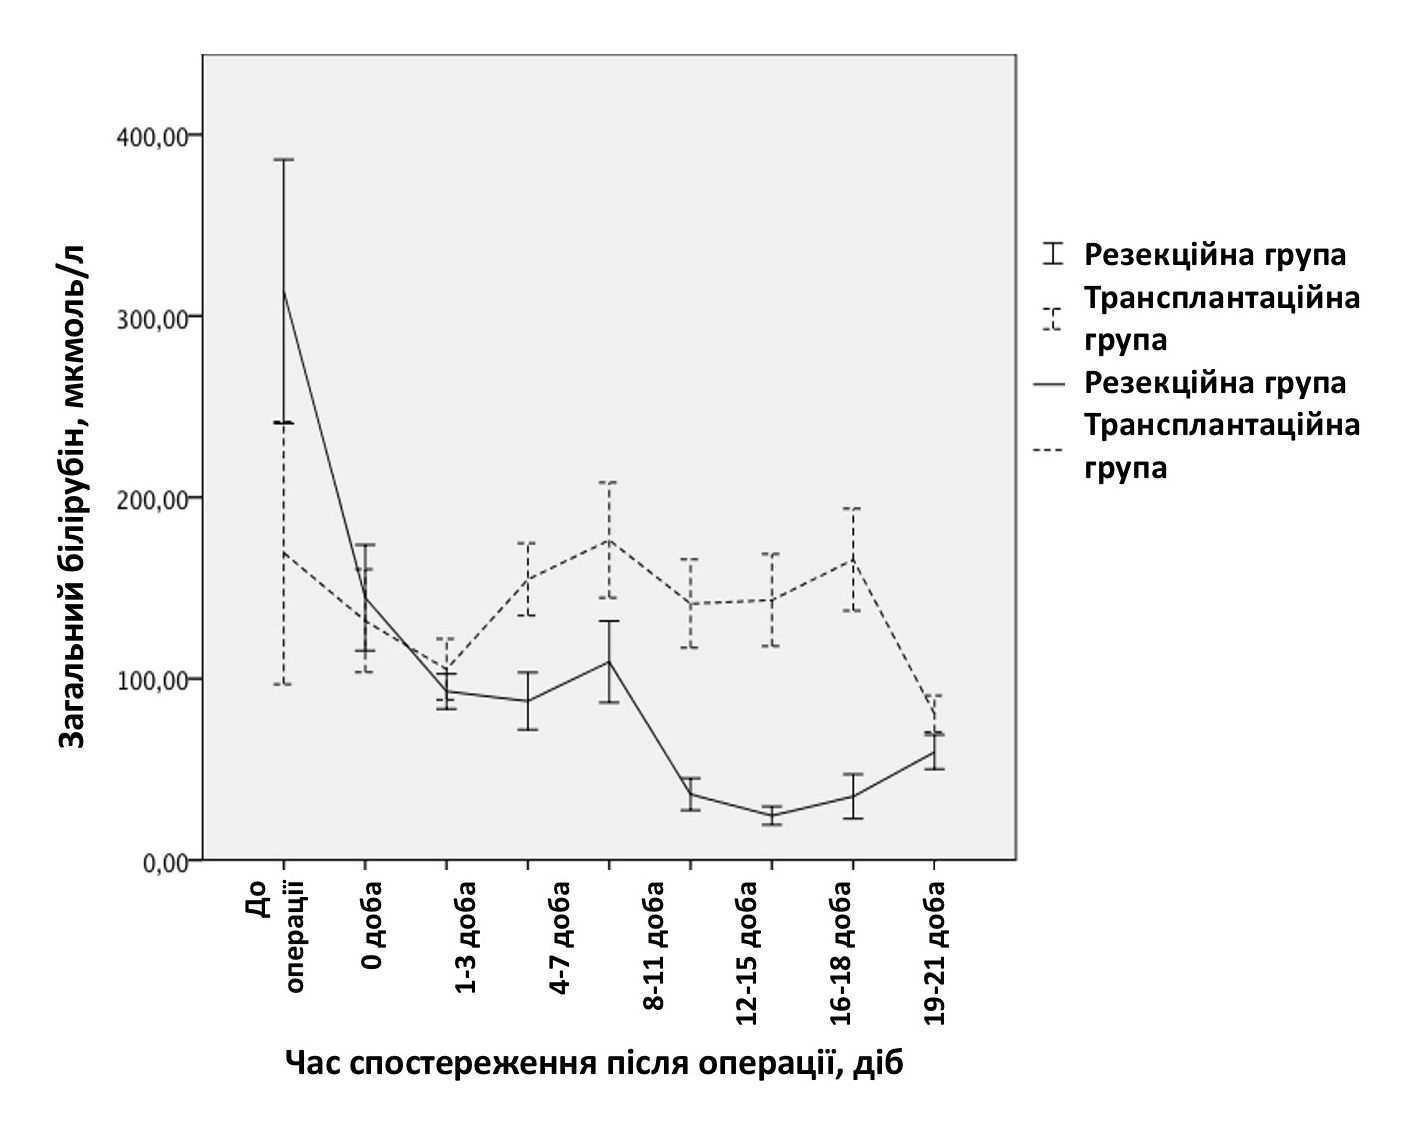
\includegraphics[width=0.7\textwidth]{Illustrations/graf/ZB.jpeg}
\label{fig:ZB} 
\end{figure}

Синтетичну функцію печінки оцінювали за рівнем показників коагулограми, загального білка та альбуміну сироватки крові (Рис. \ref{fig:alb})(Рис. \ref{fig:zbilok})(Рис. \ref{fig:pv}). Протромбіновий час у більшості реципієнтів внаслідок печінкової недостатності був значно підвищений у передопераційному періоді: 29,4±17,2 сек. у загальній вибірці, 31,2±21,0 сек. у трансплантаційній групі та 26±11,2 сек (Рис. \ref{fig:pv}). у резекцийній (відмінність між групами за методом Манна-Уітні статистично не значуща, р = 0,26). На 0-3 добу післяопераційного періоду значення протромбінового часу знижувалося до 257 ± 5 сек. у трансплантаційній групі та 23,5±4,8 у резекційній (р=0,18). Нормалізацію показника відзначали на 4-7 добу в обох групах. Надалі всі пацієнти отримували внутрішньовенну пролонговану інфузію гепарину з розрахунку 2-3 МО на кілограм маси тіла за хвилину для профілактики артеріальних тромбозів. Доза гепарину підбиралася для підтримки протромбінового часу на рівні 20-22 секунд. Після двох тижнів введення гепарину припиняли та призначали таблетовані антиагреганти (дипіридамол). Статистично значимих відмінностей між протромбіновим часом в групах виявлено не було. Значущість відмінностей між тимчасовими періодами була виявлена за допомогою критерію Фрідмана та підтверджена за допомогою тесту Вілкоксона на 1-3 (р=0,042) та 4-7(р=0,034) добу.

\begin{figure}[h]
\caption{Динаміка протромбіновго часу}
\centering
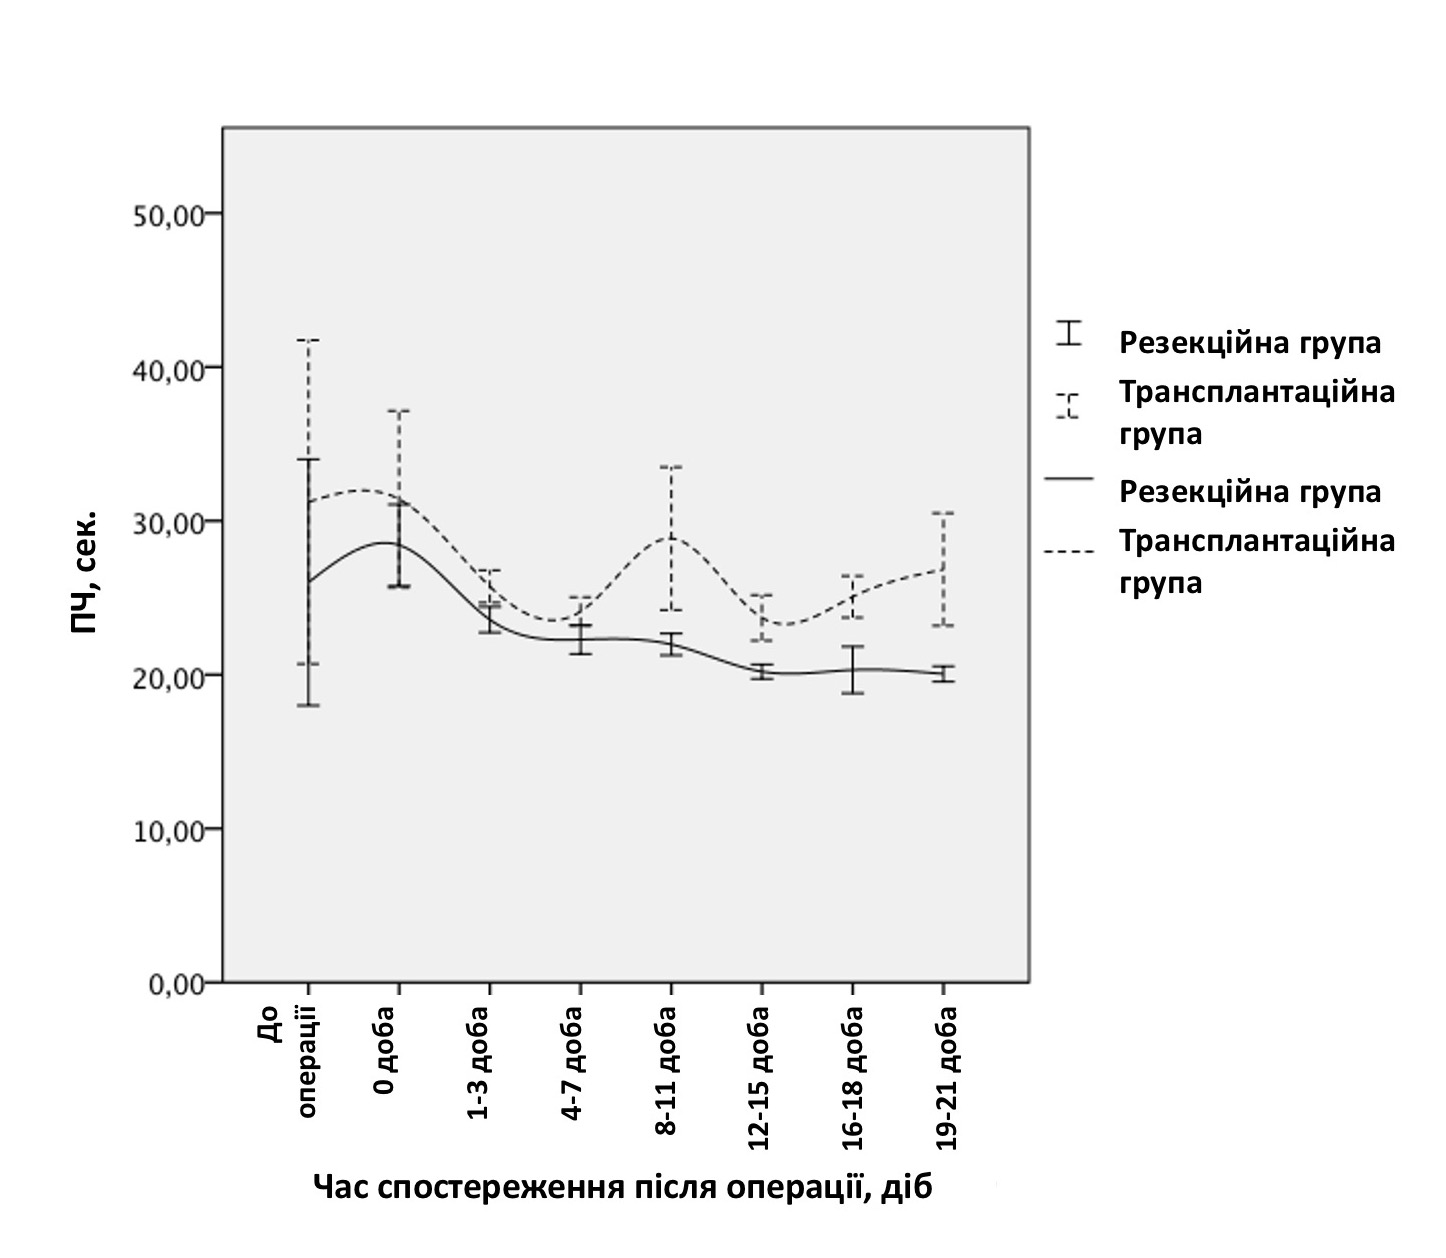
\includegraphics[width=0.7\textwidth]{Illustrations/graf/pv.jpeg}
\label{fig:pv} 
\end{figure}

Концентрація загального білка (Рис. \ref{fig:zbilok}) у сироватці крові реципієнтів резекційної групи та трансплантаційної групи до трансплантації склала 66,2±11,2 г/л та 60,7±6 г/л. На 0-3 добу після операції рівень загального білка в обох групах знижувався до 58,8±5,4 г/л у трансплантаційній та 64,1±5 г/л у резекційній групі. Нормалізація рівня загального білка відзначалася на 4-7 добу до 75±8,1 у трансплантаційній групі та на 12-15 добу до 82±9,2 резекційній. Значущість відмінностей між групами була виявлена тестом Крускала-Уолліса і підтверджена тестом Манна-Уітні до операції (р=0,03), на 0 добу (р=0,043), 1-3 добу (р=0,021), 4-7 добу ( р=0,03), 8-11 добу (р=0,05) та 12-15 добу (р=0,019). Значущість відмінностей між тимчасовими періодами була виявлена за допомогою критерію Фрідмана та підтверджена за допомогою тесту Вілкоксона на 0(р=0,032), 1-3(р=0,045), 4-7(р=0,05) та 12-15(р = 0,015) добу.

\begin{figure}[h]
\caption{Динаміка загального білка}
\centering
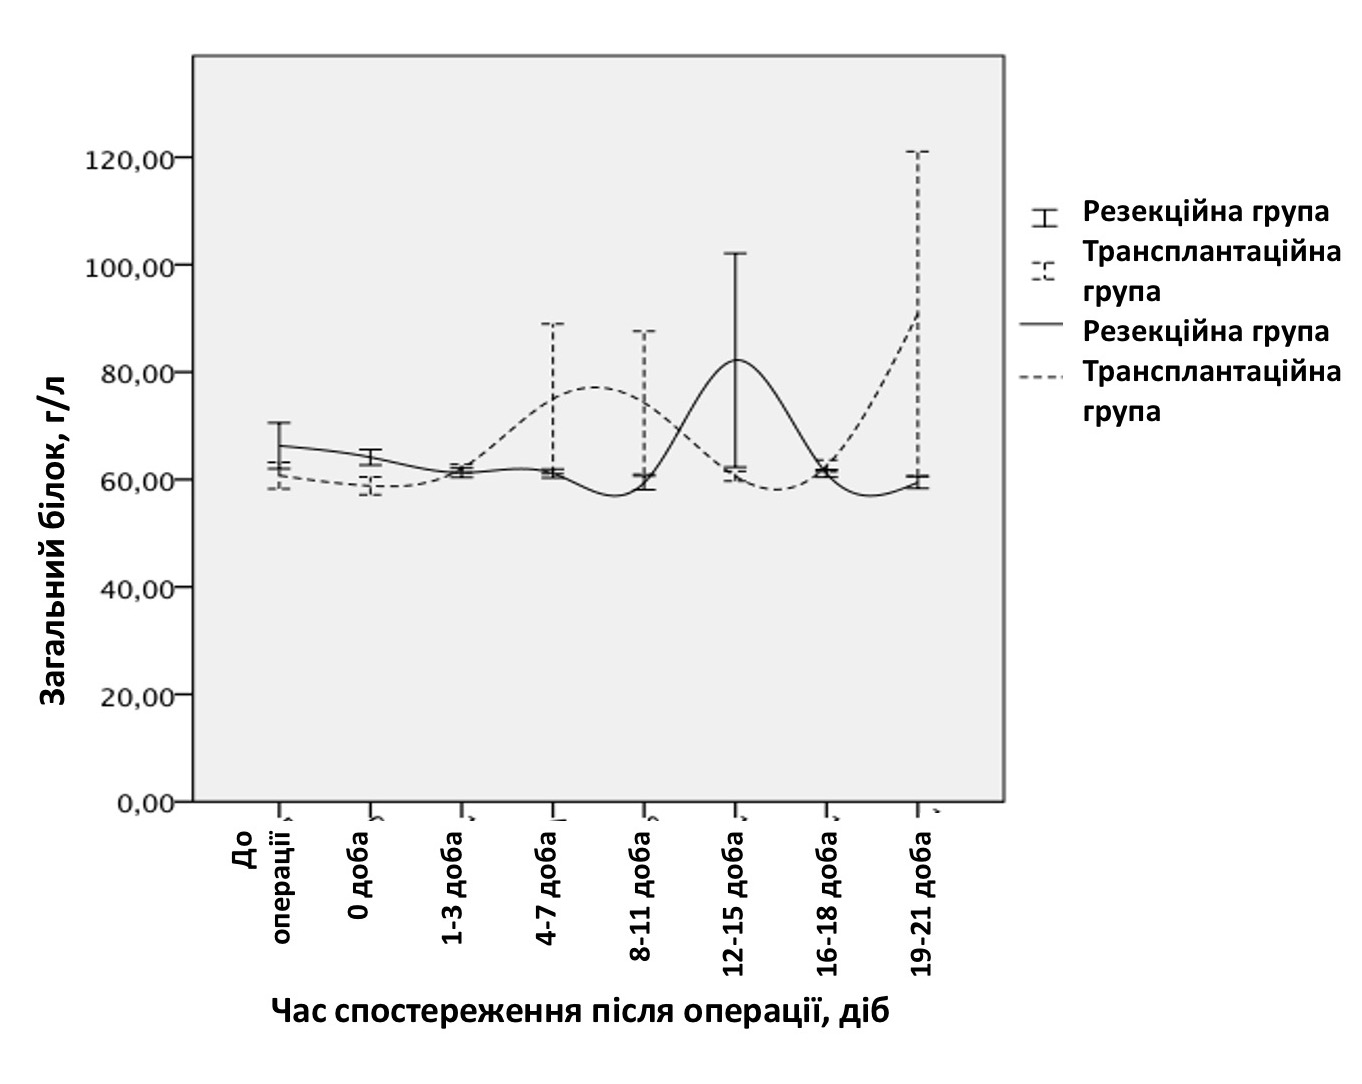
\includegraphics[width=0.7\textwidth]{Illustrations/graf/zbilok.jpeg}
\label{fig:zbilok} 
\end{figure}

Рівень концентрації альбуміну (Рис. \ref{fig:alb}) у сироватці крові обох груп реципієнтів до трансплантації був знижений і значуще між групами не відрізнявся – 32±1,4 г/л у трансплантаційній та 30±2,1 г/л у резекційній групі. У післяопераційному періоді на 0-3 добу в обох групах була відзначена нормалізація рівня білірубіну до 36,6±6 г/л в трансплантаційній та 36,7±5 г/л в резекційній групі внаслідок масивного замісного інтраопераційного переливання альбуміну. Починаючи з 4 доби післяопераційного періоду, рівень альбуміну знижувався в обох групах, але більш значне зниження відзначали резекційній. Різниця між рівнями альбуміну в групах була найбільш виражена на 8-11 добу – 32,8±6 г/л у трансплантаційній та 29,6±3 г/л у резекційній групі.

\begin{figure}[h]
\caption{Динаміка загального альбуміну}
\centering
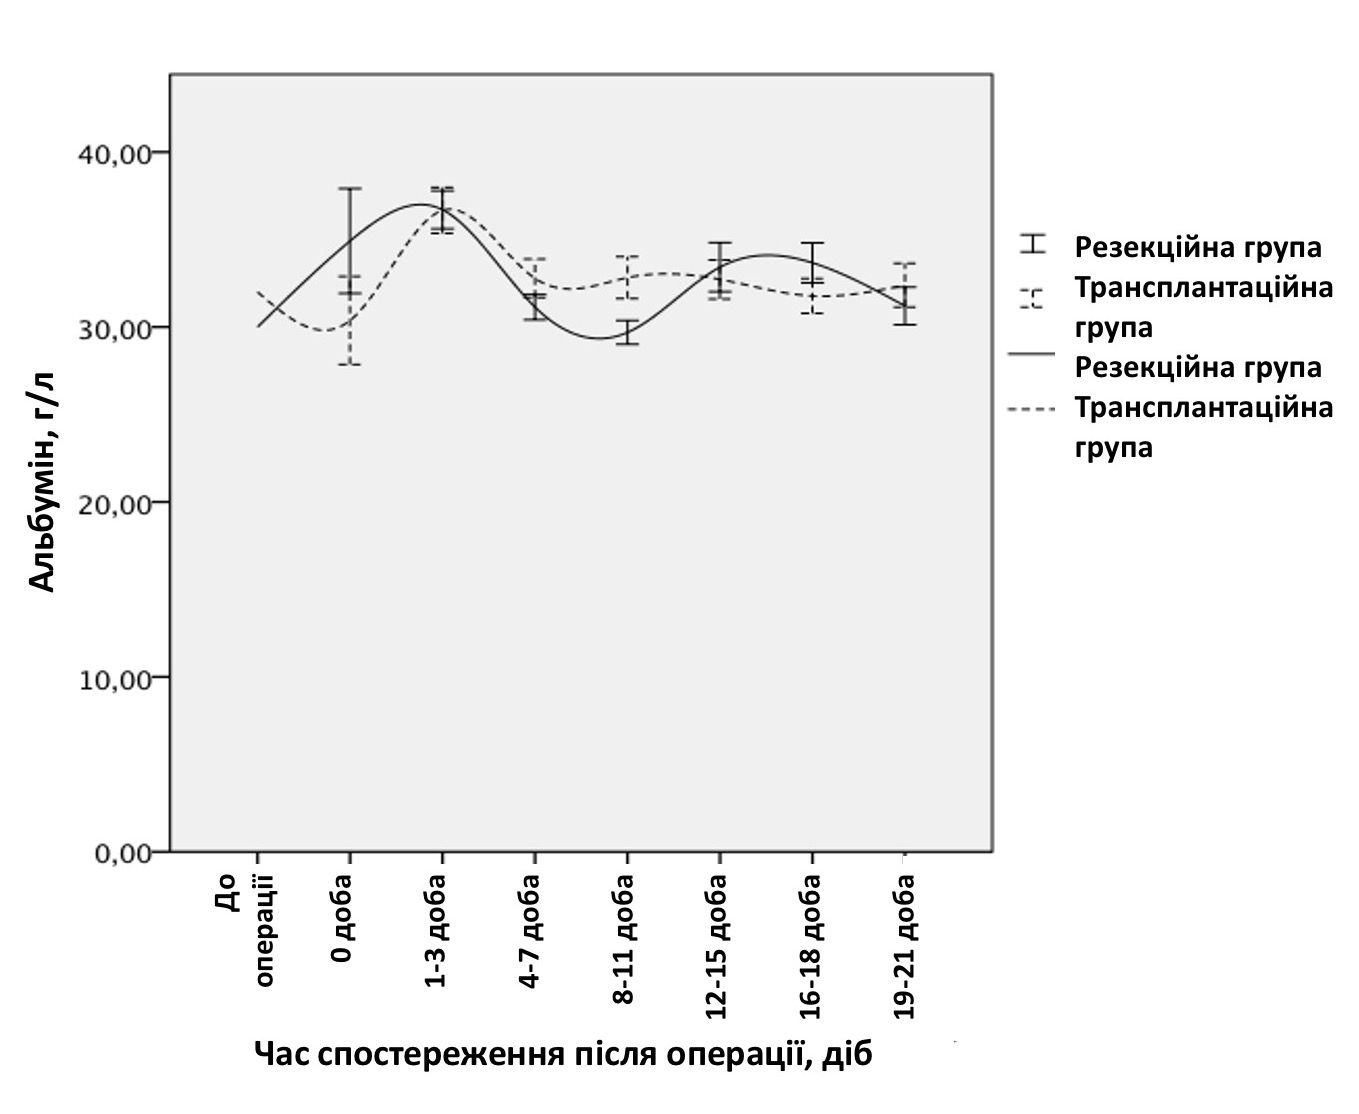
\includegraphics[width=0.7\textwidth]{Illustrations/graf/alb.jpeg}
\label{fig:alb} 
\end{figure}

Починаючи з 12 доби в обох групах відзначали нормалізацію рівня альбуміну – до 33,2±7 г/л у трансплантаційній та 33,4±3 г/л у резекційній групі. Статистична значущість відмінностей між групами була виявлена тестом Крускала-Уолліса та підтверджена тестом Манна-Уітні на 4-7 добу (р=0,021) та 8-11 добу (р=0,01). Значущість відмінностей між тимчасовими періодами була виявлена за допомогою критерію Фрідмана та підтверджена за допомогою тесту Вілкоксона на 0(р=0,024), 1-3(р=0,05), 4-7(р=0,01) та 8-11 (Р = 0,03) добу. Така різниця в динаміці концентрації загального білка та альбуміну сироватки крові обумовлена більшою частотою печінкової недостатності та асцитопродукції у резекційній групі порівняно з трансплантаційною.

Наявність дисциркуляторних змін у паренхімі трансплантату опосередковано оцінювали за рівнем цитолітичних ферментів – аланінамінотрансферази (АЛТ) та аспартатамінотрансферази (АСТ). Рівень АЛТ (Рис. \ref{fig:alt}) в обох групах до операції не відрізнявся, і складав 107±83 ОД у трансплантаційній та 106±97 ОД резекційній групі. У післяопераційному періоді рівень АЛТ зростав в обох групах. Максимальне підвищення активності АЛТ у трансплантаційній групі припадало на 4-7 добу і становило 328±71 ОД, а в резекційній групі на 1-3 добу та становило 272±38 ОД. Нормалізацію активності АЛТ відзначали на 16-18 добу в обох групах. Статистично значущої відмінності між групами не виявлено. Значущість відмінностей між тимчасовими періодами була виявлена за допомогою критерію Фрідмана та підтверджена за допомогою тесту Вілкоксона на 0(р=0,004), 1-3(р=0,041), 4-7(р=0,011) та 8-11(р=0,023) добу.

\begin{figure}[h]
\caption{Динаміка АЛТ}
\centering
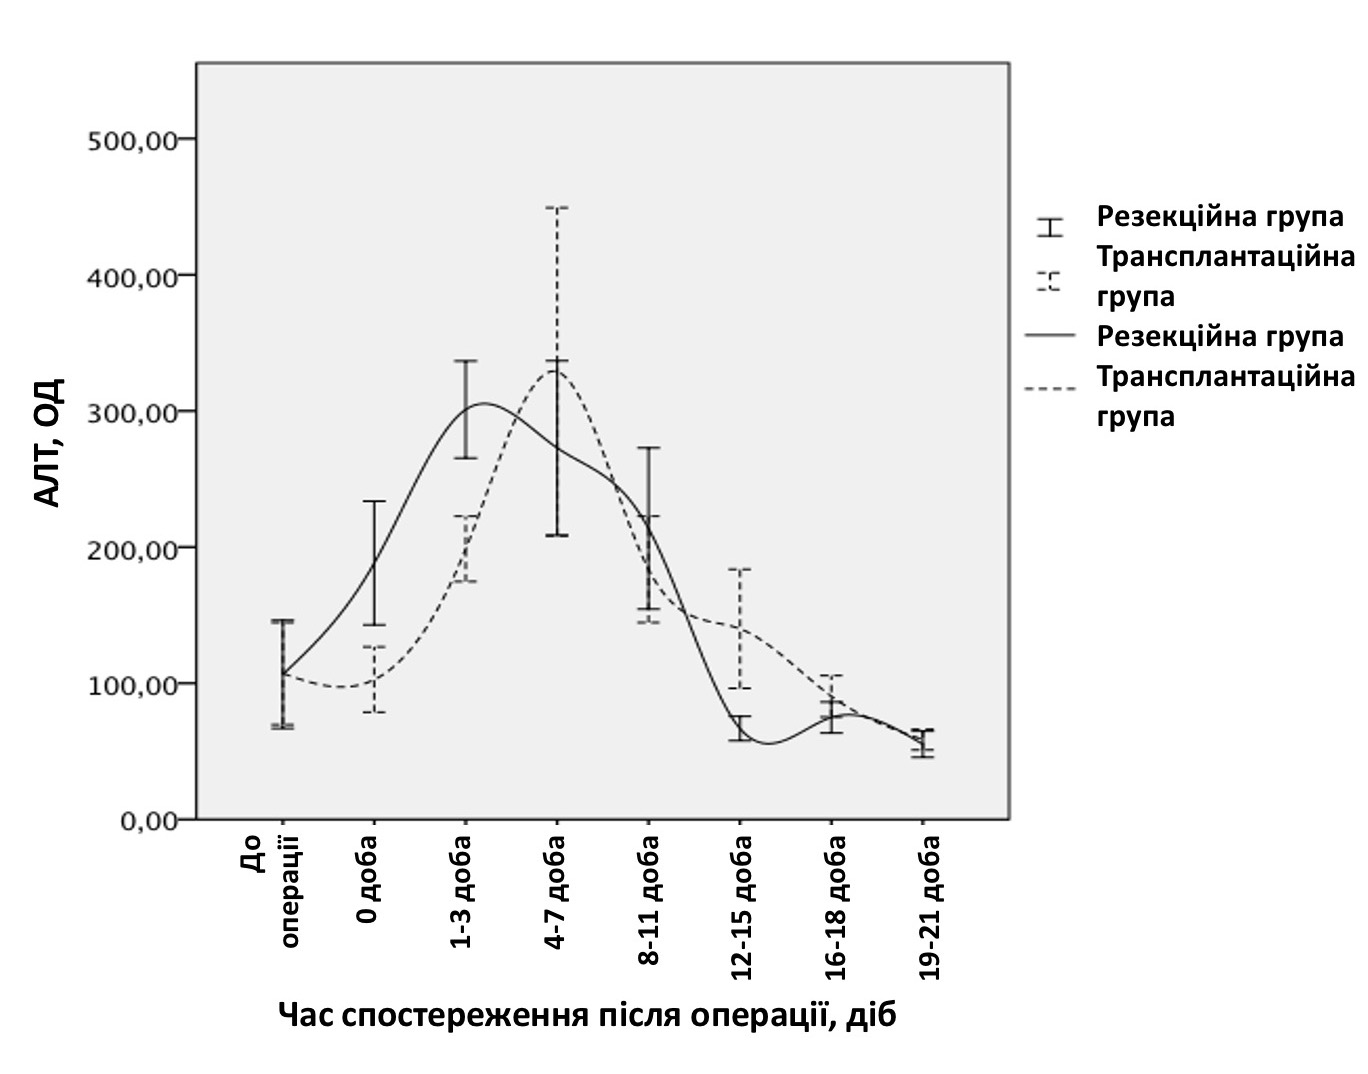
\includegraphics[width=0.7\textwidth]{Illustrations/graf/alt.jpeg}
\label{fig:alt} 
\end{figure}

Рівень АСТ (Рис. \ref{fig:ast}) також у доопераційному періоді у групах статистично значимо не відрізнявся і становив 179±15 ОД у трансплантаційній групі та 177±21 ОД резекційній. У післяопераційному періоді відзначалося підвищення рівня активності АСТ в обох групах. Максимальне підвищення активності АСТ у трансплантаційній групі припадало на 4-7 добу і становило 323 ± 77 ОД, а в резекційній на 1-3 добу і становило 270 ± 18 ОД.

\begin{figure}[h]
\caption{Динаміка АСТ}
\centering
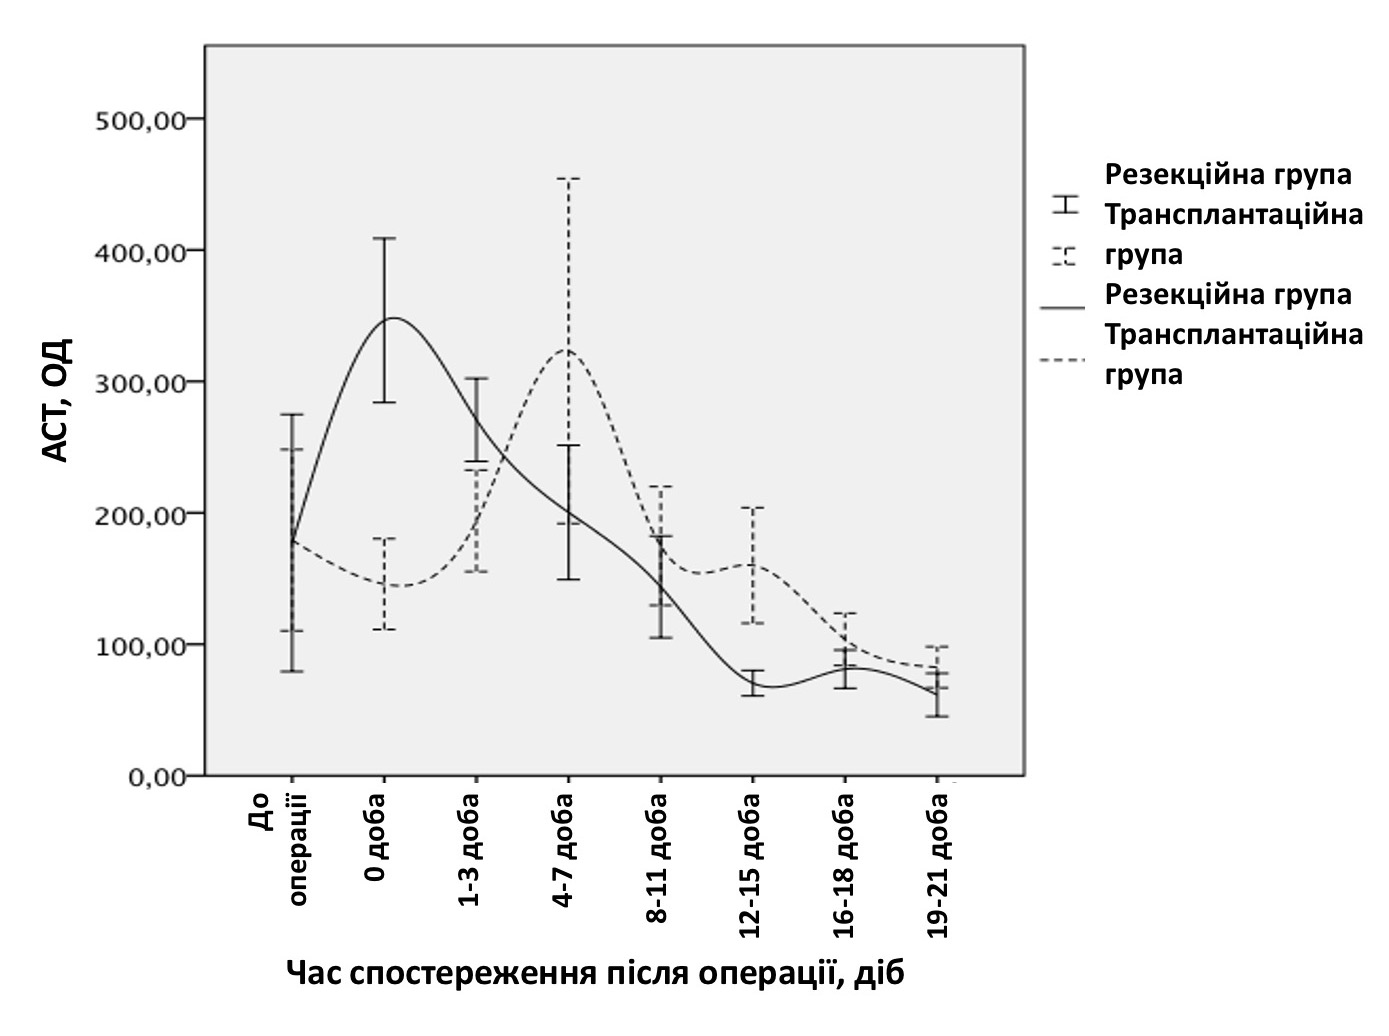
\includegraphics[width=0.7\textwidth]{Illustrations/graf/ast.jpeg}
\label{fig:ast} 
\end{figure}

Нормалізацію активності АЛТ відзначали на 16-18 добу в обох групах. Статистичної значущості відмінностей між групами не виявлено. Значимість відмінностей між тимчасовими періодами була виявлена за допомогою критерію Фрідмана та підтверджена за допомогою тесту Вілкоксона на 0(р=0,03), 1-3(р=0,023), 4-7(р=0,021), 8-11 (p =0,019) та 16-18(р=0,031) добу.
Підвищення активності цитолітичних ферментів у педіатричних реципієнтів пов'язане з наявністю ішемічного ушкодження під час відмивання трансплантату та перфузійного ушкодження при розвитку гіпердинамічного портального кровотоку в ранньому післяопераційному періоді, що підтверджує їх нормалізація на другому тижні післяопераційного періоду.




\section{Порівняльна оцінка віддалених післяопераційних результатів}

Рання післяопераційна летальність в стаціонарі (до 30 діб) в резекційній групі склала 4 (4,9\%) пацієнтів, і не було леталності в трансплантаційній групі. 
Для розрахунку загальної та безрецидивної виживаності по групах використали метод Каплан-Мейєра, значимість відмінностей в групах визначали з допомогою критерія Log-rank и Breslow. криві виживаності представлені на (Рис. \ref{fig:os1}) та (Рис. \ref{fig:dfs1}). Форма кривих свідчить про те, що найбільш критичним печіодом для пацієнтів ж перші 3 місяці післяопераційного періоду. В подальшому післяопераційному періоді ризик летального випадку значно зменшується. 
Для оцінки віддалених результатів хірургічного лікування гепатобластоми з допомогою резекції печінки та трансплантації досліджували виживання протягом 1, 2-х і 3-х років після операції. Загальна 1, 3, 5 річна виживаність у резекційній групі склала 92,3\%, 82,7\%, 71,1\% відповідно. У трансплантаційній групі 1, 3, 5 річна виживаність склала 100\%, 87,5\%, 75\% відповідно (Рис. \ref{fig:os1}).

\begin{figure}[h]
\caption{Загальна виживаність пацієнтів з гепатобластомою.}
\centering
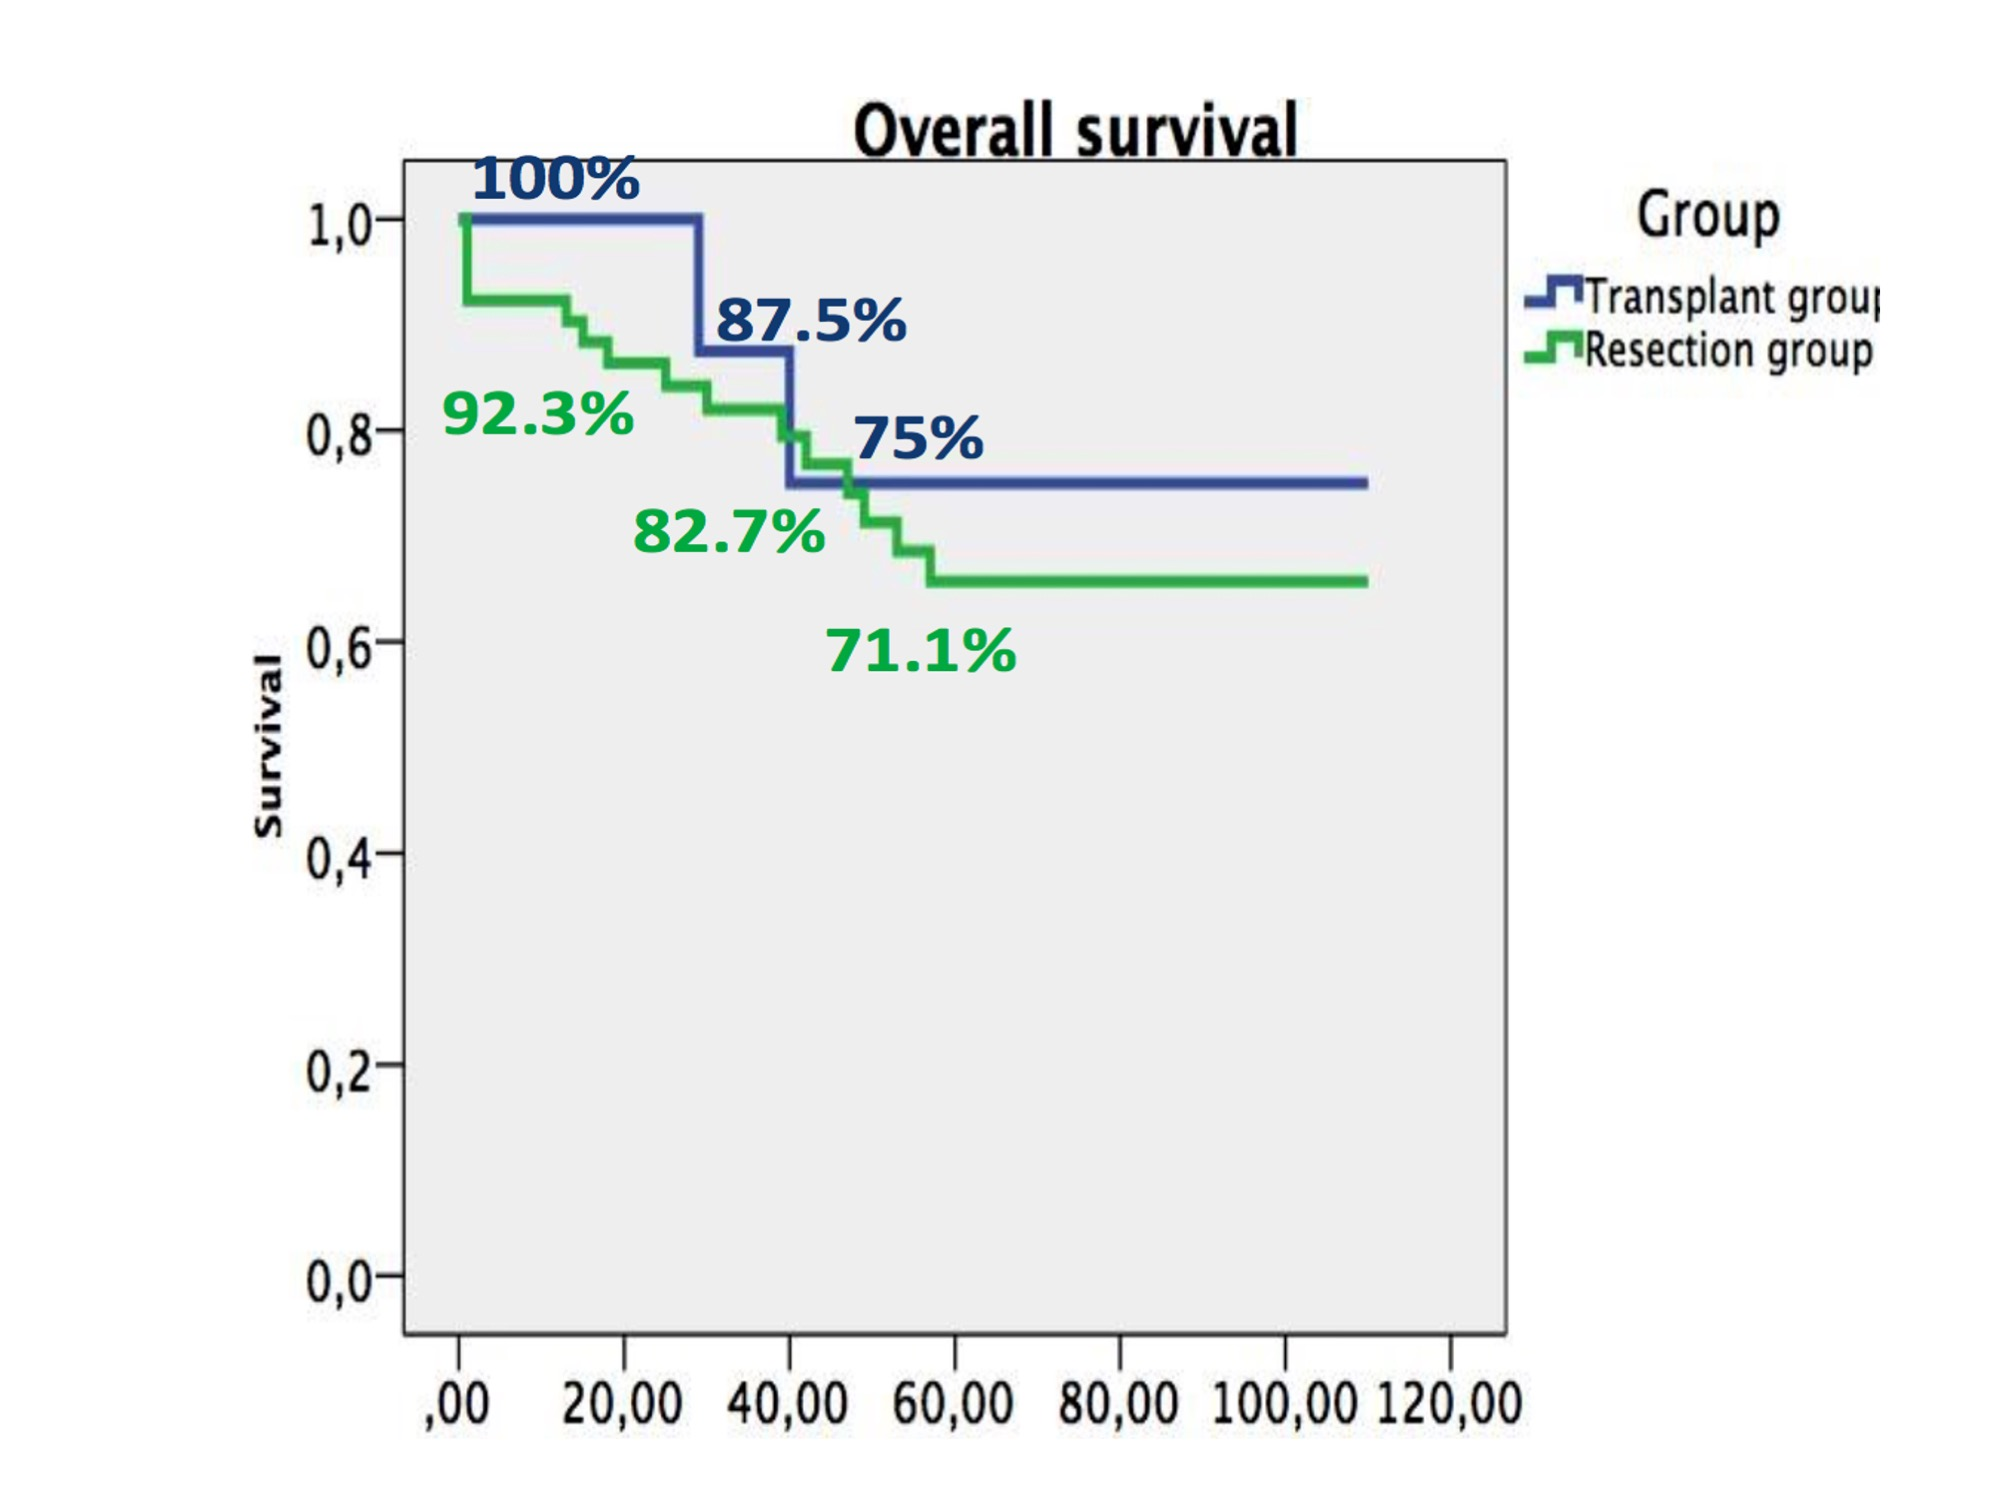
\includegraphics[width=0.8\textwidth]{Illustrations/os1.jpg}
\label{fig:os1} 
\end{figure}


Безрецидивна 1, 3, 5 річна виживаність у резекційній групі склала 86,5\%, 76,6\%, 69,2\% відповідно. У трансплантаційній групі 1, 3, 5 річна виживаність склала 87,5\%, 75,0\%, 62,5\% відповідно (Рис. \ref{fig:dfs1}).

\begin{figure}[h]
\caption{Безрецидивана виживаність пацієнтів з гепатобластомою.}
\centering
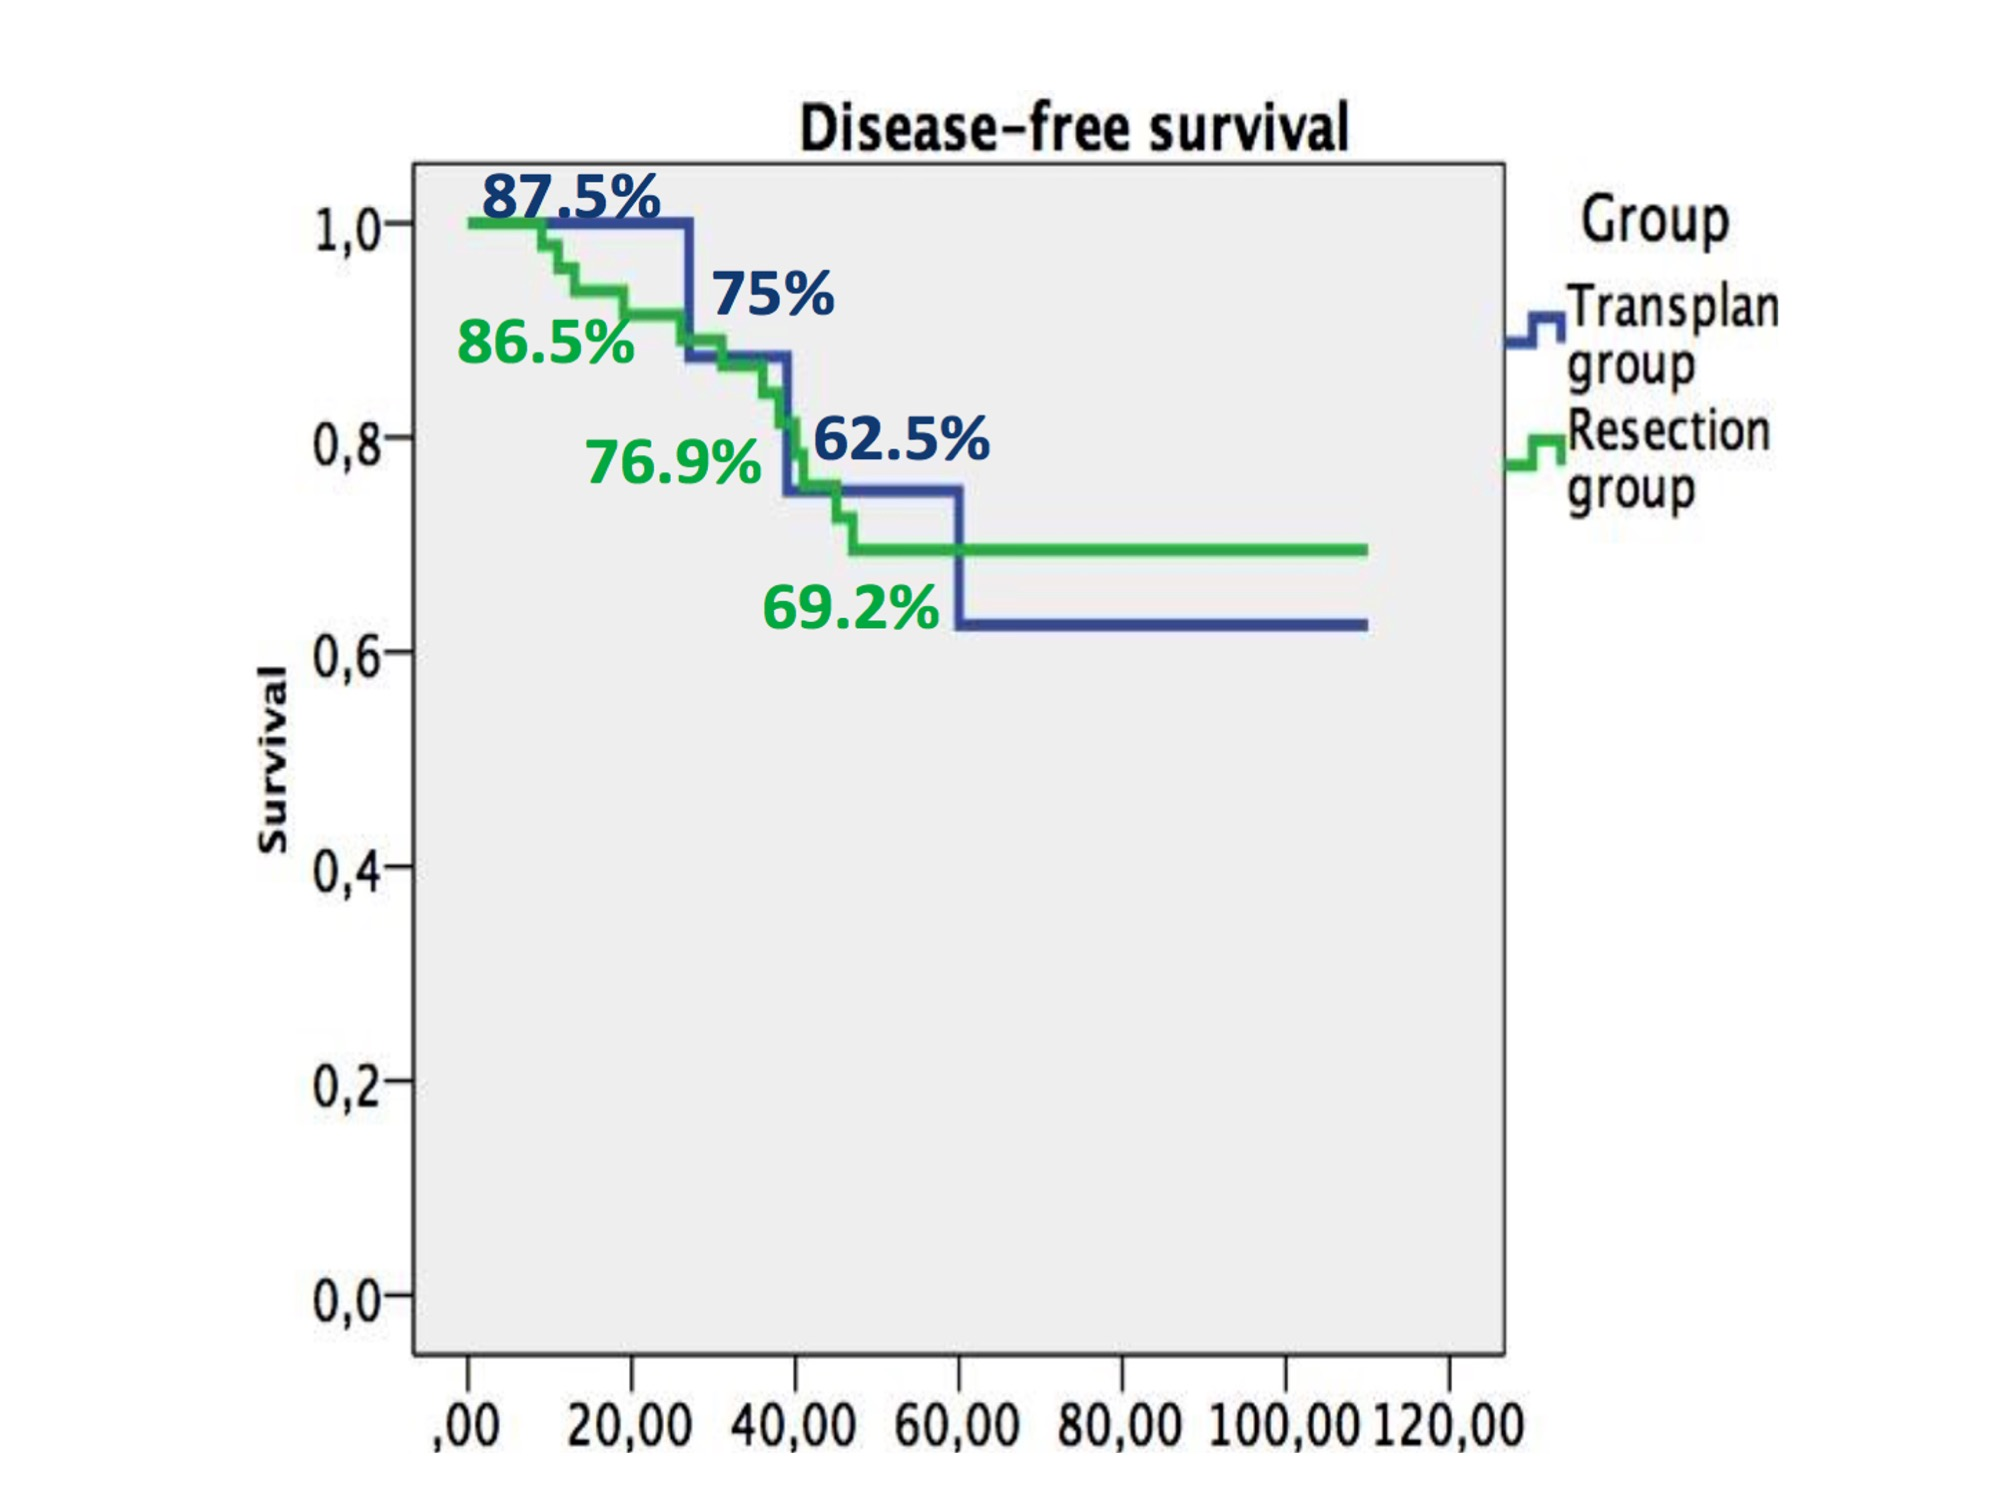
\includegraphics[width=0.8\textwidth]{Illustrations/dfs1.jpg}
\label{fig:dfs1} 
\end{figure}

\section{Алгоритм вибору тактики лікування у пацієнтів з гепатобластомою}
Базуючись на використанні запропонованої нами тактики лікування пацієнтів з гепатобластомою, нами було розроблено алгоритм вибору тактики лiкування у пацiєнтiв з гепатобластомою. Алгоритм базується на результатах доопераційної діагностики та стадіювання пацієнтів Рис. \ref{fig:algoritmmm}).

При визначенні тактики лікування беремо до уваги стадію гепатбластоми по PRETEX, а також її субкласифікації (наявність віддалених метастазів, інвазії в ворітну вену, печінкові або нижню порожнисту вени). 
Після чого визначаємо групу ризику пацієнта по системі CHICS (Children’s Hepatic Tumors International Collaboration`s Stratification), де беремо до уваги такі показники як вік, рівень АФП, інвазію судин та наявність метастазів пухлини та розприділяємо пацієнтів на групи ризику: LR – група низького ризику, IR – група середнього ризику, HR – група високого ризику та VHR – група вкрай високого ризику (Рис. \ref{tab:risk}).

Наступним етапом діагностики є біопсія пухлини. 
В залежності від групи ризику призначається неоадювантна хіміотерапія. 

Після отримання неоадювантної хіміотерапії та нормальлізації гематологічних показників крові, виконується оперативне втручання. Об'єм оперативного втручання залежить від стадії гепатобластоми. За звичай при пухлинах PRETEX І-ІІІ виконували резекції печінки, при PRETEX IV - трансплантацію печінки (Рис. \ref{fig:algoritmmm}).

При наявності резектабельного метастазу, після неоадювантної хіміотерапії при стабілізації пухлини та метастазу проводили метастазектомію. Після оперативного лікування (резекції, тарнсплантації, метастазектомії) після нормалізації стану пацієнта проводили адювантну хіміотерапіз згідно плану (Рис. \ref{fig:algoritmmm}).

В післяопераційному періоді проводимо спостереження у у випадку появи рецидиву або метастазування проводимо повторну резекцію печінки або метастазектомію. 

\begin{figure}[h]
\caption{Алгоритм діагностики і лікування гепатобластоми в залежності від групи ризику}
\centering
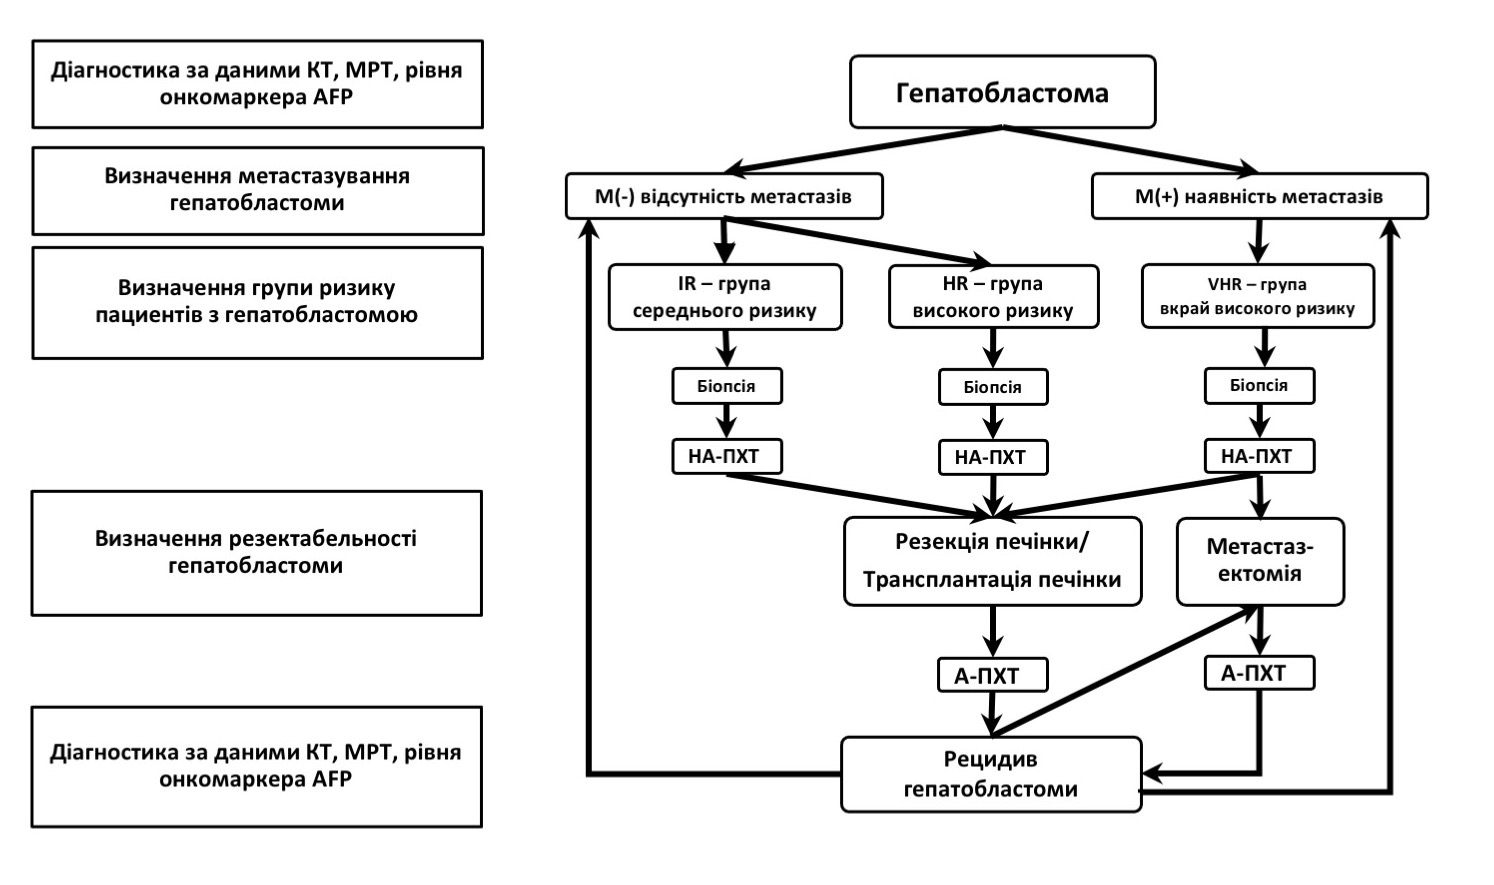
\includegraphics[width=0.9\textwidth]{Illustrations/algoritmmm.jpg}
\label{fig:algoritmmm} 
\end{figure}

%\chapter{Малюнки та таблиці}

\section{Перелік необхідних таблиць}

\begin{enumerate}
    
    \item Первинна локалізація ураження у пацієнтів з ГБ (по сегментах, PRETEXT, частота для загальної групи пацієнтів) 
    \item Патоморфологічні варіанти ГБ 
    \item Режими та Ефективність пхт (частота конверсії в резектабельні форми, частота редукції позаорганних проявів) 
    \item Розподіл антропометричних показників (вік, вага, зріст) та коморбідності в загальній виборці та по группах.  ???
    \item Характеристика ураження печінки в загальній виборці та по группах 
    \item Характеристика донорів в трансплантаційній групі (антропометричні показиники, коморбідність) 
    \item Критерії підбору донорів -----
    \item Характеристика оперативних втручань та судинних резекцій в резекційній групі 
    \item Характеристика оперативних втручань в трансплантаційній групі 
    \item Порівняльна характеристика ранніх післяопераційних ускладненнь та летальності 
    \item Причини післяопераційної летальності
    \item Порівняльна характеристика післяопераційної печінкової недостатності. ??????
    \item Порівняльна характеристика віддалених результатів лікування ГБ 
    
\end{enumerate}

\section{Перелік необхідних малюнків}

\begin{enumerate}
    \item PRETEXT (з інтернету, замінити підписи) 
    \item CHICS (з інтернету, замінити підписи) 
    \item Алгоритм діагностики гепатобластоми
    \item Дизайн дослідження (2 групи - трансплантація та резекція на основі результатів ПХТ - схема в поверпоінті
    \item Критерії резектабельності гепатобластоми (та покази до трансплантації)
    \item Критерії операбельності гепатобластоми 
    \item Способи реконструкції портального притоку при трансплантації печінки з приводу ГБ
    \item Способи реконструкції венозного відтоку при трансплантації печінки з приводу ГБ
    \item Алгоритм вибору хірургічного способу лікування ГБ
    
    
\end{enumerate}

%\chapter{ПРИКЛАД НАЗВИ РОЗДІЛУ, ЯКИЙ ПИШЕТЬСЯ ВЕЛИКИМИ ЛІТЕРАМИ. СЛОВО "РОЗДІЛ" ТА НОМЕР ПИСАТИ НЕ ПОТРІБНО}


\section{Назва секції, буде відображена у змісті звіту}

Звичайний параграф тексту, що містить тільки текст. Звичайний параграф тексту, що містить тільки текст. Звичайний параграф тексту, що містить тільки текст. Звичайний параграф тексту, що містить тільки текст. Звичайний параграф тексту, що містить тільки текст.

Звичайний параграф тексту, що містить текст та посилання. Звичайний параграф тексту, що містить текст та посилання. Звичайний параграф тексту, що містить текст та посилання. Текст після якого йде посилання \cite{Chen2019}. 


\section{Інша назва секції}
\subsection{Інша назва субсекції}

\noindent Звичайний параграф тексту, без відступу червоної строки. Звичайний параграф тексту, без відступу червоної строки. Звичайний параграф тексту, без відступу червоної строки. Звичайний параграф тексту, без відступу червоної строки. Звичайний параграф тексту, без відступу червоної строки. % \noindent - знімає відступ в параграфі тексту

Строка із символом переносу каретки \\ % символ "\\"  це кінець строки або перенос каретки

\noindent \textbf{Жирний текст} \\
\noindent \textit{Курсивний текст} \\

\section{Вставка іллюстрацій}

Звичайний параграф тексту, в якому міститься згадування про малюнок. Звичайний параграф тексту, в якому міститься згадування про малюнок. Звичайний параграф тексту, в якому міститься згадування про малюнок. Звичайний параграф тексту, в якому міститься згадування про малюнок. (Рис. \ref{fig:NameOfPicture}) % Назва малюнку (нумерація відбувається автоматично)
Звичайний параграф тексту, в якому міститься згадування про малюнок. Звичайний параграф тексту, в якому міститься згадування про малюнок. 


% блок вставки малюнка
\begin{figure}[h]
\caption{Заголовок малюнку із посиланням \cite{Chen2019}}
\centering

\includegraphics[width=0.9\textwidth]{Illustrations/Logo.png}
\label{fig:NameOfPicture} % Назва малюнку
\end{figure}
% кінець блоку вставки малюнка

Звичайний параграф тексту, в якому міститься згадування про малюнок. (Таб. \ref{table:NameOfTable}) % Назва малюнку (нумерація відбувається автоматично)
Звичайний параграф тексту, в якому міститься згадування про малюнок. Звичайний параграф тексту, в якому міститься згадування про малюнок. 
% Please add the following required packages to your document preamble:
% \usepackage{graphicx}



\section{Нумеровані та ненумаровані списки}

Це нумерований список

\begin{enumerate}
    \item Позиція 
    \item Інша позиція
    \item Ще одна позиція
\end{enumerate}

\vspace{2em} % це відступ

Це ненумерований список

\begin{itemize}
    \item Позиція 
    \item Інша позиція
    \item Ще одна позиція
\end{itemize}
    
\backmatter
%%%%%%%%%%%%%%%%%%%%%%%%%%%%
%%%%%%%%%%%%%%%%%%%%%%%%%%%%

\chapter{АНАЛІЗ ТА УЗАГАЛЬНЕННЯ РЕЗУЛЬТАТІВ ДОСЛІДЖЕННЯ}

\textbf{Тут повинні бути висновки, які є в кінці кожного розділу:}

ТЕКСТ ПРИБЛИЗНИЙ - тут тільки основна ідея!!!

Проведений аналіз літературних джерел дозволив встановити, що є велика кількість нерезектабельних пацієнтів яким можливо виконати трансплантацію

Загальна частота виникнення гепатобластоми скаладає .... 

Ефективність неоадьювантної поліхіміотерапії ....

Резектабельнісь визначається ....

Для виконання поставлених задач нами було досліджено .....

Тактика лікування гепатобластоми включає ....

Особливістю резекційного методу є необхідність судинних реконструкцій у випадках судинних інвазій .....

Особливостями трансплантаційного методу є .....

Запропонований алгоритм із залученням запропонованих способів дозволяє отримати ......


\chapter{ВИСНОВКИ}
\begin{enumerate}
    \item При первинній діагностиці в \% випадків спостерігали неоперабельні форми гепатобластоми. Проведення поліхіміотерапії за схемою PLADO дозволило отримати конверсію в операбельні форми у \% з цих пацієнтів, та підвищити загльний рівень операбельності до  \%.
    
    \item З усіх відомих гістологічних форм частіше (у \% випадків) зустрічали ...... та .... форми гепатобластоми. Наявність у пацієнта ..... форми була визначена в \% випадків та пов'язана із погіршенням прогнозу та зменшенням післяопераційної виживаності до \%.
    
    \item Вибір резекційного або трансплантаційного методу хірургічного лікування визначається резектабельністю пухлини, яка залежить від ступеня її поширеності за PRETEXT та наявності інвазії в магістральні судини. У \% пацієнтів з резектабельними формами гепатобластоми були виконані обширні резекції печінки, а у \% з нерезектабельними - трансплантація частини печінки від живого родинного донора із використанням розроблених способів венозної реконструкції.
    
    \item Резекційний метод хірургічного лікування гепатобластоми включав виконання розширених (у \% пацієнтів) та обширних (у \% пацієнтів) резекцій печінки із пластикою нижньої порожнистої вени в \% та портопластикою в \%.
    
    \item Транслантаційний метод хірургічного лікування гепатобластоми включав трансплантацію лівої латеральної секції печінки (у \% пацієнтів) та лівої долі печінки (у \% пацієнтів) від живого родинного донора із використанням запропонованих способів венозної реконструкції в \%.
    
    \item Впровадження запропонованої тактики вибору резекційного або трансплантаційного методу хірургічного лікування дозволило збільшити кількість операбельних форм гепатобластоми на  \% за рахунок виконання трансплантації печінки нерезектабельним пацієнтам, та отримати задовільні показники післяопераційної морбідності, летальності та віддаленої виживансоті на рівні   \% \% та \% відповідно.
    
\end{enumerate}

%%%%%%%%%%%%%%%%%%%%%%%%%
%       Бібліографія    %
%%%%%%%%%%%%%%%%%%%%%%%%%
\clearpage
\addcontentsline{toc}{chapter}{ПЕРЕЛІК ПОСИЛАНЬ}
%\bibliographystyle{gost780}
% \bibliographystyle{unsrt}
 \bibliographystyle{plain}
\bibliography{Bibliography/literature}
%%%%%%%%%%%%%%%%%%%%%%%%%%%%
%%%%%%%%%%%%%%%%%%%%%%%%%%%%



%%%%%%%%%%%%%%%%%%%%%%%%%
%       Додатки         %
%%%%%%%%%%%%%%%%%%%%%%%%%

\appendix
\updatechaptername

\chapter{Практичні рекомендації}
\newpage
~
\newpage
~


%%%%%%%%%%%%%%%%%%%%%%%%%%%%
%%%%%%%%%%%%%%%%%%%%%%%%%%%%


\end{document}
